This chapter provides the necessary background on solar radiation in the Martian environment. \refSec{sec:MarsSolarEnergy:SolarRadiation} introduce variables and equations that must will be used when analyzing solar irradiance and insolation on Mars. Power and energy equations are presented in \refSec{sec:MarsSolarEnergy:PhotovoltaicEnergy}. \refSec{sec:MarsSolarEnergy:MissionSites} reviews the selected mission sites and presents their worst case daily insolations. The chapter is summarized and concluded in \refSec{sec:MarsSolarEnergy:SummaryAndConclusion}.

\section{Solar Radiation}
\label{sec:MarsSolarEnergy:SolarRadiation}
%\input{sections/mars-solar-energy/solar-radiation/references.tex}
\todo[inline]{\textbf{TODO:} Write section introduction.}

\subsection{Seasons}
\label{sec:MartianEnvironment:Seasons}
The red planet's axis is tilted away from the sun at \SI{25}{\degree}. Very much like Earth's \SI{23.5}{\degree} axial tilt, this results in seasons. Mars has an orbit with a semi-major axis of \SI{1.524}{\astronomicalunit} which translates to a Martian year corresponding to an orbital period of 687 days. Martian seasons are longer and for every Martian year 1.88 Earth years go by. Sidereal days are 24.62 hours long and solar days are 24.65 hours long. A Martian day, known as a Sol, is approximately 40 minutes longer than an Earth day. Mars' position on its orbit is described in terms of areocentric longitude of the Sun, $L_{s}$, and is measured Eastwards from $L_{s} = \SI{0}{\degree}$ at the northern hemisphere's Vernal equinox. The transition of Martian seasons are presented in Table \ref{tab:mars-seasonal-advances} with respect to areocentric longitudes.

\begin{table}[H]
  \footnotesize
  \centering
  \caption{Seasonal advances on Mars.}
  \label{tab:mars-seasonal-advances}
  \begin{tabular}{|l|l|l|}
  \hline
  \multirow{2}{*}{\textbf{\begin{tabular}[c]{@{}l@{}}Areocentric\\ Longitude\end{tabular}}} & \multicolumn{2}{c|}{\textbf{Seasonal Advance}} \\ \cline{2-3}
   & \multicolumn{1}{c|}{\textbf{Northern Hemisphere}} & \multicolumn{1}{c|}{\textbf{Southern Hemisphere}} \\ \hline
  \si{0}{\degree} & Vernal Equinox & Autumnal Equinox \\ \hline
  \si{0}{\degree} to \si{90}{\degree} & Spring & Autumn \\ \hline
  \si{90}{\degree} & Summer Solstice & Winter Solstice \\ \hline
  \si{90}{\degree} to \si{180}{\degree} & Summer & Winter \\ \hline
  \si{180}{\degree} & Autumnal Equinox & Vernal Equinox \\ \hline
  \si{180}{\degree} to \si{270}{\degree} & Autumn & Spring \\ \hline
  \si{270}{\degree} & Winter Solstice & Summer Solstice \\ \hline
  \si{270}{\degree} to \si{360}{\degree} & Winter & Summer \\ \hline
  \end{tabular}
\end{table}


\clearpage
\subsection{Dust}
\label{sec:MartianEnvironment:Dust}
The Martian surface is aeolianly active with varying concentration of airborn dust throughout the year due to processes of dust lifting, transportation, and deposition \citemarsenv{Kahre2006}.

\todo[inline]{\textbf{TODO:} Short overview of dust cycle on Mars.}
% See: https://www.nasa.gov/feature/goddard/2018/curiosity-photos-show-martian-dust-storm-growing

\subsubsection{Atmospheric Opacity}
\label{sec:MartianEnvironment:Dust:AtmosphericOpacity}
The density of suspended dust determines the atmospheric opacity, or optical depth, measured in $\tau$ factors. A $\tau$ factor between 0 and 0.5 indicates a clear to relatively clear day. Higher $\tau$ factors indicate dusty days with growing atmospheric dust opacity as represented in Figure \ref{fig:image:tau-factors} for simulated views pointing towards the Sun. \SI{99}{\percent} of sunlight is blocked at $\tau$ factor 4.7.

\todo[inline]{\textbf{TODO:} Source the 99\% claim.}

\begin{figure}[h]
  \centering
  \hypersetup{linkcolor=captionTextColor}
  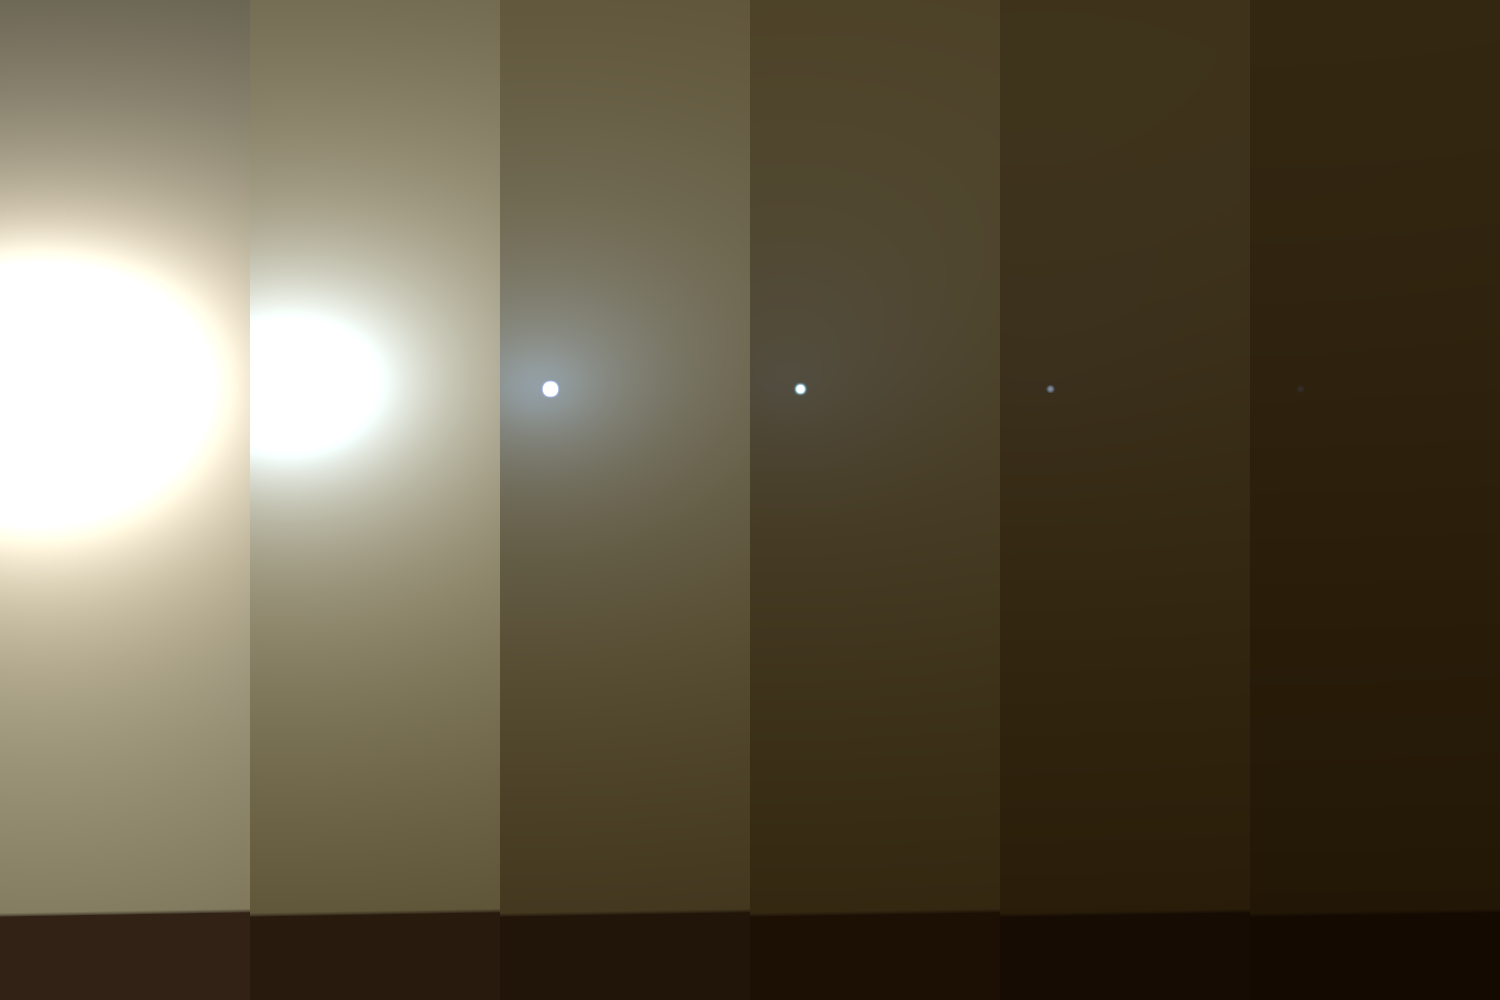
\includegraphics[width=0.7\linewidth]{sections/mars-solar-energy/solar-radiation/images/tau-factors.png}\\
  \caption[Simulated views of atmospheric dust opacity for varying $\tau$ factors]
          {Simulated views of atmospheric dust opacity for varying $\tau$ factors. From left to right frames, tau factors of 1, 3, 5, 7, 9, and 11. Credits: NASA/JPL-Caltech/TAMU.}
  \label{fig:image:tau-factors}
\end{figure}

\subsubsection{Storms}
\label{sec:MartianEnvironment:Dust:Storms}

Dust storms are likely to occur while Mars approaches the Sun during the periphelion season between $L_{s} = \SI{185}{\degree}$ and $L_{s} = \SI{315}{\degree}$ \citemarsenv{Smith2019}. The Sun's proximity warms the atmosphere which creates temperature differences that produce dust lifting winds. The process is exacerbated by the release of carbon dioxide from the evaporating winter polar cap which thickens the atmosphere and increases surface pressure so that dust particles remain airborn. Figure \ref{fig:image:global-dust-storm-timing} shows the the timing of global dust storms until \ac{MY} 34.

\begin{figure}[h]
  \centering
  \hypersetup{linkcolor=captionTextColor}
  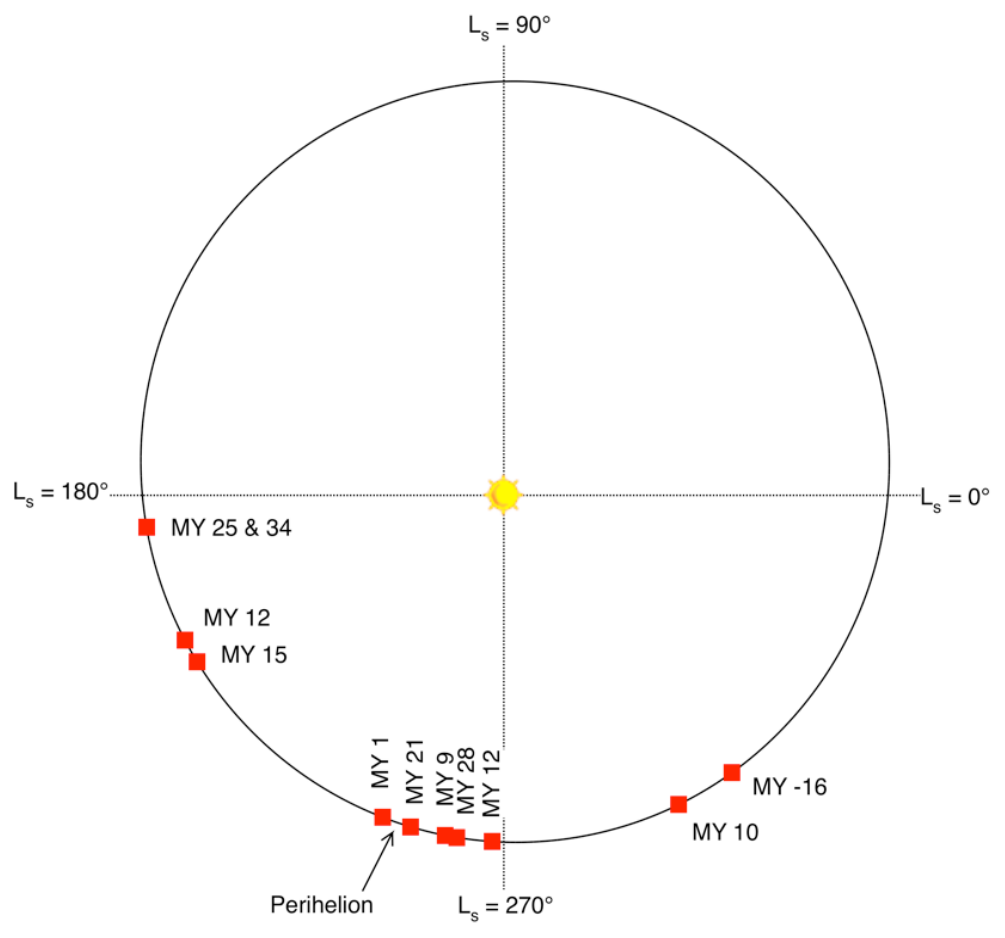
\includegraphics[width=0.4\linewidth]{sections/mars-solar-energy/solar-radiation/images/timin-of-observed-global-dust-storms.png}\\
  \caption[Timing of observed global dust storms on Mars]
          {Timing of observed global dust storms on Mars is concentrated in the season near the periphelion. Taken from \citemarsenv{Smith2019}.}
  \label{fig:image:global-dust-storm-timing}
\end{figure}

Global dust storms that cover an area of over \SI{e7}{\kilo\meter\squared} have a yearly probability of \SI{30}{\percent} to \SI{80}{\percent} whereas local dust storms that cover an area less than \SI{e7}{\kilo\meter\squared} occur with a \SI{5}{\percent} probability \citepower{Kerslake1999}. Local dust storms typically have a $\tau$ factor of approximately 1 \citepower{Kerslake1999} whereas the largest in situ $\tau$ factor recorded by \ac{MER} Opportunity was 10.8 in \ac{MY}34 near $L_{s} = \SI{180}{\degree}$.


\subsection{Solar Radiation}
\label{sec:MartianEnvironment:SolarRadiation}

\todo[inline]{\textbf{TODO:} Short introduction on Solar Radiation.}

The radiation profiles illustrated in this section with respect to Martian surface are for MER Opportunity's final location at Endeavour Crater. Calculations presented in this section as well their nomenclatures are taken from \citemarsenv{Appelbaum1989}, \citemarsenv{Appelbaum1990}, \citemarsenv{Appelbaum1991}, \citemarsenv{Appelbaum1993}, and \citemarsenv{Appelbaum1994} where profiles at locations of \ac{VL1} and \ac{VL2} can be observed.

\subsubsection{Irradiance}
\label{sec:MartianEnvironment:SolarRadiation:Irradiance}

Beam irradiance is the total solar flux density expressed in \si{Wm^{-2}}. It is a measure of solar radiation from direct sunlight. At the top of the Martian atmosphere the instantaneous beam irradiance, $G_{ob}$, is a function the areocentric longitude $L_{s}$:

\begin{equation}
  \label{eq:G_ob}
  G_{ob} = 590 \frac{[1 + e \cos{(Ls - 248)}]^2}{(1-e^2)^2}
\end{equation}

Where \SI{590}{Wm^{-2}} is the mean beam irradiance at the top of the Martian atmosphere, $L_{s} - \SI{248}{\degree}$ is the true anomaly, and $e$ is the Mars eccentricity. The variation of $G_{ob}$ is presented in Figure \ref{fig:plot:beam-irradiance-top-of-mars-atmosphere}. At its closest, the perihelion, Mars is at a distance of \SI{1.381}{\astronomicalunit} from the Sun with a beam irradiance on top of its atmosphere reaching its maximum of \SI{718}{Wm^{-2}} at $L_{s} = \SI{248}{\degree}$. At its furthest of \SI{1.666}{\astronomicalunit}, the aphelion, beam irradiance reaches its minimum of \SI{494}{Wm^{-2}} at $L_{s} = \SI{71}{\degree}$.

\begin{figure}[H]
  \centering
  \hypersetup{linkcolor=captionTextColor}
  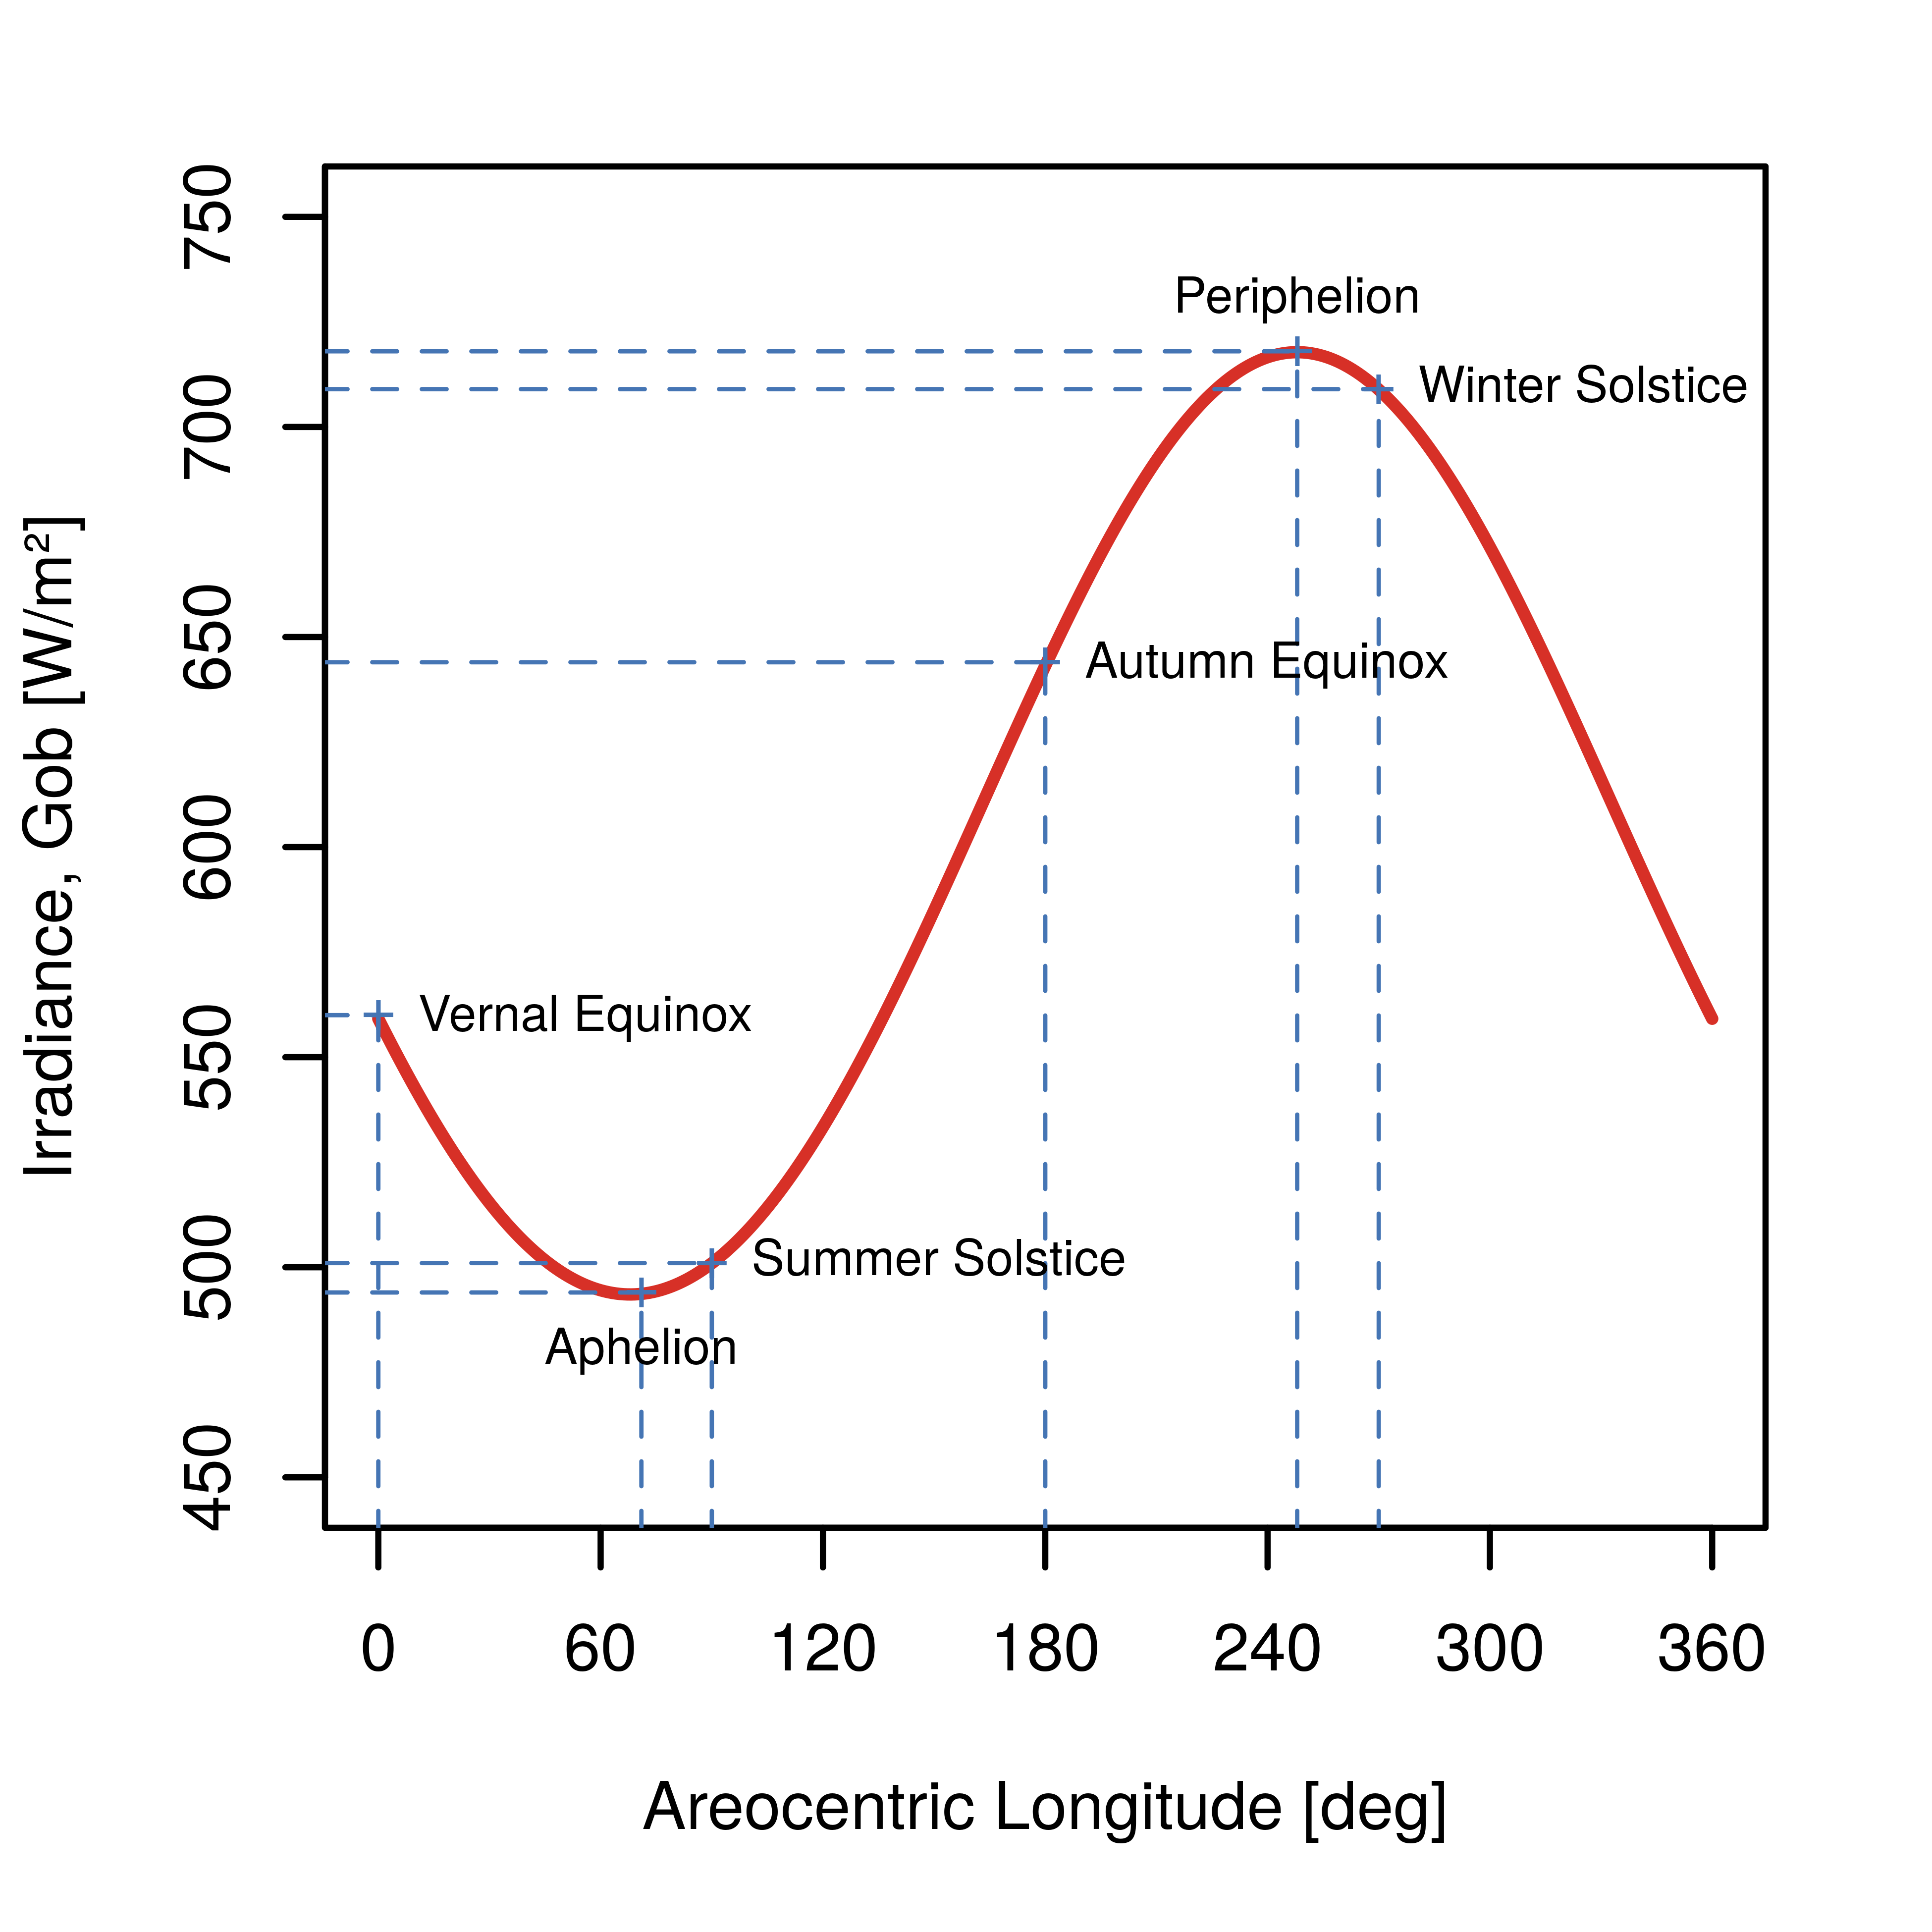
\includegraphics[width=0.5\linewidth]{sections/mars-solar-energy/solar-radiation/plots/gob-daily-variations.png}\\
  \caption[Beam irradiance at top of Mars atmosphere as a function of Areocentric Longitude]
          {Beam irradiance at top of Mars atmosphere as a function of Areocentric Longitude}
  \label{fig:plot:beam-irradiance-top-of-mars-atmosphere}
\end{figure}

Further parameterization becomes necessary in order to measure beam irradiance on a horizontal surface at the top Mars atmosphere where the solar zenith angle $z$ must be considered. The solar zenith angle itself is a function of planetary latitude $\phi$, declination angle $\delta$, and hour angle $\omega$ measured from the true noon westward \citemarsenv{Appelbaum1990}. Expressed as $G_{obh}$, it is presented in Equation \ref{eq:G_obh}:

\begin{equation}
  \label{eq:G_obh}
  G_{obh} = G_{ob}\cos{z}
\end{equation}

where $z$ is given by:

\begin{equation}
  \label{eq:cosz}
  \cos{z} = \sin{\phi}\sin{\delta} + \cos{\phi}\cos{\delta}\cos{\omega}
\end{equation}

Solar radiation calculations using Equation \ref{eq:G_obh} as a function of Solar time are presented in Figure \ref{fig:plot:diurnal-variation-of-beam-irradiance-on-a-horizontal-surface-at-top-of-mars-atmosphere}.

\begin{figure}[h]
  \centering
  \hypersetup{linkcolor=captionTextColor}
  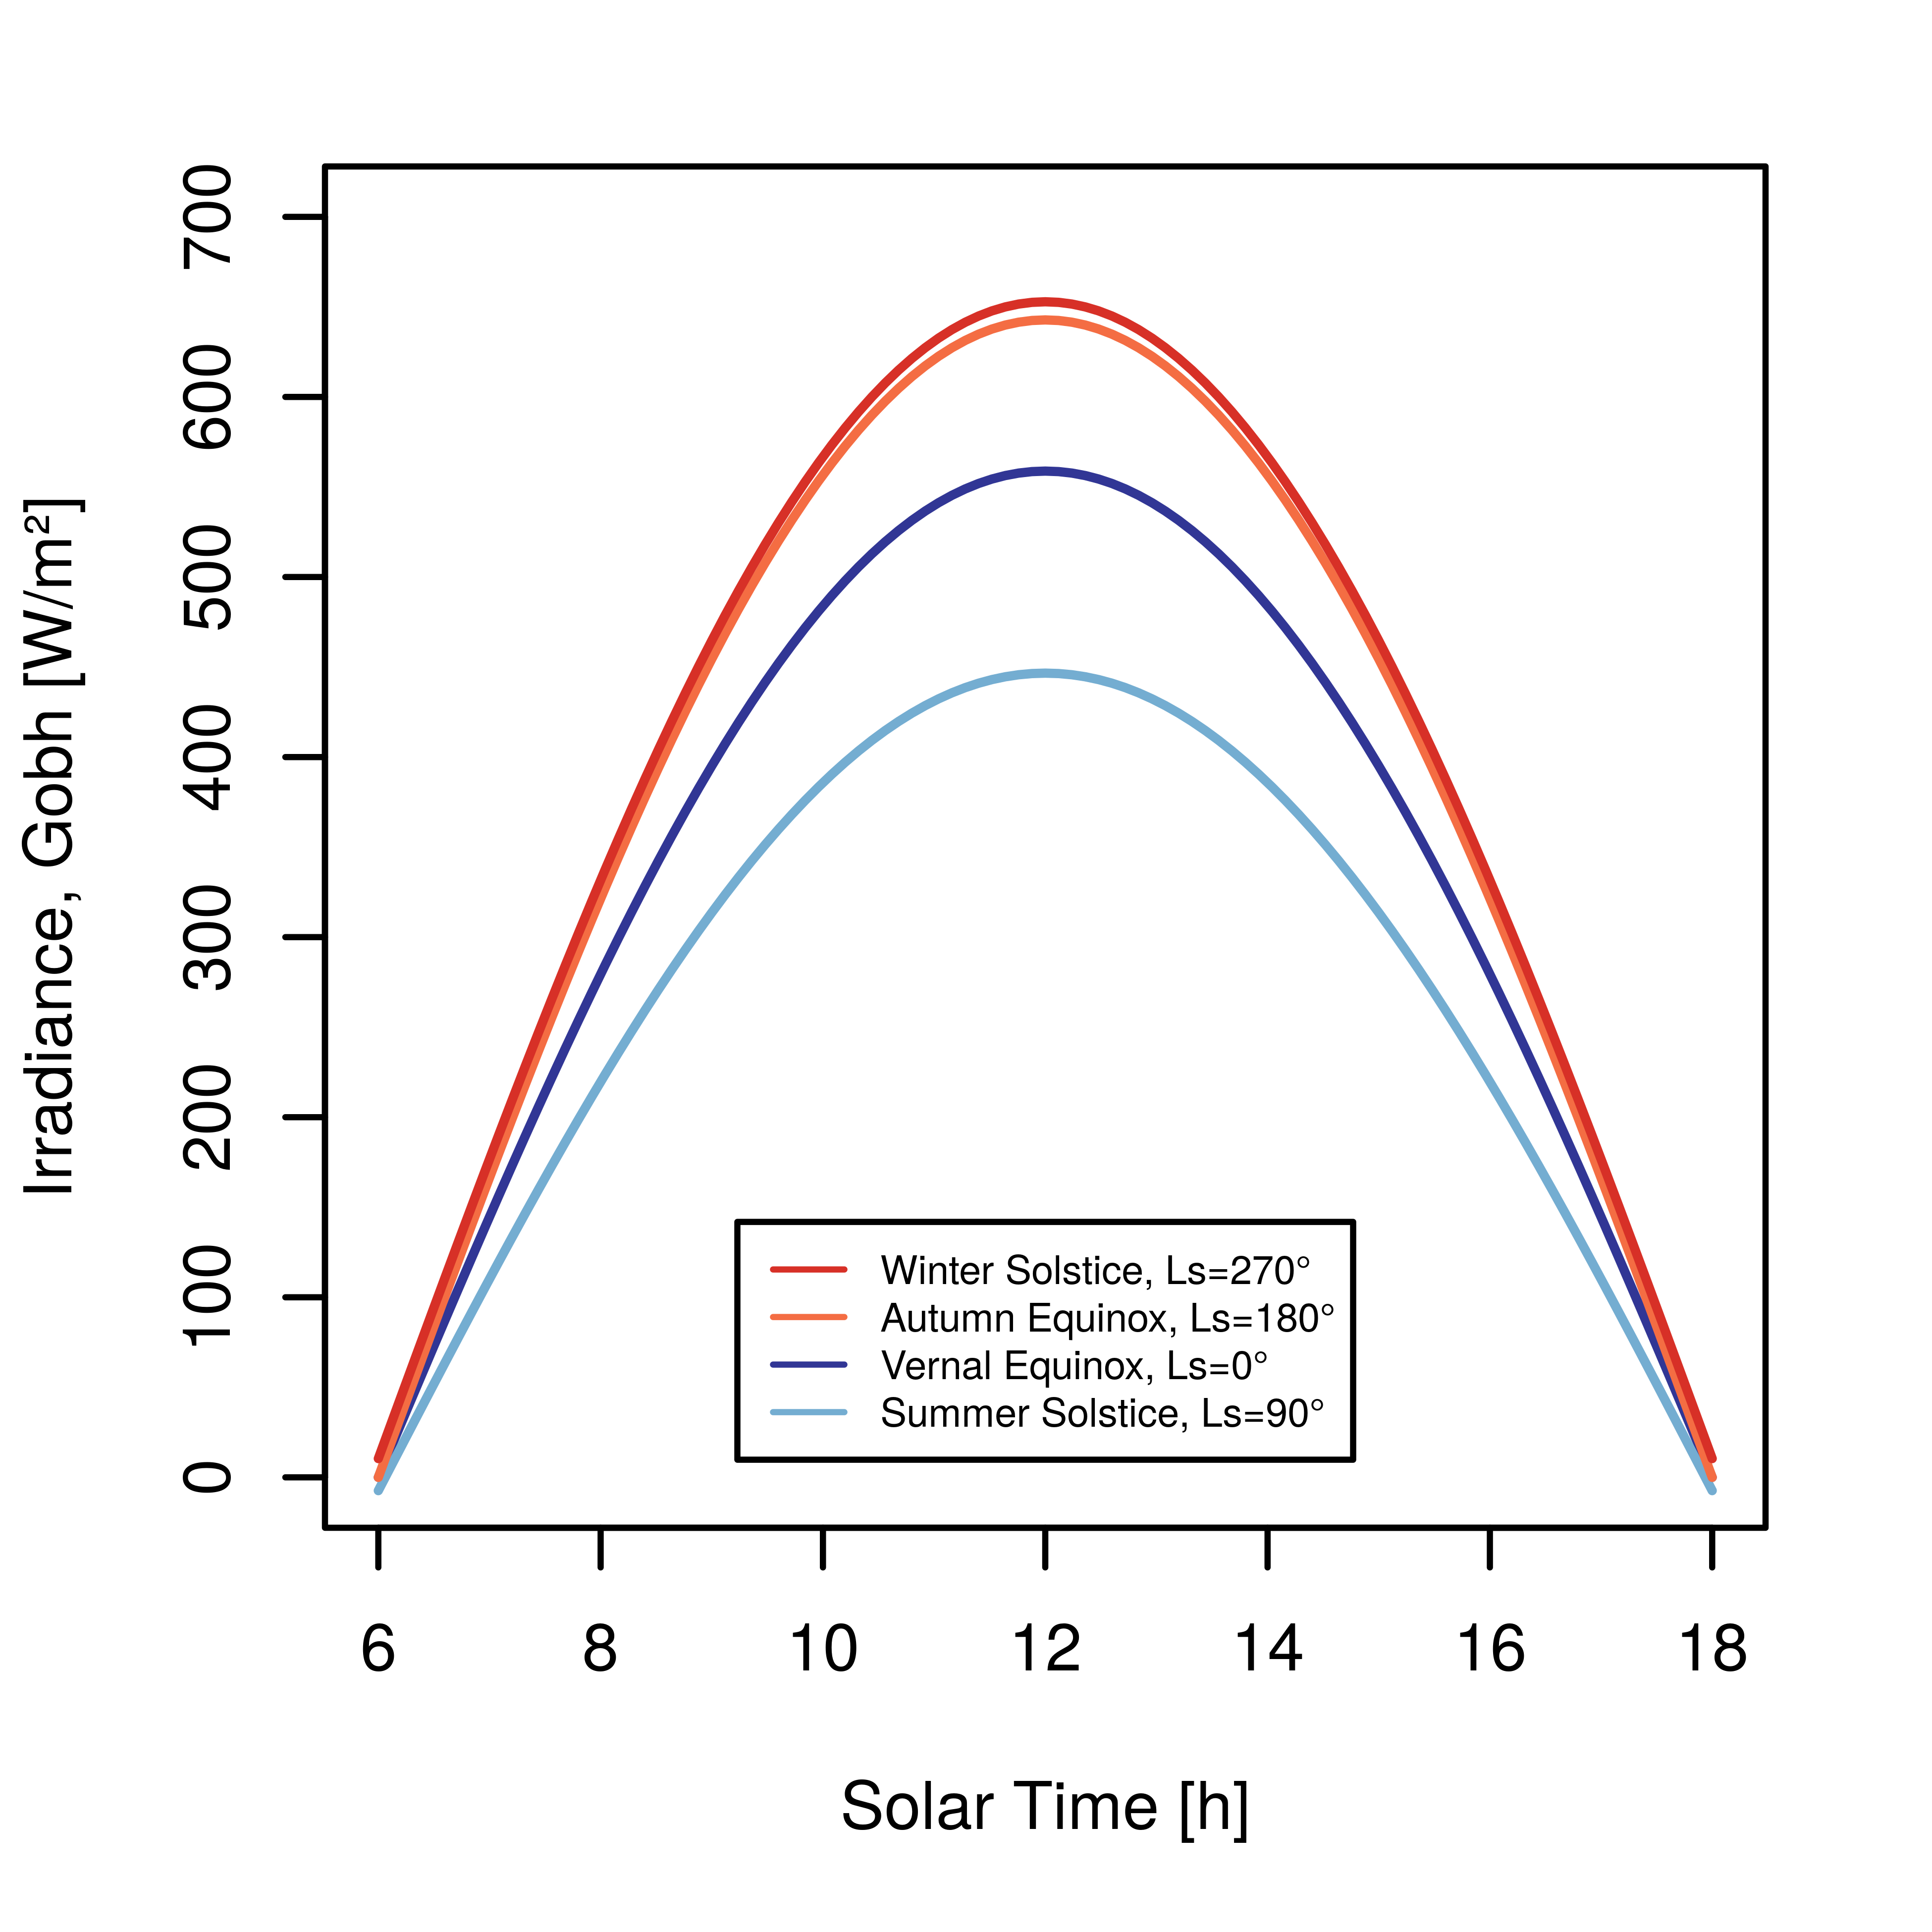
\includegraphics[width=0.5\linewidth]{sections/mars-solar-energy/solar-radiation/plots/gobh-diurnal-over-endaveaour-crater.png}\\
  \caption[Diurnal variation of beam irradiance on a horizontal surface at top of Mars atmosphere above Endaveaour Crater]
  {Diurnal variation of beam irradiance on a horizontal surface at top of Mars atmosphere above Endaveaour Crater.}
  \label{fig:plot:diurnal-variation-of-beam-irradiance-on-a-horizontal-surface-at-top-of-mars-atmosphere}
\end{figure}

Obtaining the irradiance on the surface of Mars requires the atmospheric opacity $\tau$ as an additional parameter. A distinction exists between global, direct, and diffuse beam irradiance where global beam irradiance $G_{h}$ is the sum of direct, $G_{bh}$, and diffuse beam irradiances, $G_{dh}$:

\todo[inline]{\textbf{TODO:} Explain scattering and diffuse irradiance.}

% TOOD: Mention scattering: https://ntrs.nasa.gov/archive/nasa/casi.ntrs.nasa.gov/20040191326.pdf

\begin{equation}
  \label{eq:G_h_1}
  G_{h} = G_{bh} + G_{dh}
\end{equation}

The expression for $G_{h}$ and $G_{bh}$ are presented in Equations \ref{eq:G_h} and \ref{eq:G_bh}:

\begin{equation}
  \label{eq:G_h_2}
  G_{h} = G_{ob}\cos{z}\frac{f(z,\tau)}{0.9}
\end{equation}

where $f(z,\tau)$ is the normalized net flux function derived from the net solar flux integrated over the solar spectrum on the Martian surface and 0.9 comes from the $(1-albedo)$ expression for an albedo of 0.1 \citemarsenv{Appelbaum1989}.

\begin{equation}
  \label{eq:G_bh}
  G_{bh} = G_{ob}\cos{z}\exp\left(\frac{-\tau}{cos{z}}\right)
\end{equation}

Diurnal irradiance profiles at Endaveour Crater are presented in Figure \ref{fig:plot:irradiances-phi} for different planetary latitudes during the perihelion. At $L_{s} = \SI{248}{\degree}$ the northern hemisphere is in mid-Autumn whereas the southern hemisphere in mid-Spring, as such irradiances are much larger at $\phi = \SI{-40}{\degree}$ and $\phi = \SI{-20}{\degree}$ than they are at $\phi = \SI{0}{\degree}$ and $\phi = \SI{40}{\degree}$.

\begin{figure}[h]
\captionsetup[subfigure]{justification=centering}
\vspace{-2ex}
	\centering
    %% setup sizes
    \setlength{\subfigureWidth}{0.50\textwidth}
    \setlength{\graphicsHeight}{80mm}
    %% kill hyper-link highlighting
    \hypersetup{hidelinks=true}%
    %% the figures
%% 1st row
  	\begin{subfigure}[t]{\subfigureWidth}
      \centering
  		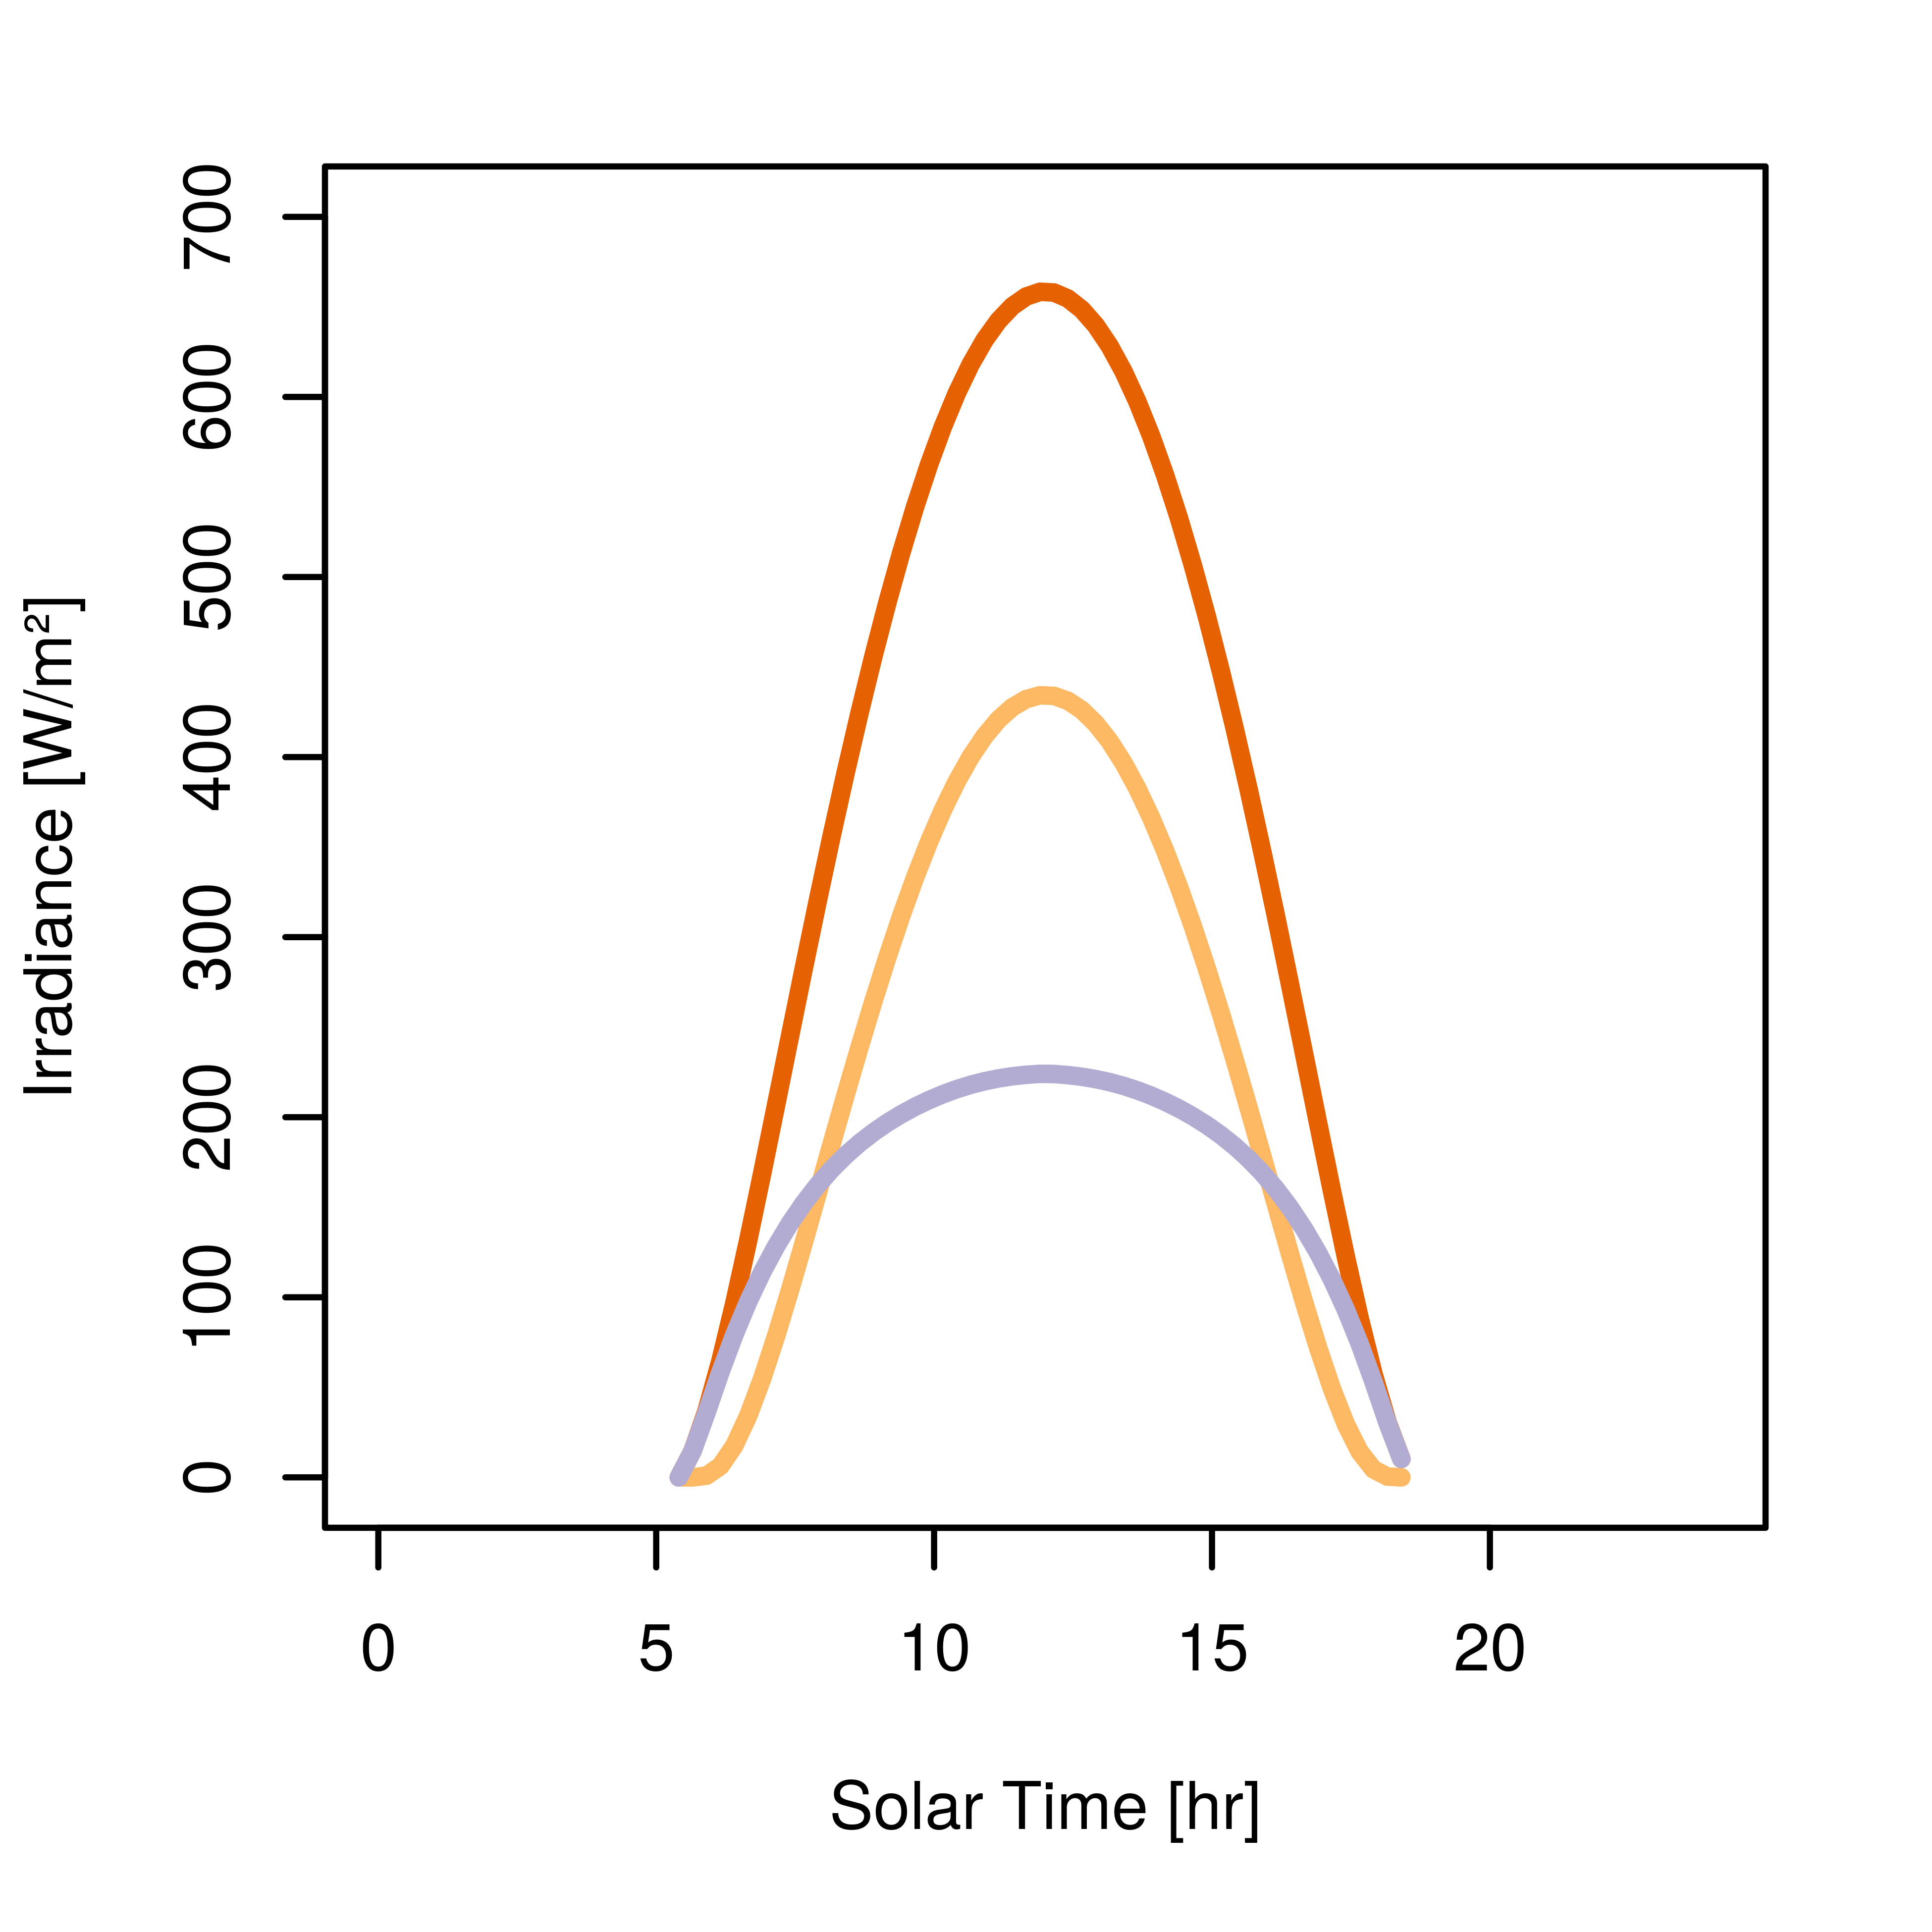
\includegraphics[height=\graphicsHeight]{sections/mars-solar-energy/solar-radiation/plots/gh-gbh-gdh-variation-1-for-ls-248-phi-20-tau-05-and-albedo-027.png}
  		\subcaption{$\phi = \SI{-40}{\degree}$}
  		\label{fig:sub:irradiance-phi-m20}
  	\end{subfigure}\hfill
    \begin{subfigure}[t]{\subfigureWidth}
      \centering
  		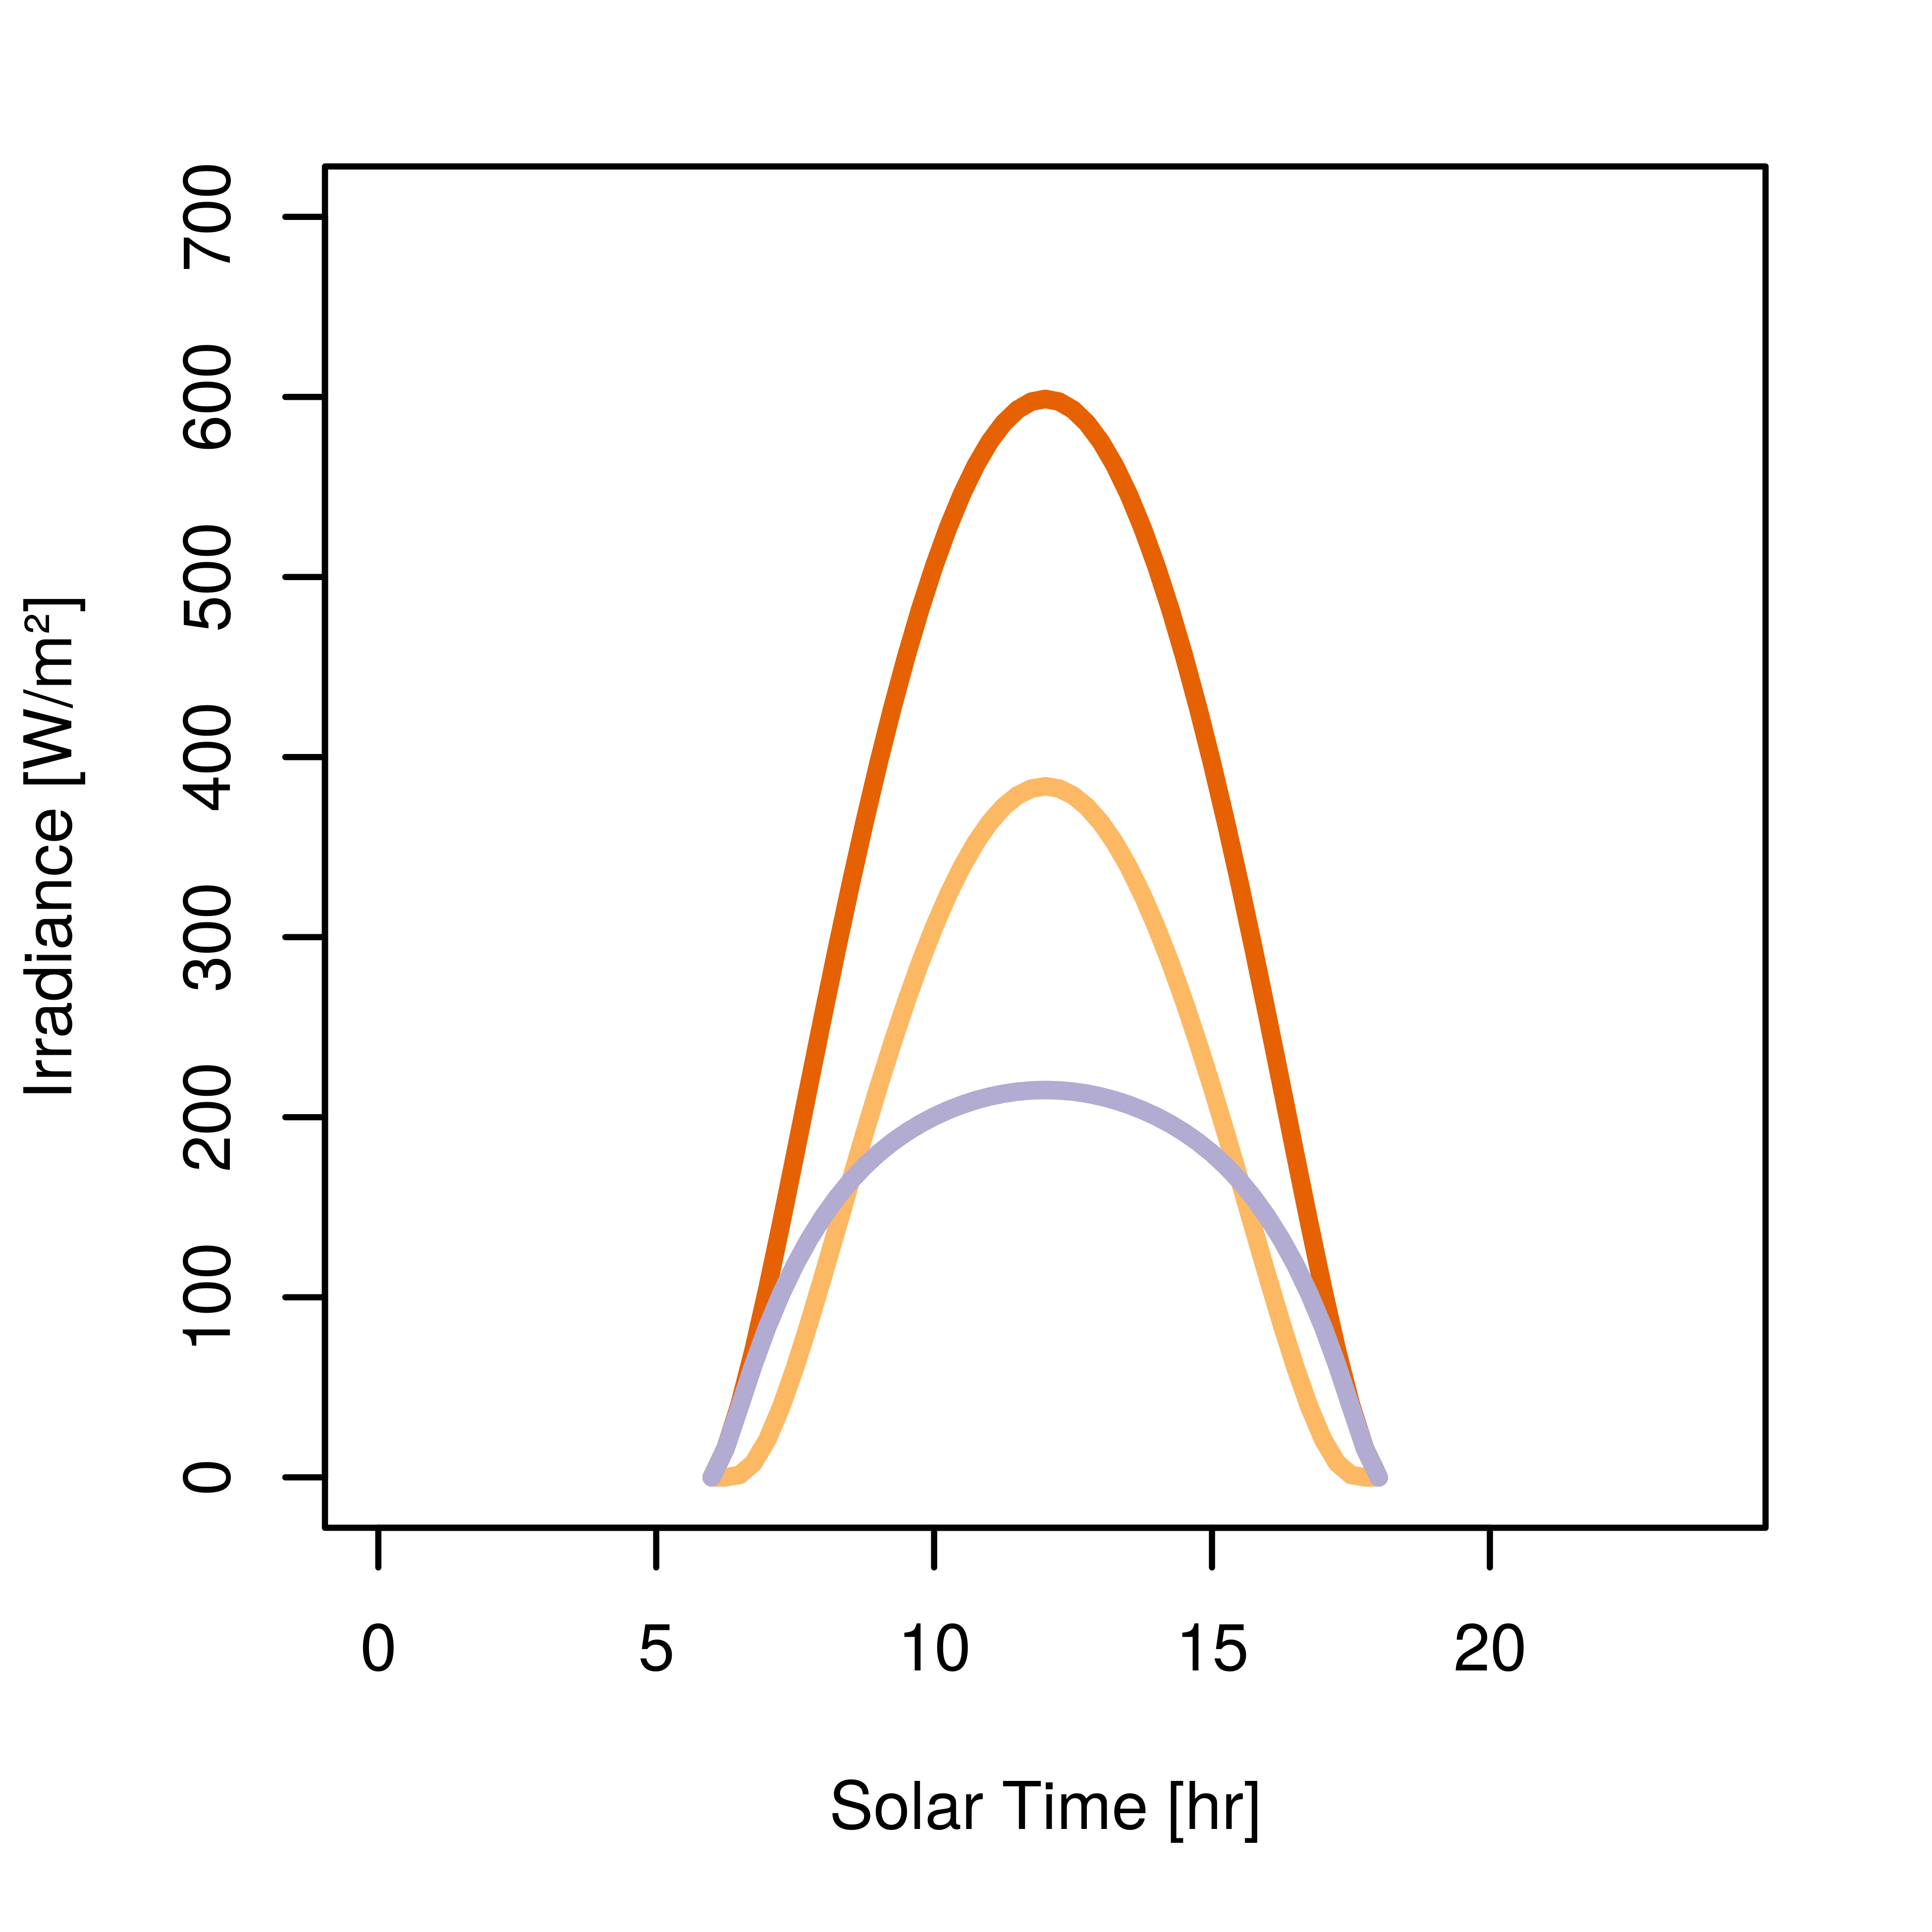
\includegraphics[height=\graphicsHeight]{sections/mars-solar-energy/solar-radiation/plots/gh-gbh-gdh-variation-2-for-ls-248-phi-0-tau-05-and-albedo-027.png}
  		\subcaption{$\phi = \SI{-20}{\degree}$}
  		\label{fig:sub:irradiance-phi-0}
  	\end{subfigure}\\[0.8ex]
%% 2nd row
    \begin{subfigure}[t]{\subfigureWidth}
      \centering
  		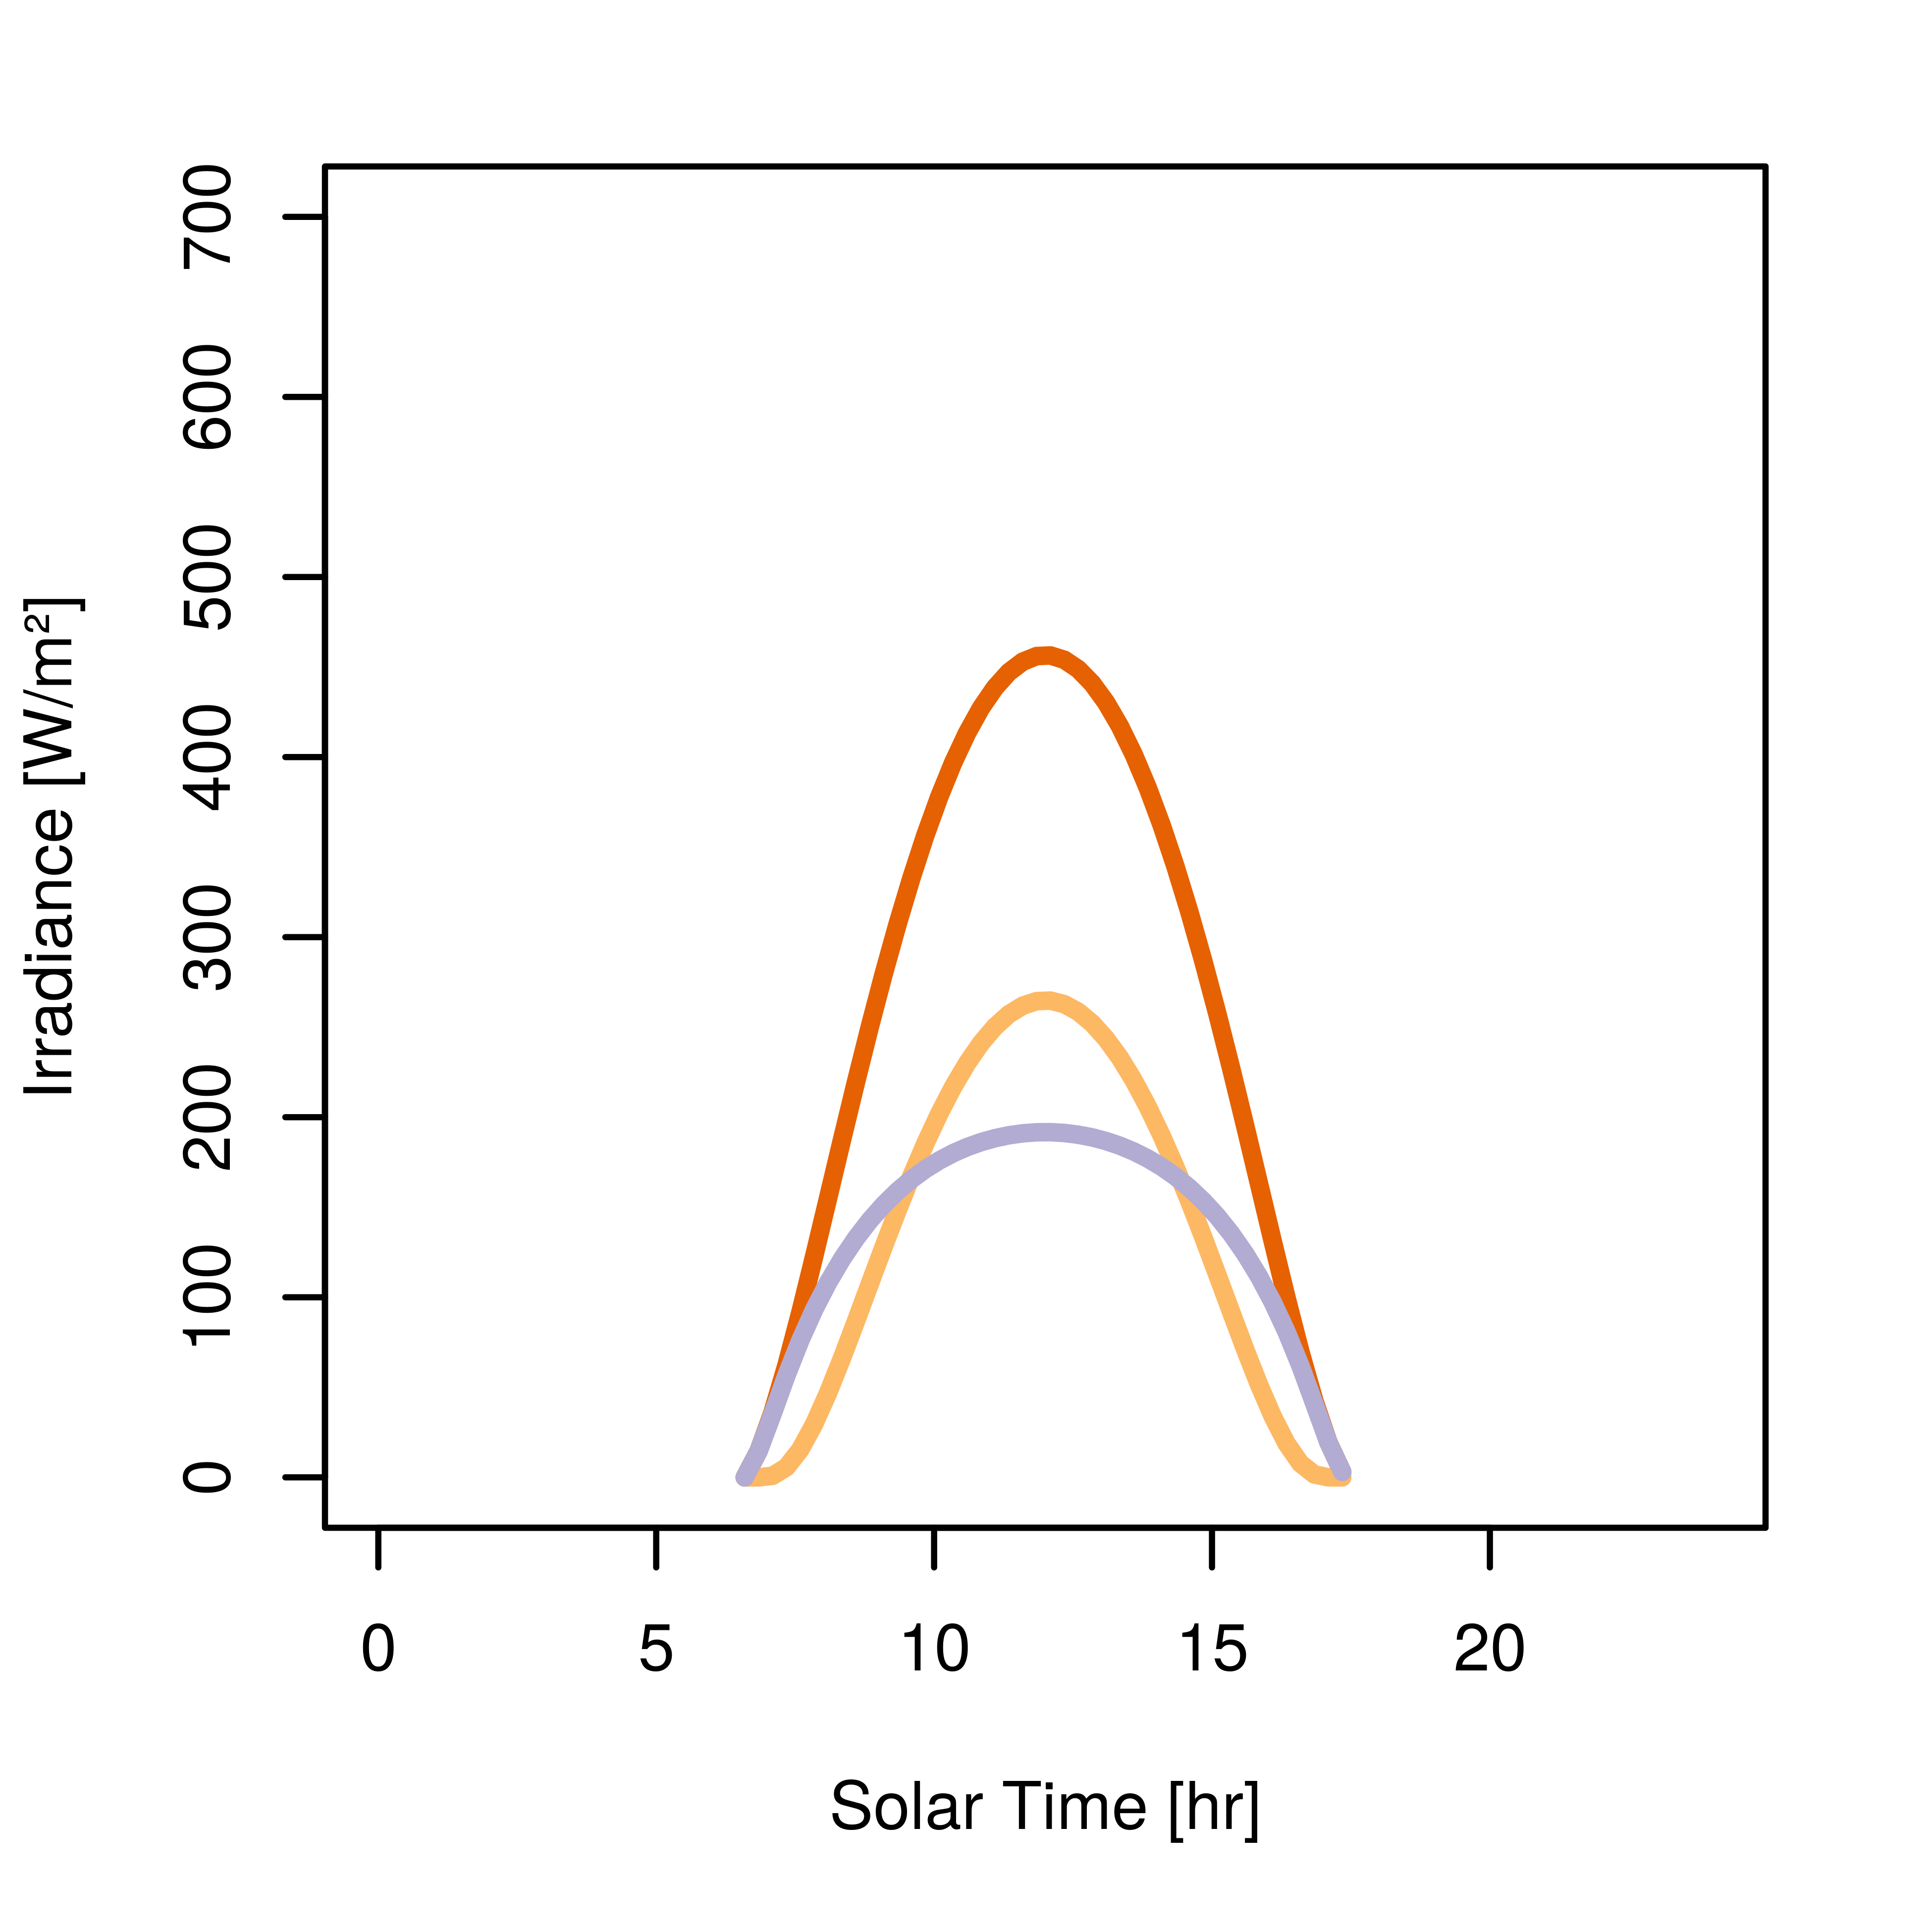
\includegraphics[height=\graphicsHeight]{sections/mars-solar-energy/solar-radiation/plots/gh-gbh-gdh-variation-3-for-ls-248-phi-20-tau-05-and-albedo-027.png}
  		\subcaption{$\phi = \SI{0}{\degree}$}
  		\label{fig:sub:irradiance-phi-p20}
  	\end{subfigure}\hfill
	   \begin{subfigure}[t]{\subfigureWidth}
      \centering
  		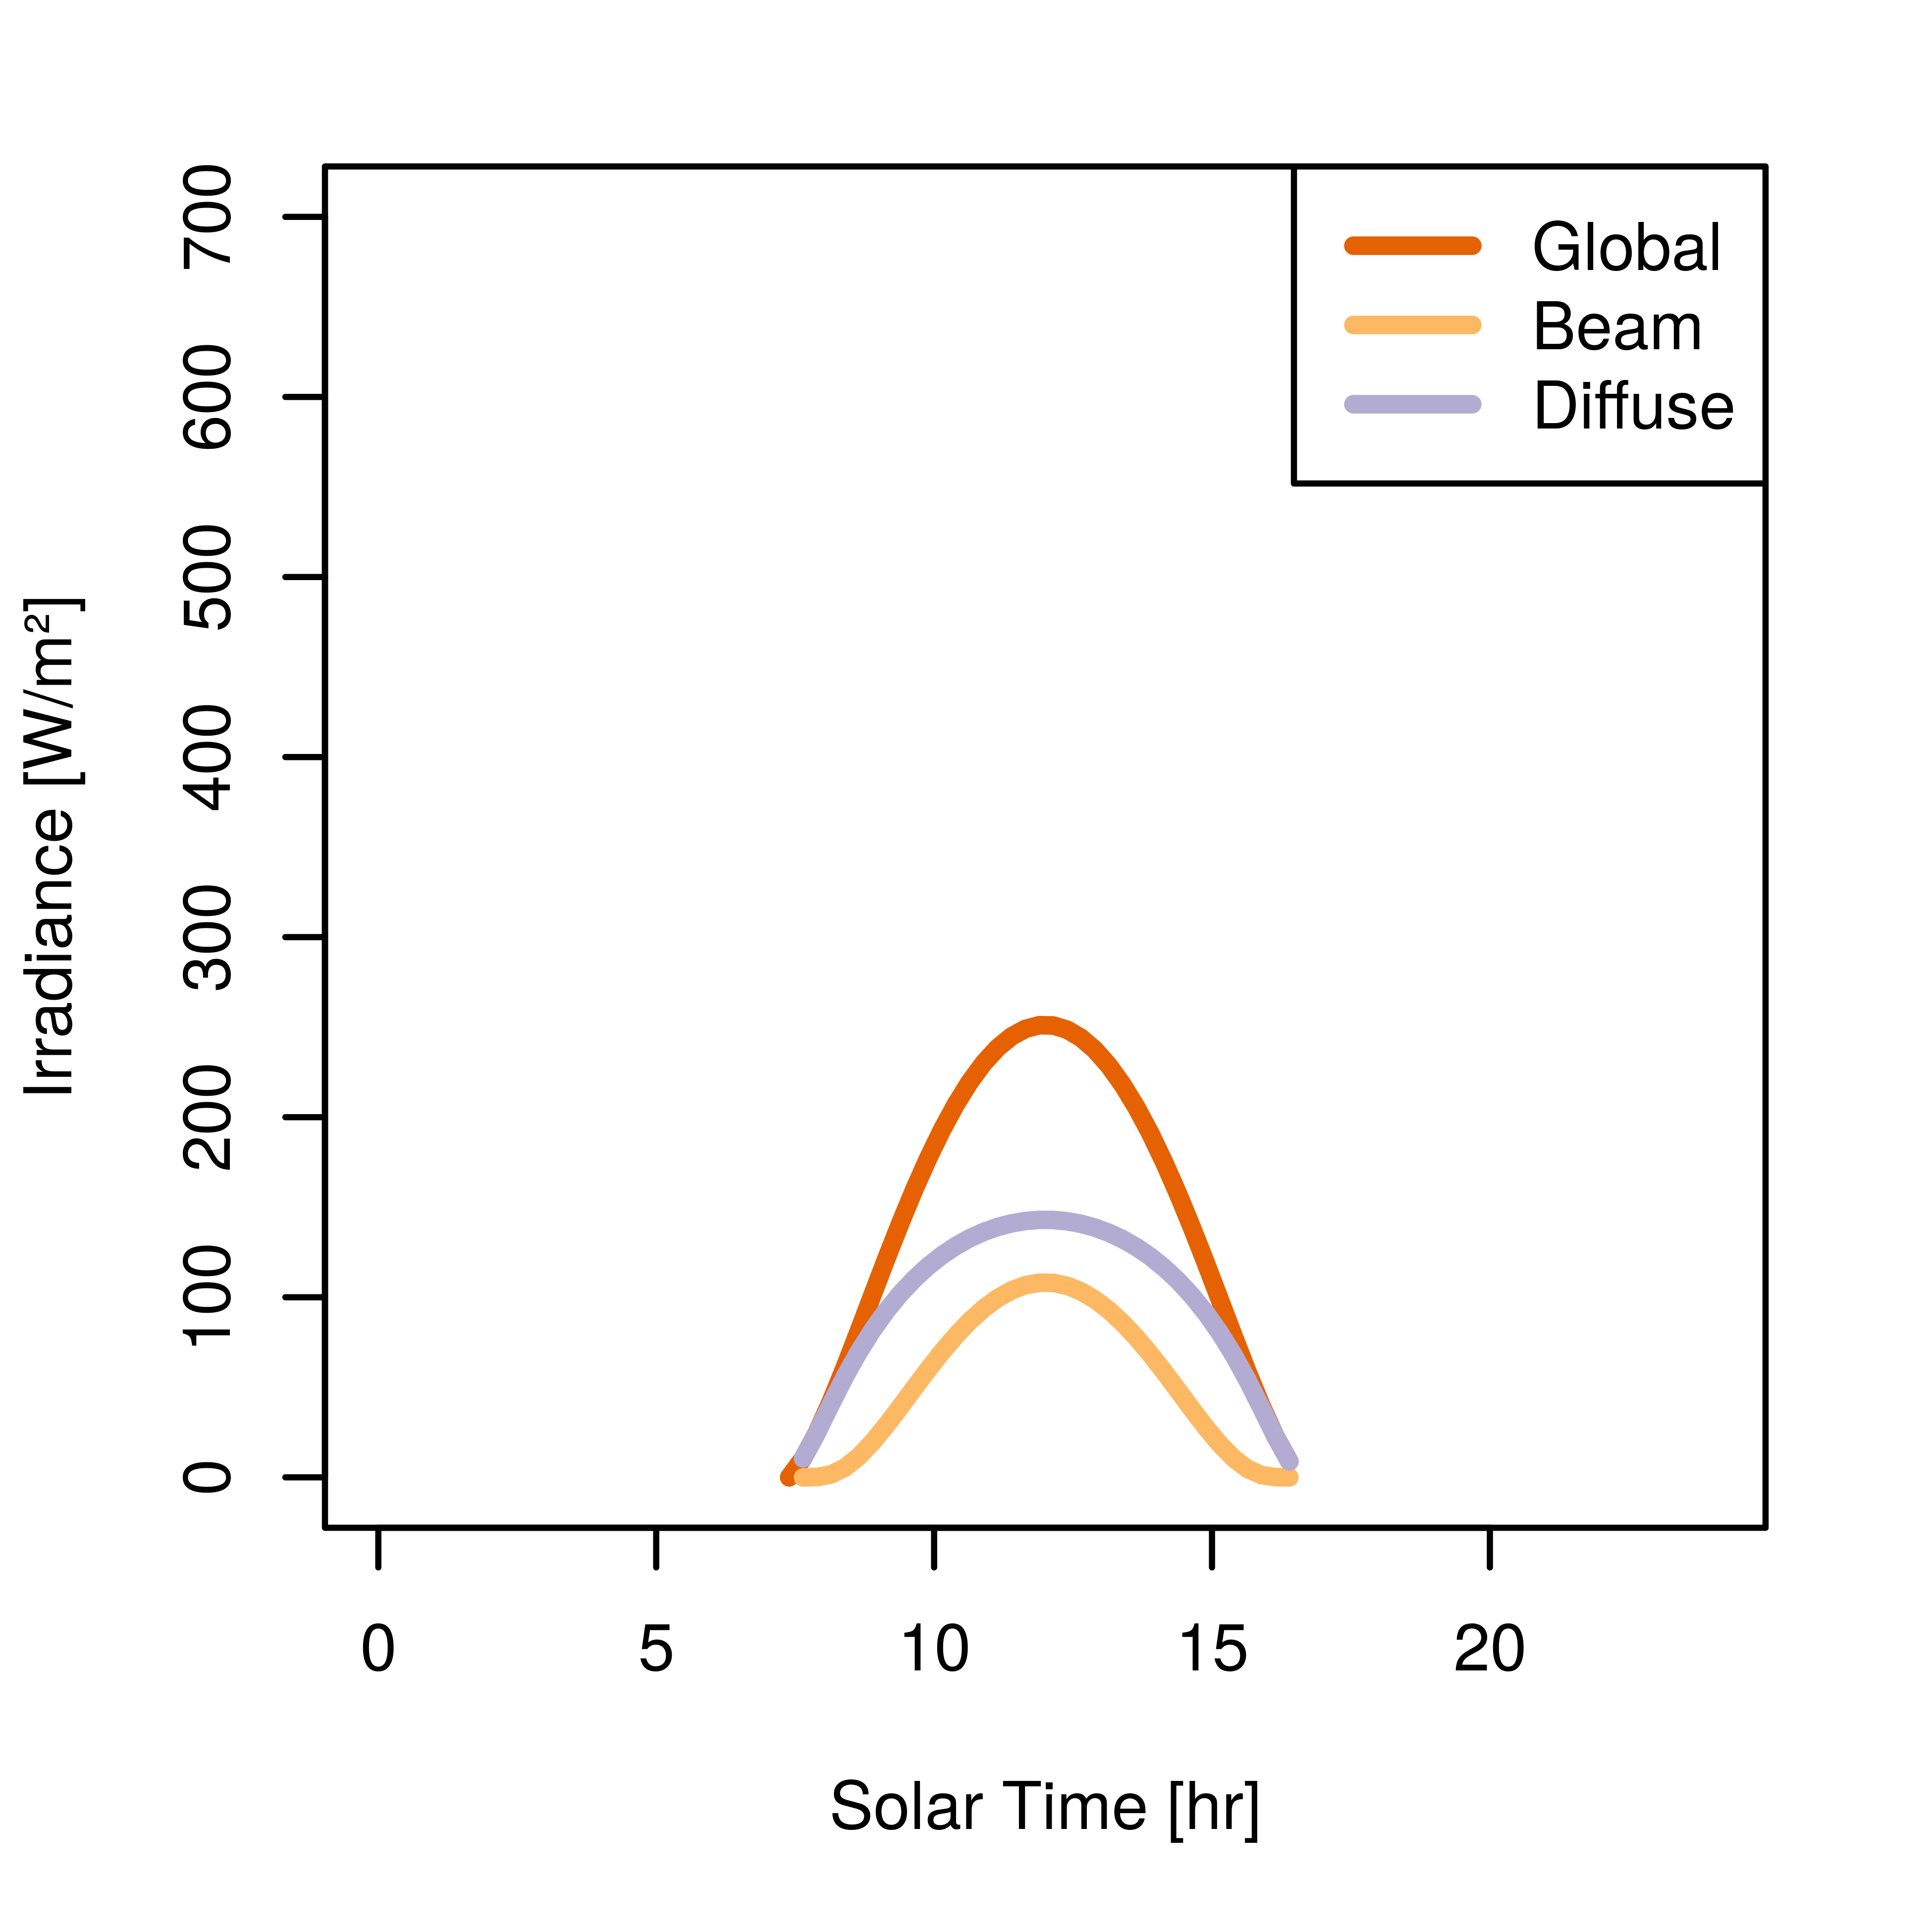
\includegraphics[height=\graphicsHeight]{sections/mars-solar-energy/solar-radiation/plots/gh-gbh-gdh-variation-4-for-ls-248-phi-40-tau-05-and-albedo-027.png}
  		\subcaption{$\phi = \SI{20}{\degree}$}
  		\label{fig:sub:irradiance-phi-p40}
	   \end{subfigure}\hfill
	\caption{Diurnal variation of global, beam, and diffuse irradiance on Mars horizontal surface at different planetary latitudes.}
	\label{fig:plot:irradiances-phi}
\vspace{-2ex}
\end{figure}

\clearpage
\subsubsection{Insolation}
\label{sec:MartianEnvironment:SolarRadiation:Insolation}

Solar insolation is the amount solar radiation incident on a planetary surface during a time period. It is expressed in \si{Whm^{-2}} and obtained by integrating the equations of irradiance over a time period between $\omega_1$ and $\omega_2$. Thus, insolation on a horizontal surface at the top of Mars atmosphere, denoted as $I_{obh}$, is obtained by integrating Equation \ref{eq:G_h_2} of $G_{obh}$.

Global, beam, and diffuse insolations on a horizontal Mars surface are denoted as $I_{h}$, $I_{bh}$, and $I_{dh}$ respectively. Their values are obtained by integrating \ref{eq:G_h_2} for $I_{h}$ and \ref{eq:G_bh} for $I_{bh}$. Diffuse insolation $I_{dh}$ is obtained through the same relationship presented in Equation \ref{eq:G_h_1}. The variation of insolation as a function of $L_{s}$ for different levels of atmospheric opacities are illustrated in Figure \ref{fig:plot:insolation-ls}. Evidently, the insolation curves peak at the perihelion with $L_{s} = \SI{248}{\degree}$ and reach their lowest during the aphelion with $L_{s} = \SI{71}{\degree}$. Due to light scattering by airborn Martian dust \citemarsenv{Merikallio2013}, diffuse insolation is already the largest component contributing to the global insolation at $\tau = 1$. On a dusty day at $\tau = 3$, global insolation is mostly diffuse.

\begin{figure}[h]
\captionsetup[subfigure]{justification=centering}
\vspace{-2ex}
	\centering
    %% setup sizes
    \setlength{\subfigureWidth}{0.50\textwidth}
    \setlength{\graphicsHeight}{80mm}
    %% kill hyper-link highlighting
    \hypersetup{hidelinks=true}%
    %% the figures
%% 1st row
  	\begin{subfigure}[t]{\subfigureWidth}
      \centering
  		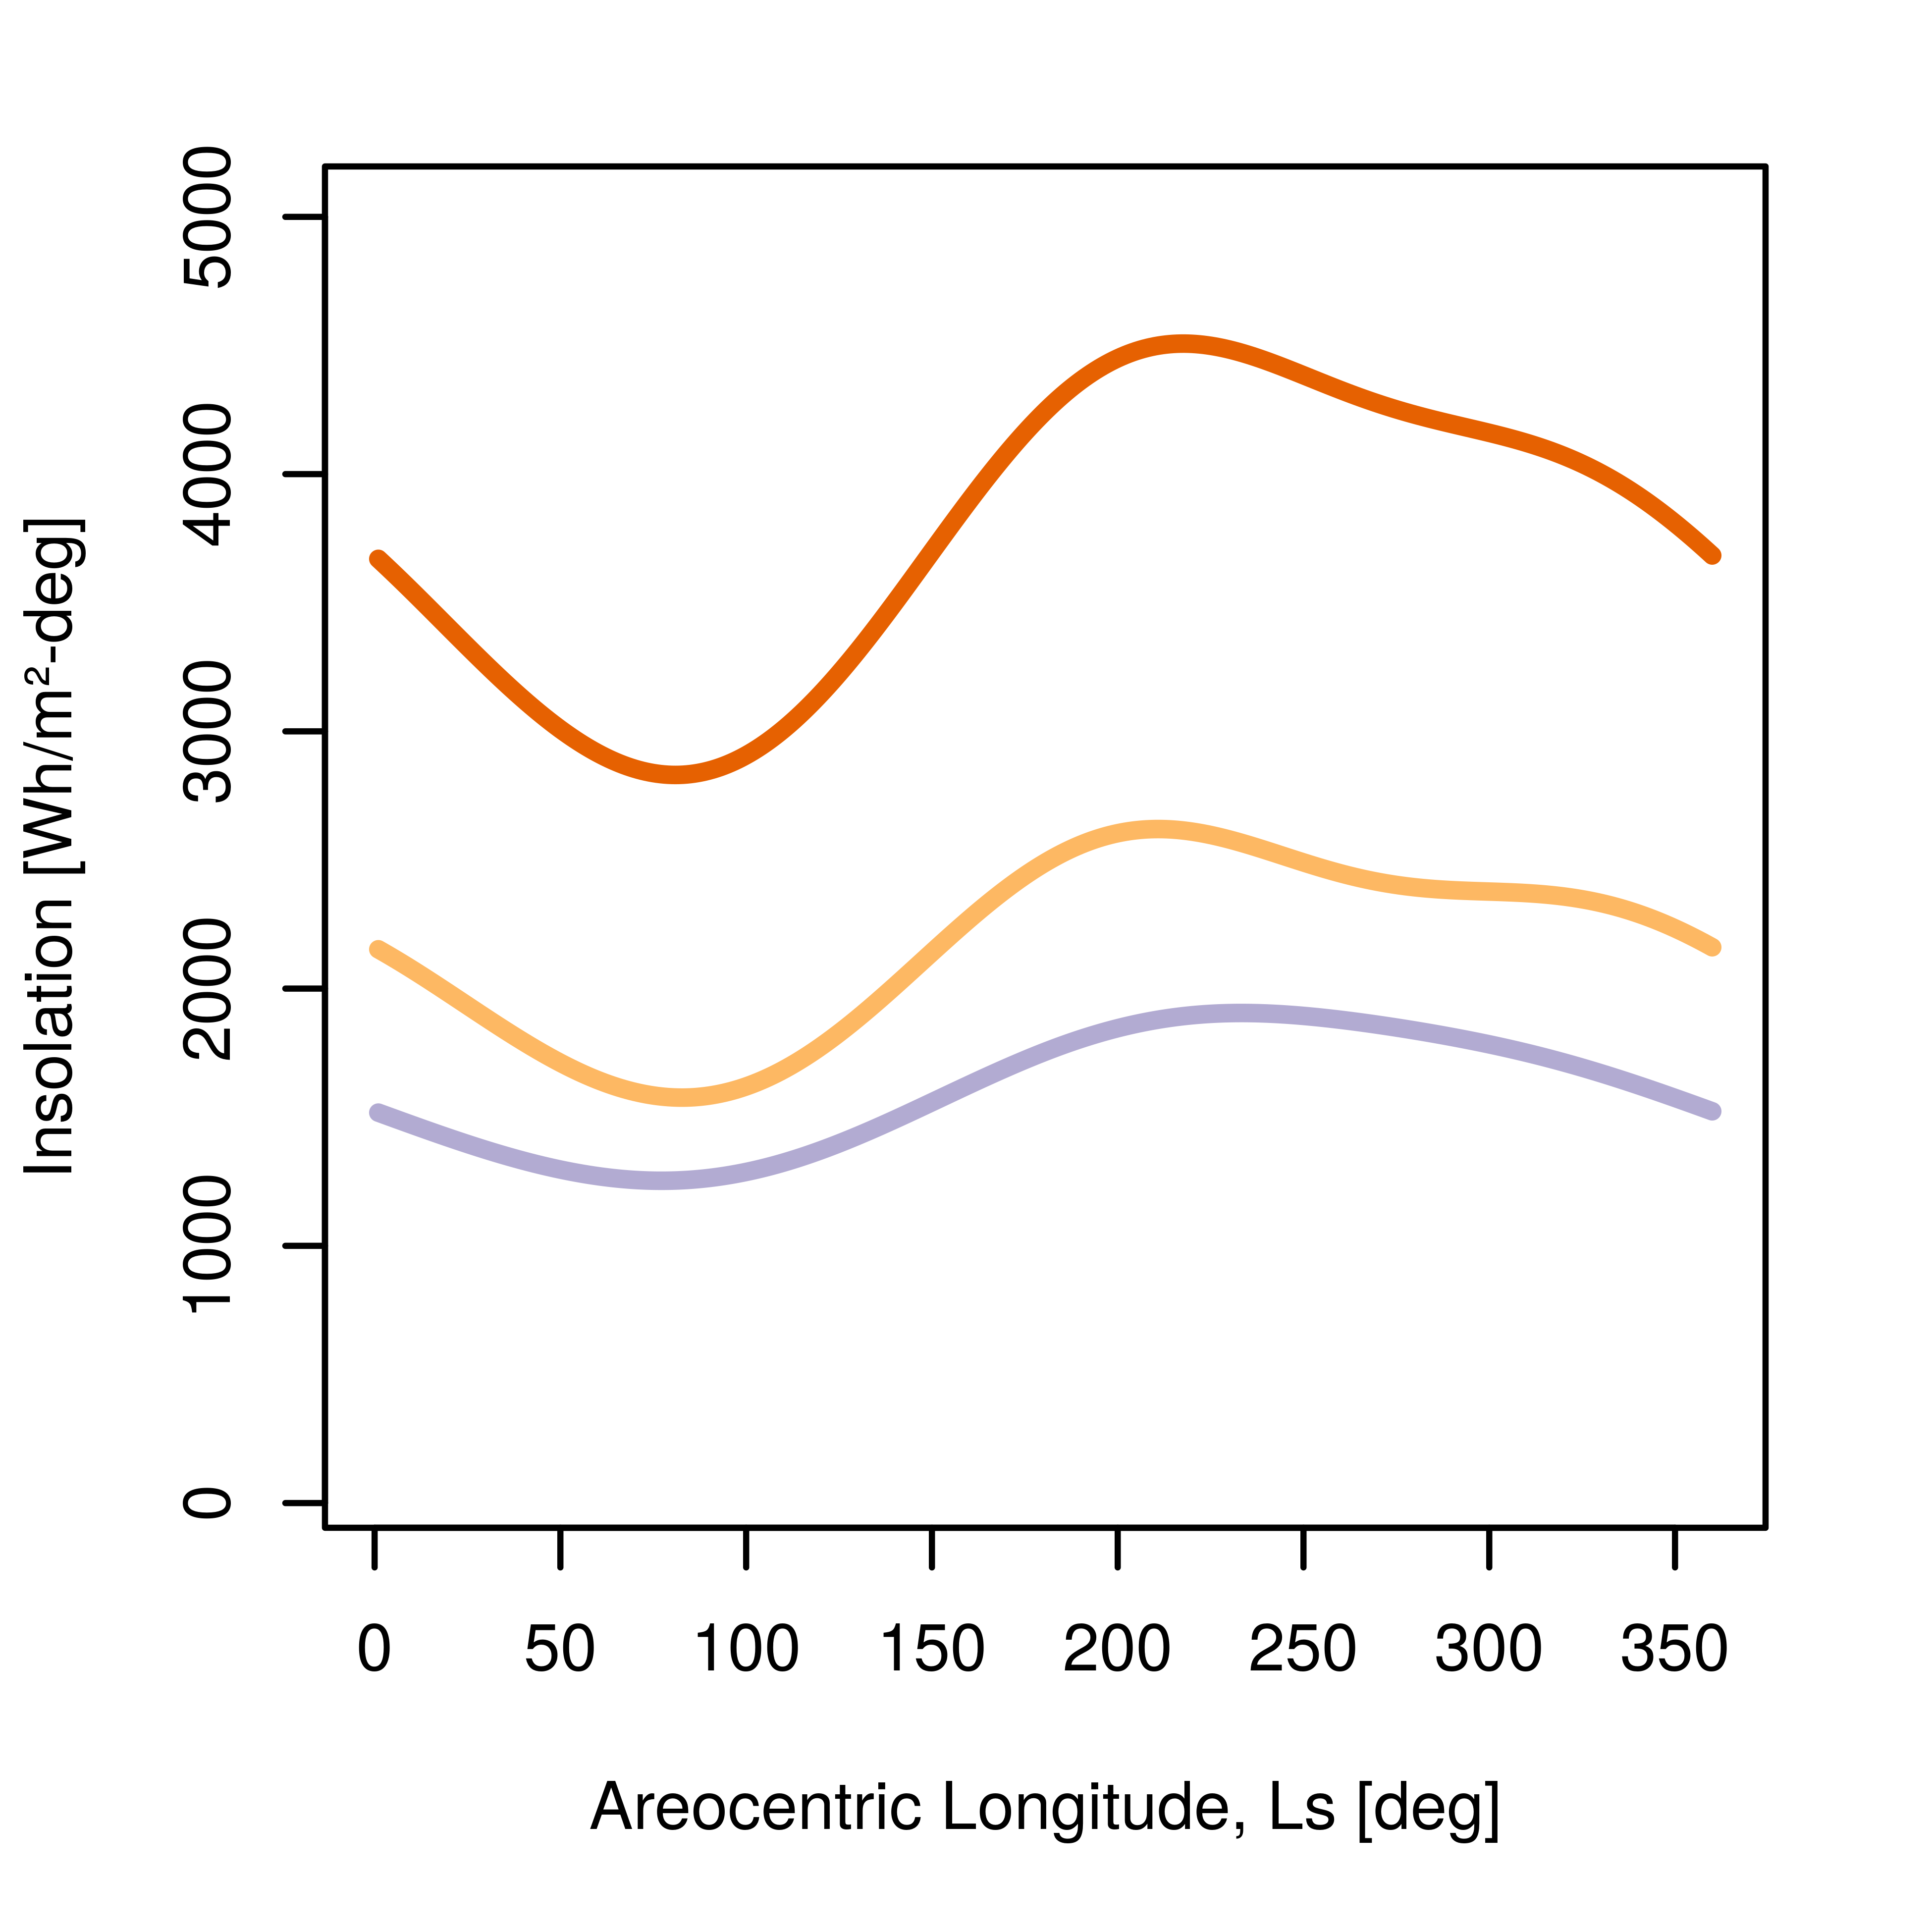
\includegraphics[height=\graphicsHeight]{sections/mars-solar-energy/solar-radiation/plots/hh-hbh-and-hdh-as-a-function-of-ls-for-tau05-phi205-and-albedo-027}
  		\subcaption{$\tau = 0.5$}
  		\label{fig:sub:insolation-ls-tau-factor-0p5}
  	\end{subfigure}\hfill
    \begin{subfigure}[t]{\subfigureWidth}
      \centering
  		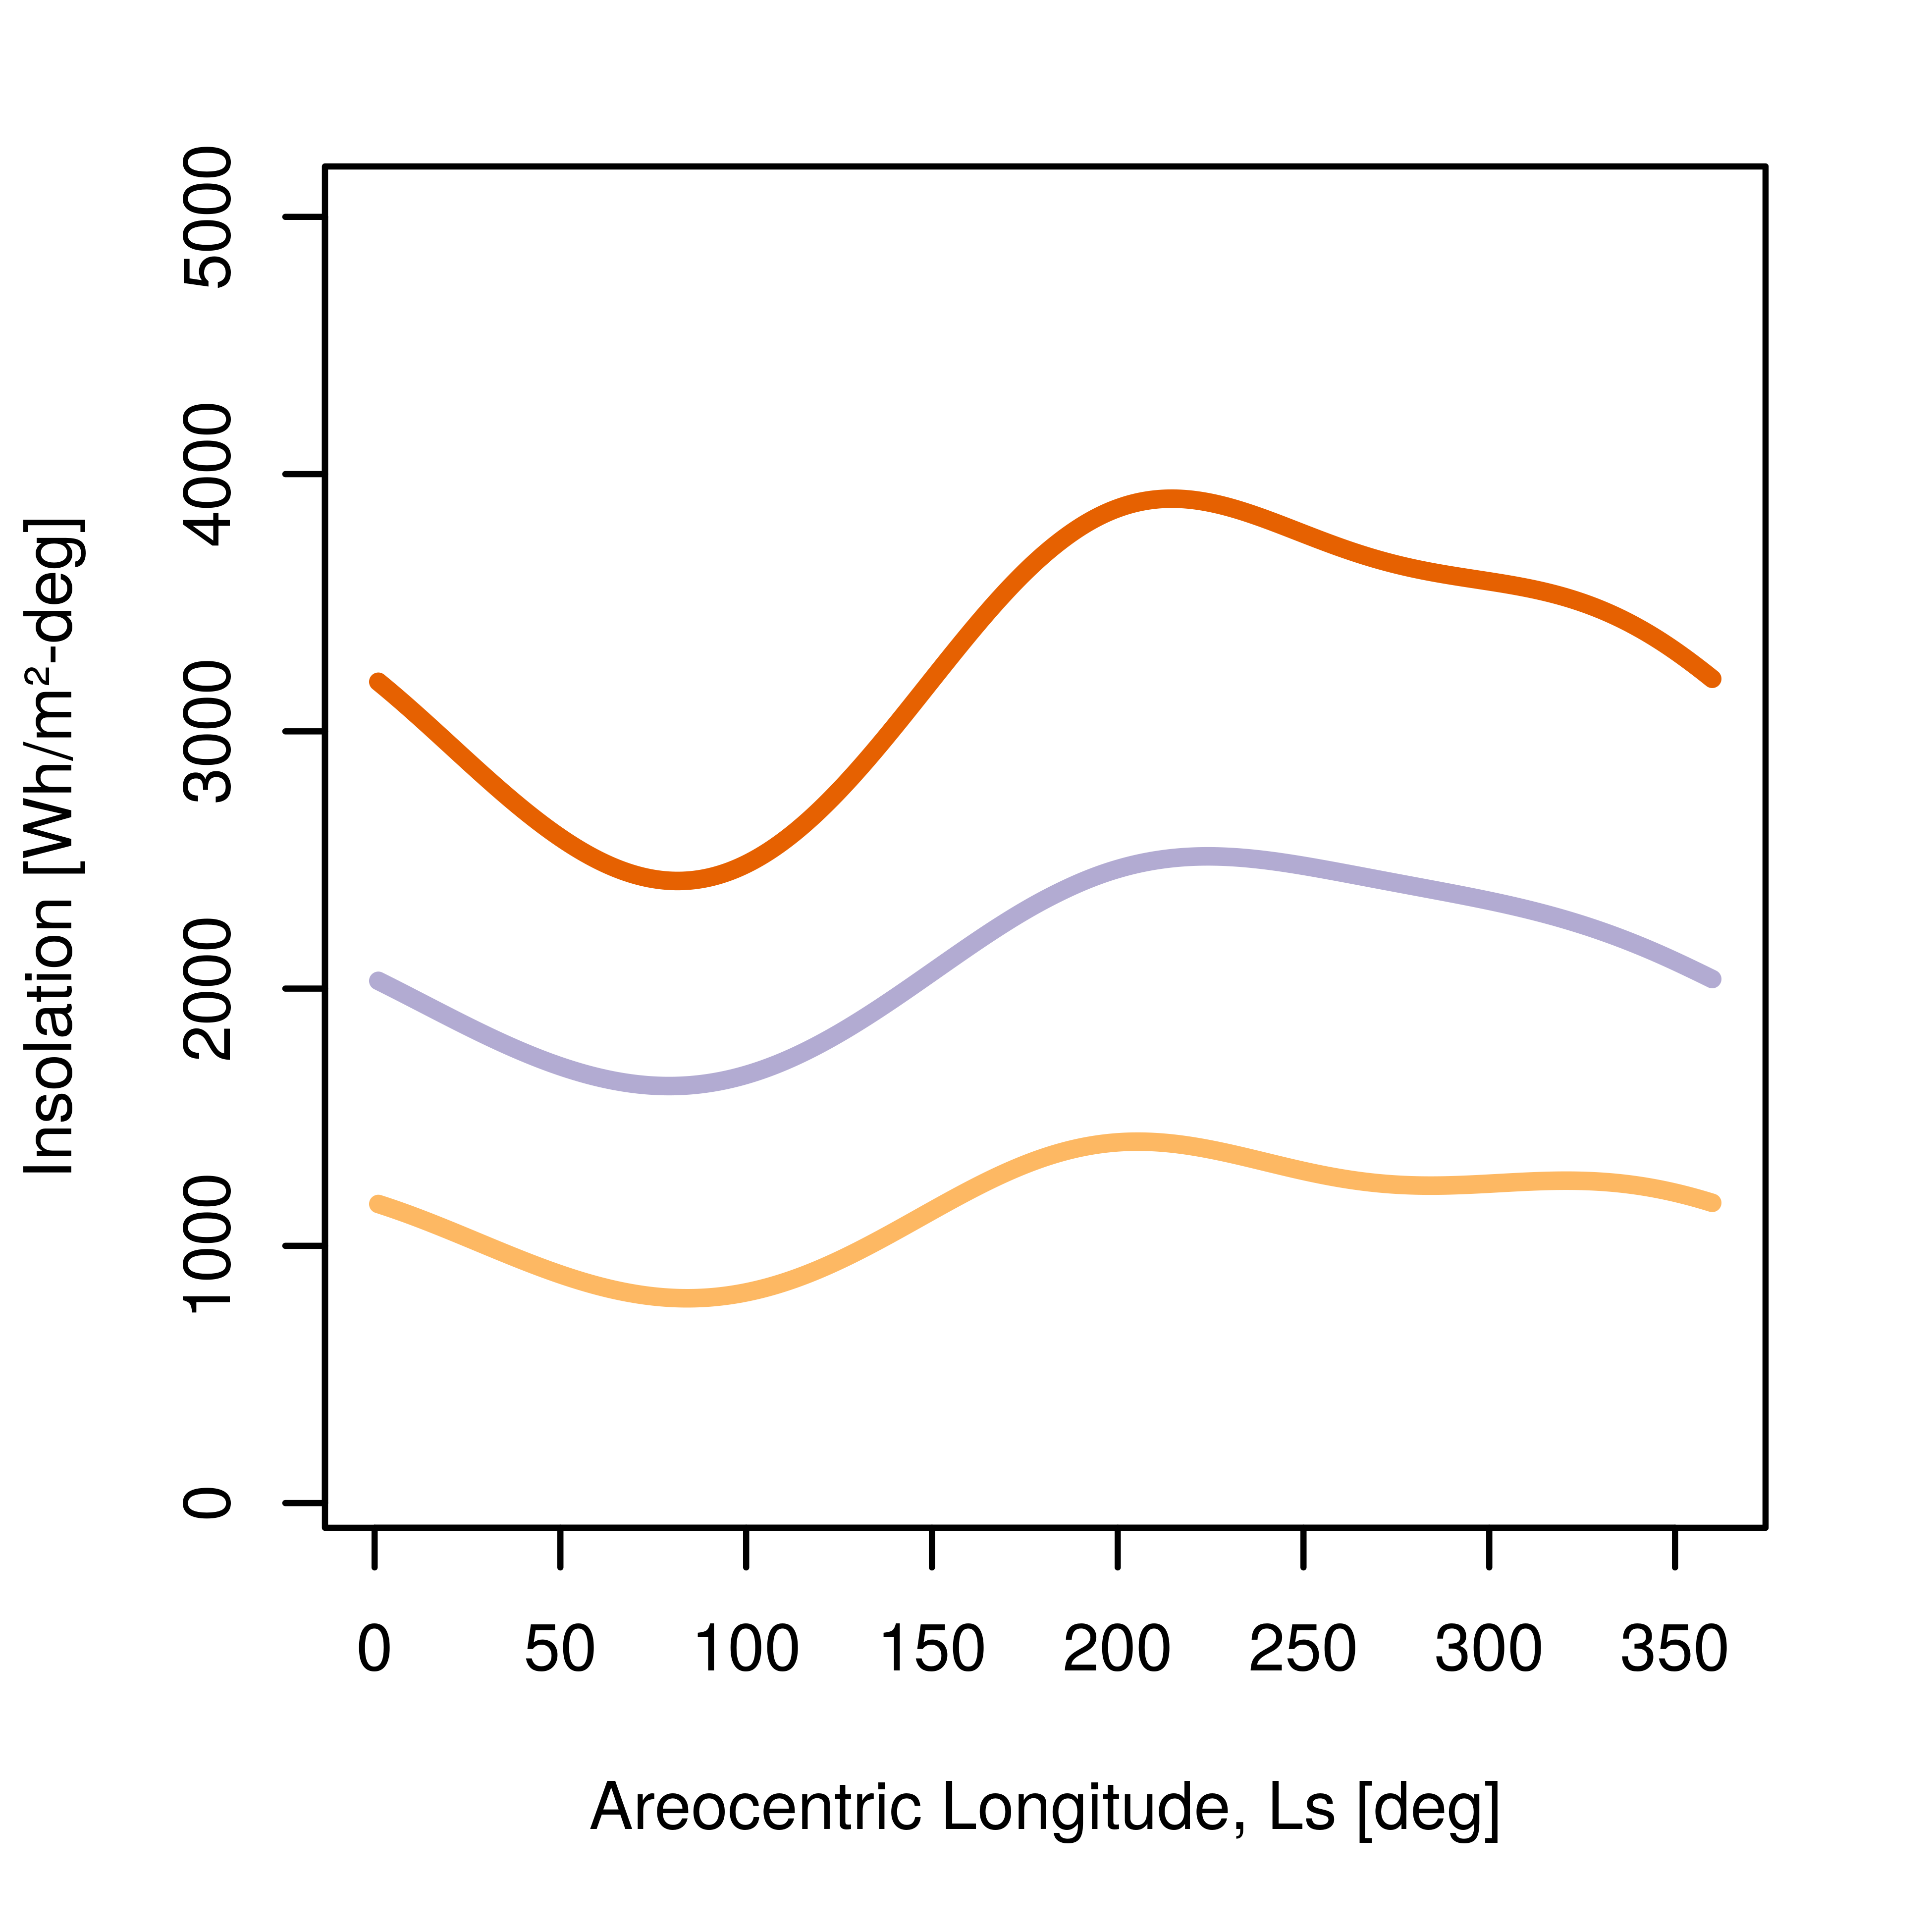
\includegraphics[height=\graphicsHeight]{sections/mars-solar-energy/solar-radiation/plots/hh-hbh-and-hdh-as-a-function-of-ls-for-tau1-phi205-and-albedo-027}
  		\subcaption{$\tau = 1$}
  		\label{fig:sub:insolation-ls-tau-factor-1}
  	\end{subfigure}\\[0.8ex]
%% 2nd row
    \begin{subfigure}[t]{\subfigureWidth}
      \centering
  		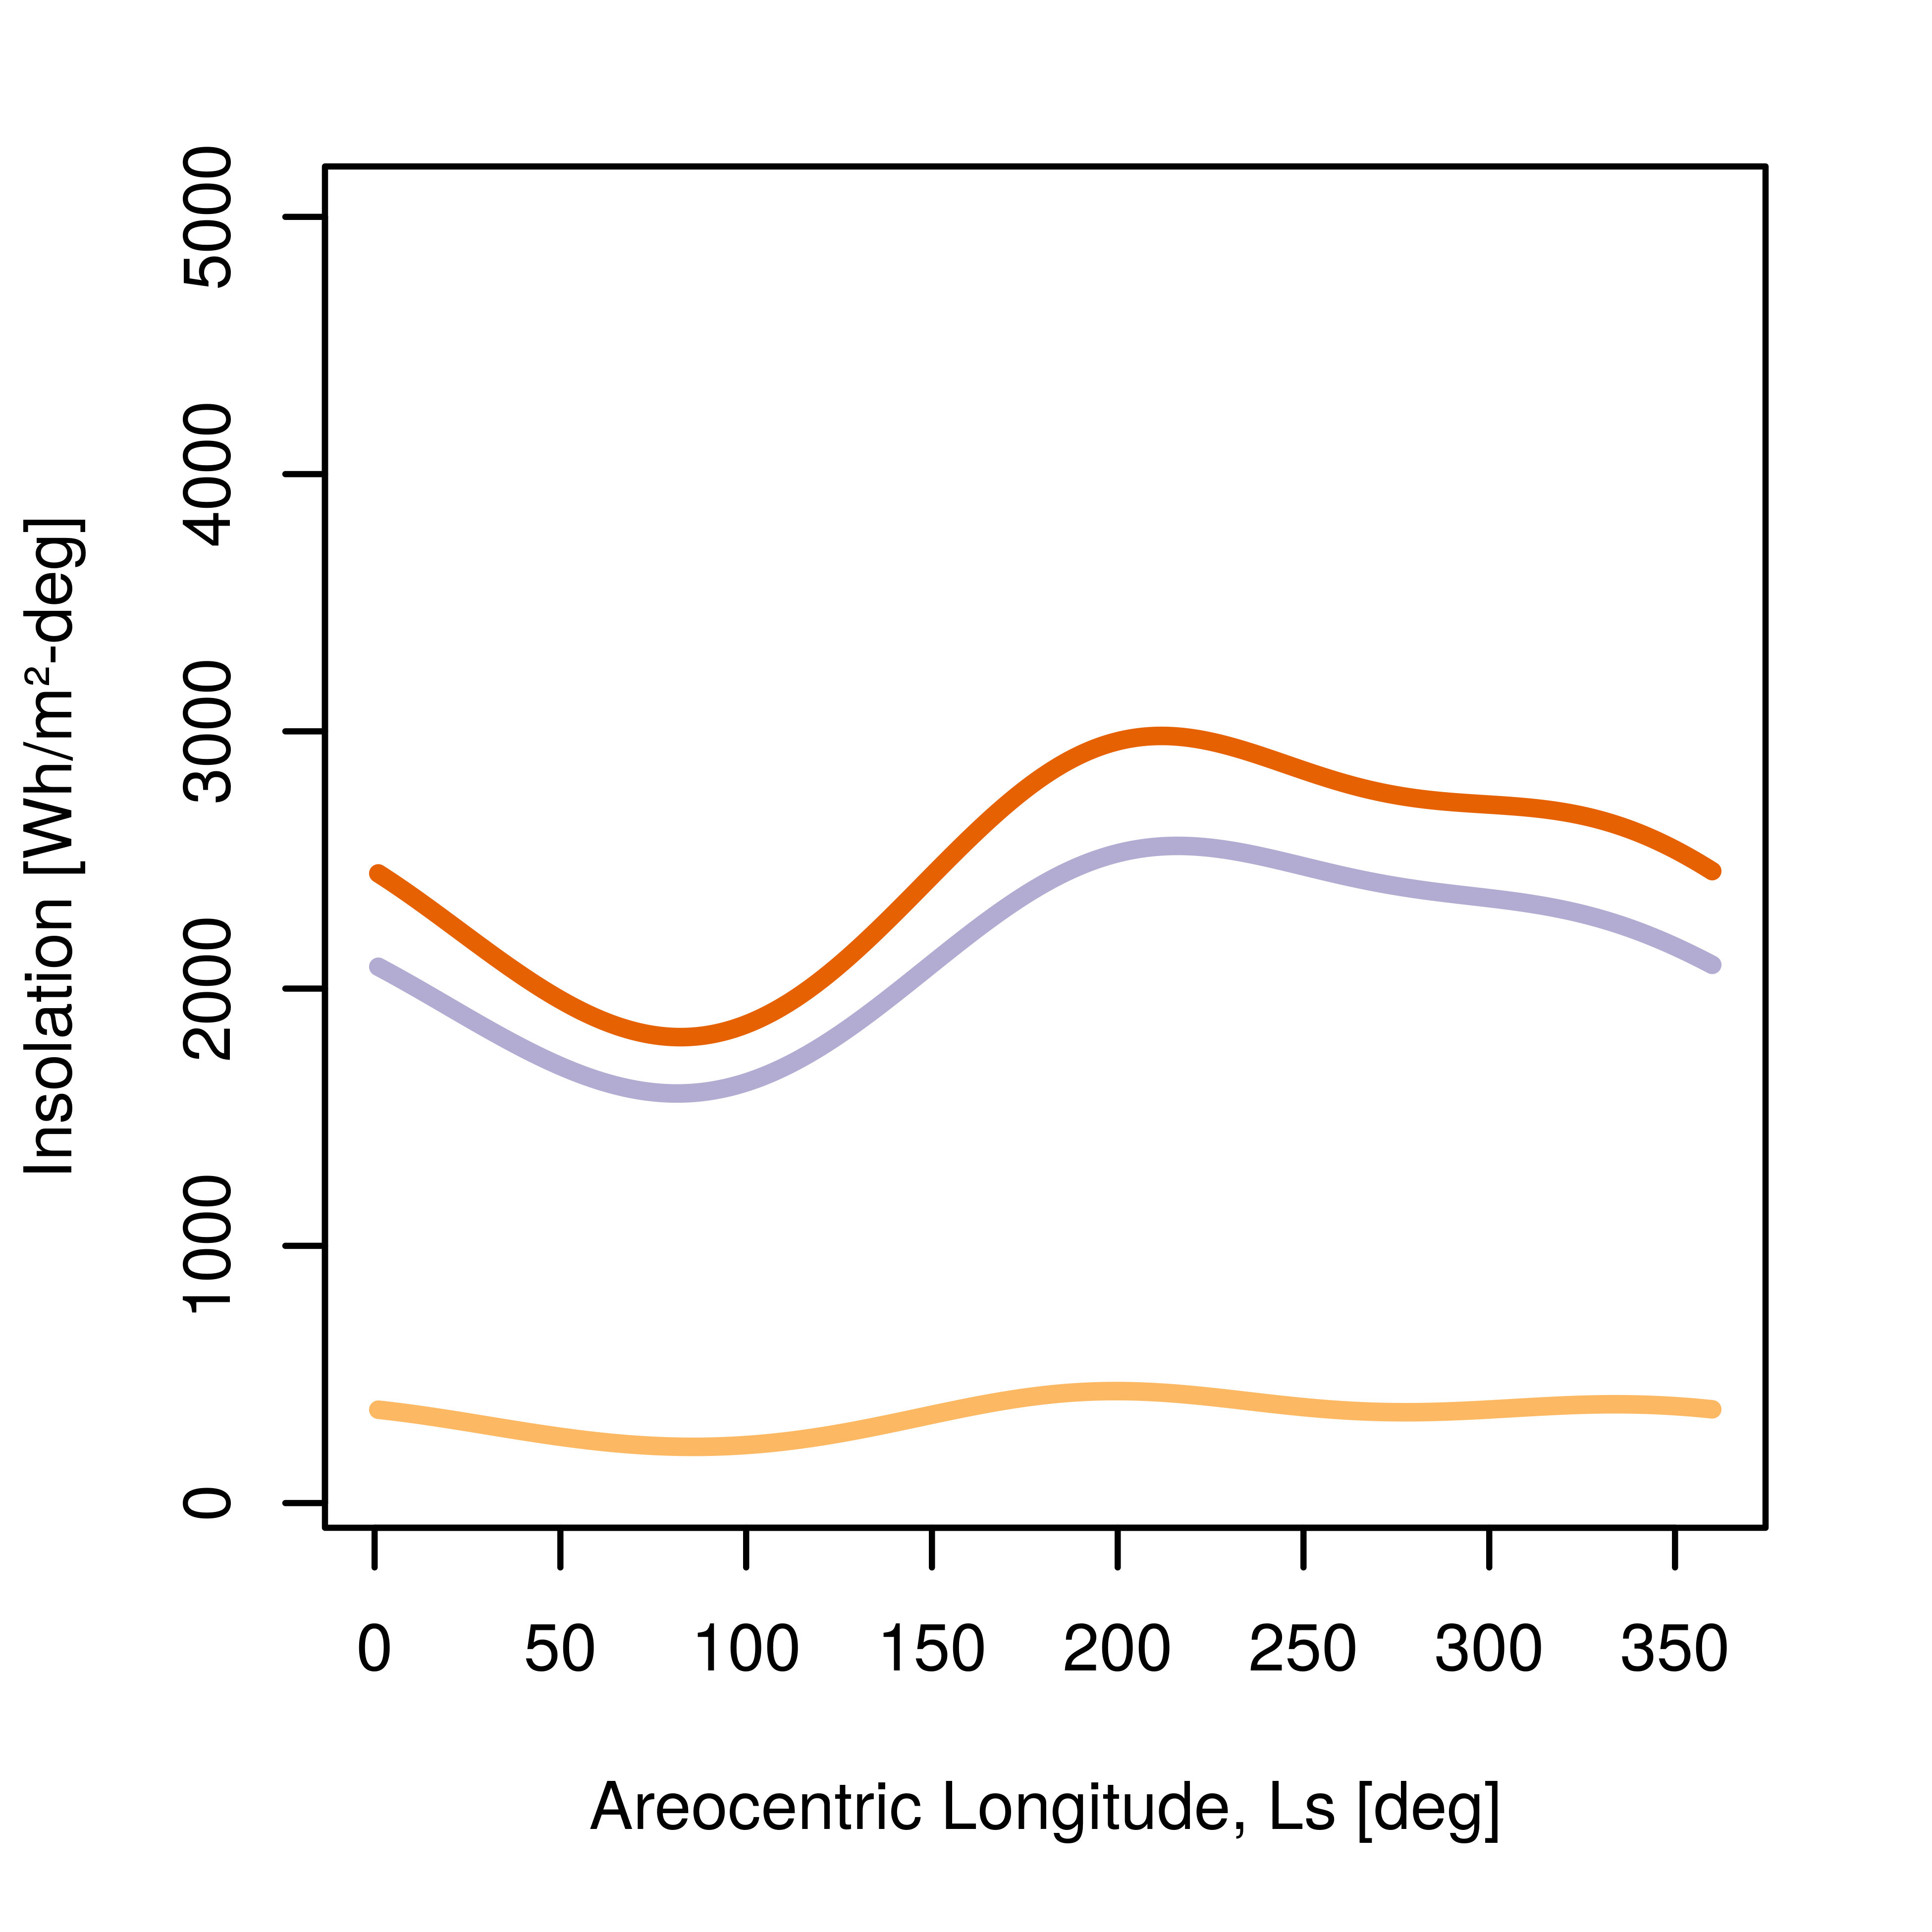
\includegraphics[height=\graphicsHeight]{sections/mars-solar-energy/solar-radiation/plots/hh-hbh-and-hdh-as-a-function-of-ls-for-tau2-phi205-and-albedo-027}
  		\subcaption{$\tau = 2$}
  		\label{fig:sub:insolation-ls-tau-factor-2}
  	\end{subfigure}\hfill
	   \begin{subfigure}[t]{\subfigureWidth}
      \centering
  		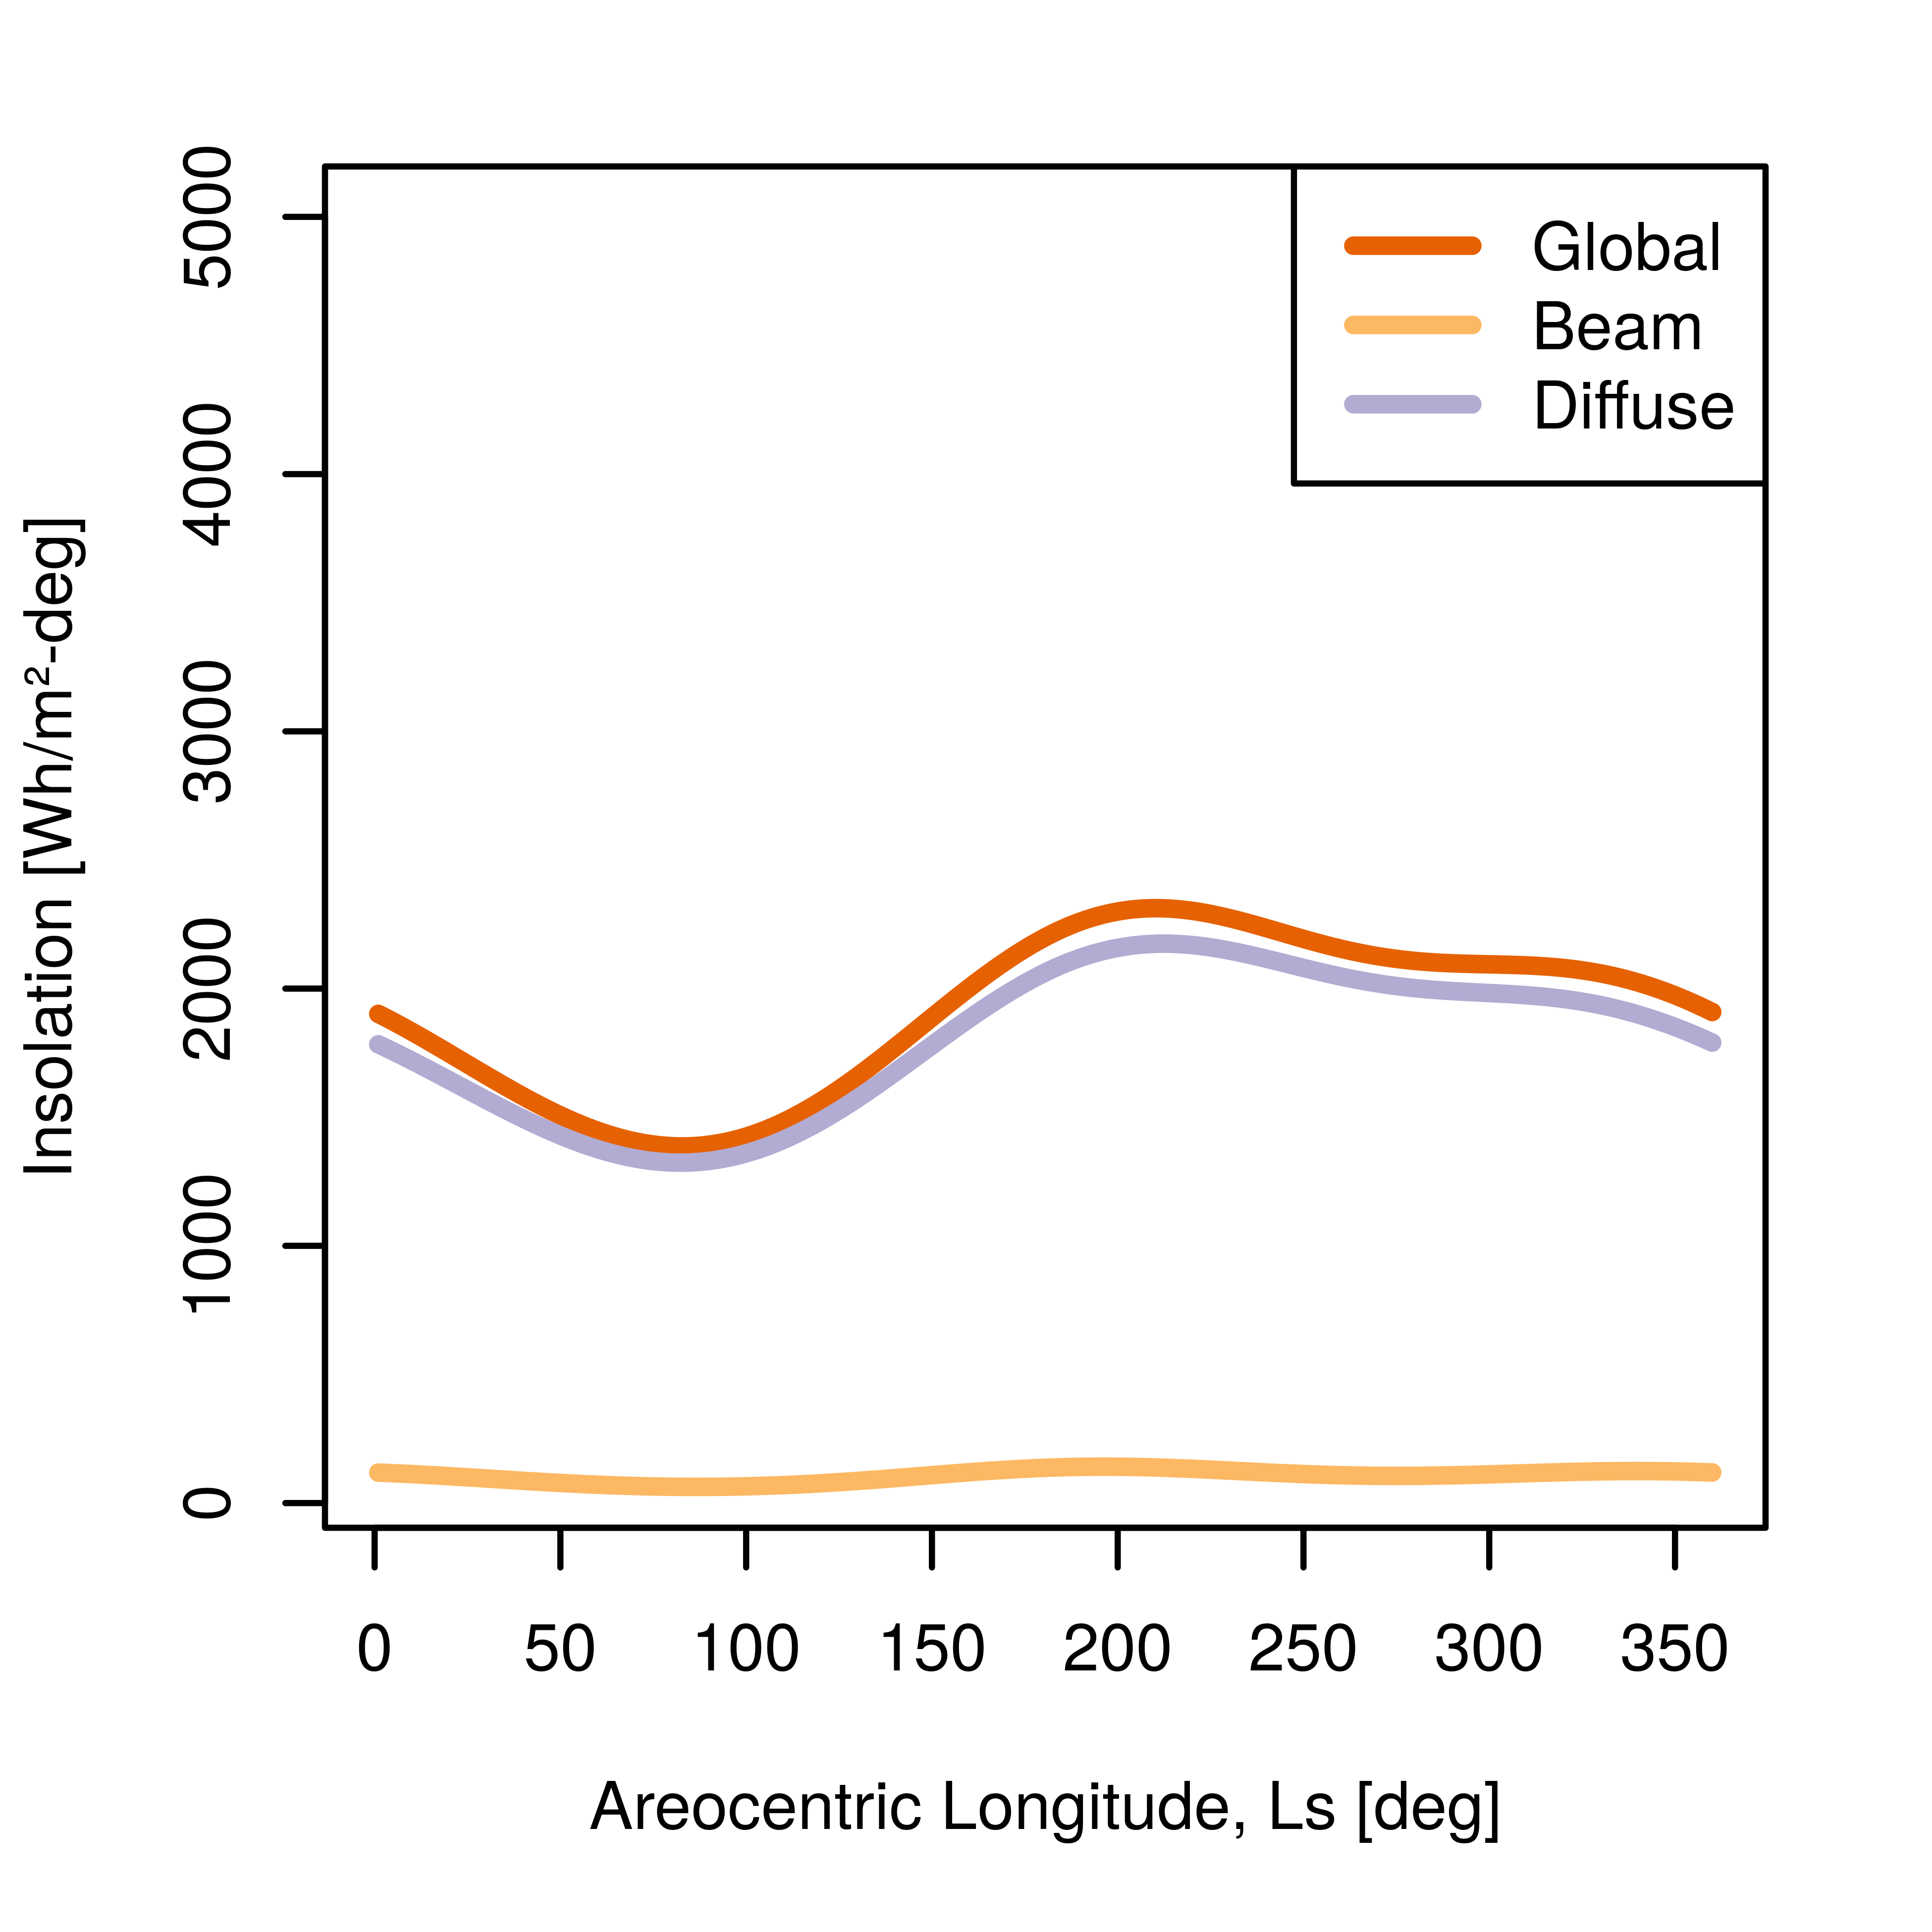
\includegraphics[height=\graphicsHeight]{sections/mars-solar-energy/solar-radiation/plots/hh-hbh-and-hdh-as-a-function-of-ls-for-tau3-phi205-and-albedo-027}
  		\subcaption{$\tau = 3$}
  		\label{fig:sub:insolation-ls-tau-factor-3}
	   \end{subfigure}\hfill
	\caption{Variation of global, beam, and diffuse insolation on Mars horizontal surface as a function of areocentric longitude at Endeavour Crater.}
	\label{fig:plot:insolation-ls}
\vspace{-2ex}
\end{figure}

Daily insolations are obtained when $\omega_1$ and $\omega_2$ are set for a time period between sunrise and sunset. These insolations are denoted as $H_{h}$, $H_{bh}$, and $H_{dh}$ for global, beam, and diffuse insolations on Mars horizontal surface and $H_{obh}$ for a horizontal surface at the top of Mars atmosphere. Similarly to $I_{dh}$, the daily diffuse insolations $H_{dh}$ is obtained from the same relationship presented in Equation \ref{eq:G_h_1}.

To illustrate the variation of beam, direct, and diffuse insolations during a Martian day, a diurnal profile is presented in Figure \ref{fig:plot:insolation-phi} at different planetary latitudes during the aphelion for a clear day with $\tau = 0.5$. The seasonal influences are evident: at $L_{s} = \SI{71}{\degree}$, it is Autumn in the northern hemisphere and insolations at $\phi = \SI{20}{\degree}$ are much greater than those in the southern hemisphere at $\phi = \SI{-20}{\degree}$ and $\phi = \SI{-40}{\degree}$. Furthermore, daylight at $\phi = \SI{20}{\degree}$ spans across 16 hours whereas they only last for 12 hours at $\phi = \SI{-20}{\degree}$ and 10 hours at $\phi = \SI{-40}{\degree}$ .


\begin{figure}[h]
\captionsetup[subfigure]{justification=centering}
\vspace{-2ex}
	\centering
    %% setup sizes
    \setlength{\subfigureWidth}{0.50\textwidth}
    \setlength{\graphicsHeight}{80mm}
    %% kill hyper-link highlighting
    \hypersetup{hidelinks=true}%
    %% the figures
%% 1st row
  	\begin{subfigure}[t]{\subfigureWidth}
      \centering
  		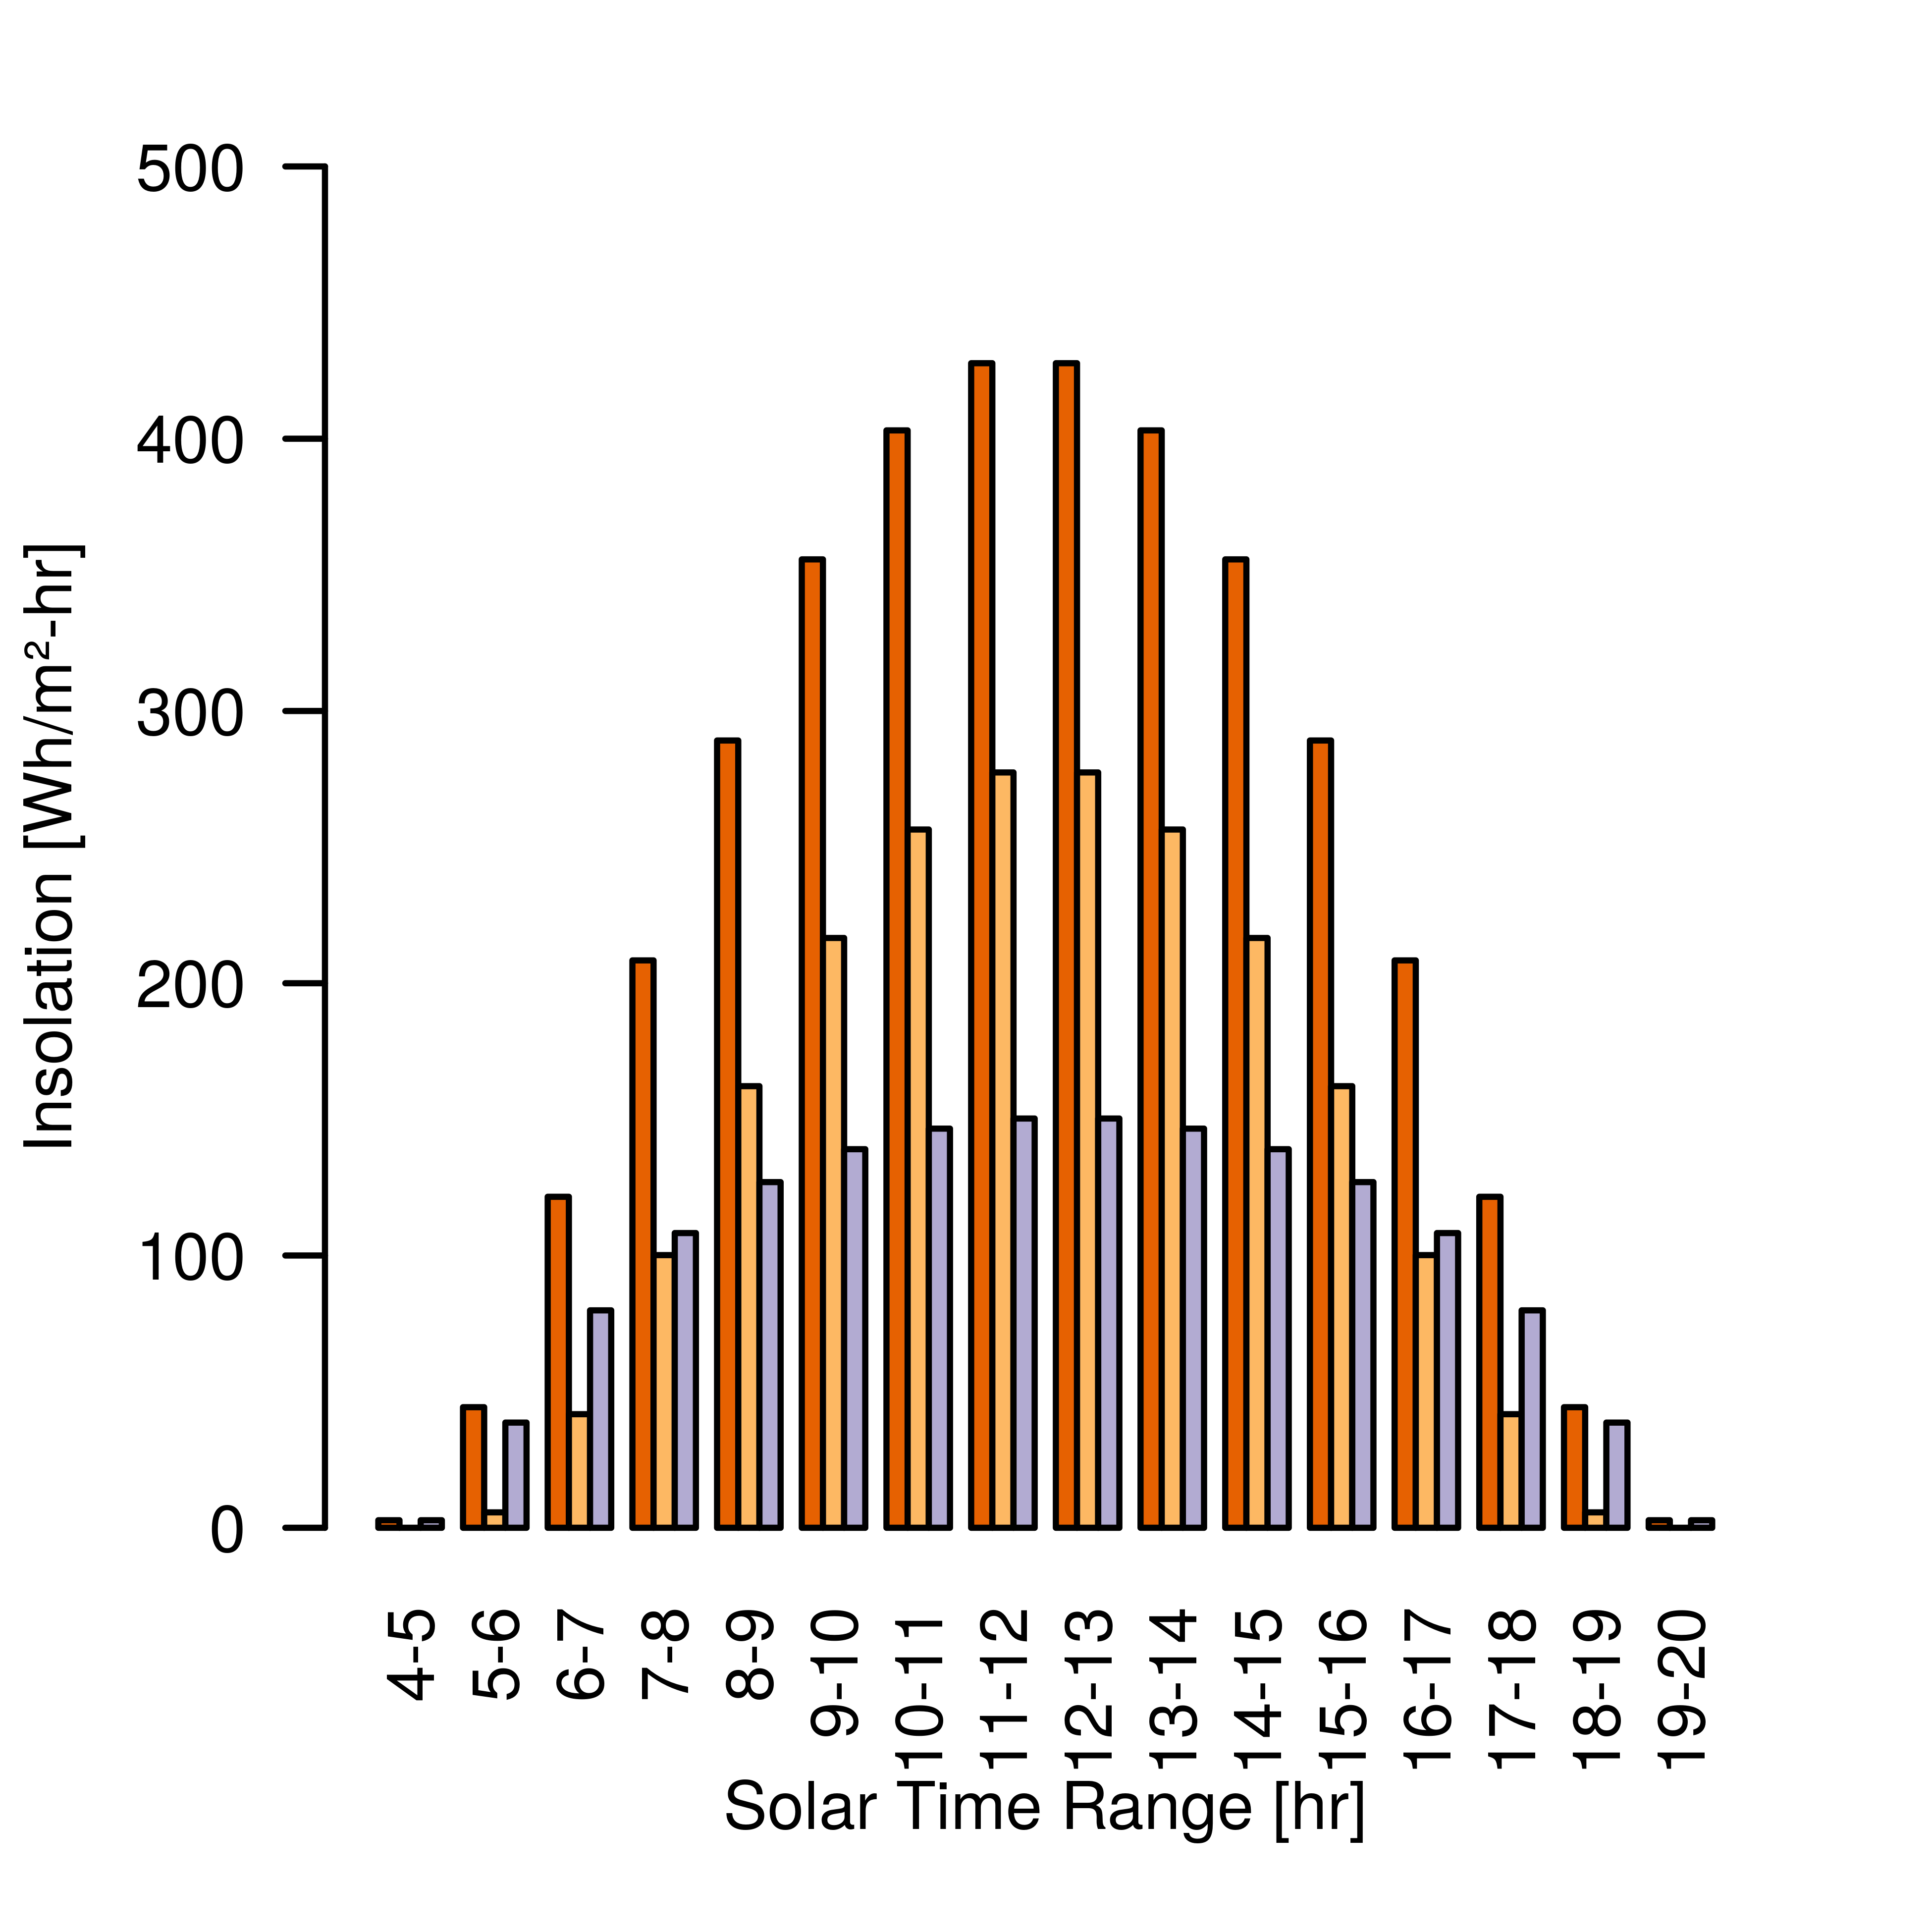
\includegraphics[height=\graphicsHeight]{sections/mars-solar-energy/solar-radiation/plots/ih-ibh-and-idh-variation-1-for-ls-71-phi-40-tau-05-and-albedo-027}
  		\subcaption{$\phi = \SI{40}{\degree}$}
  		\label{fig:sub:insolation-phi-m40}
  	\end{subfigure}\hfill
    \begin{subfigure}[t]{\subfigureWidth}
      \centering
  		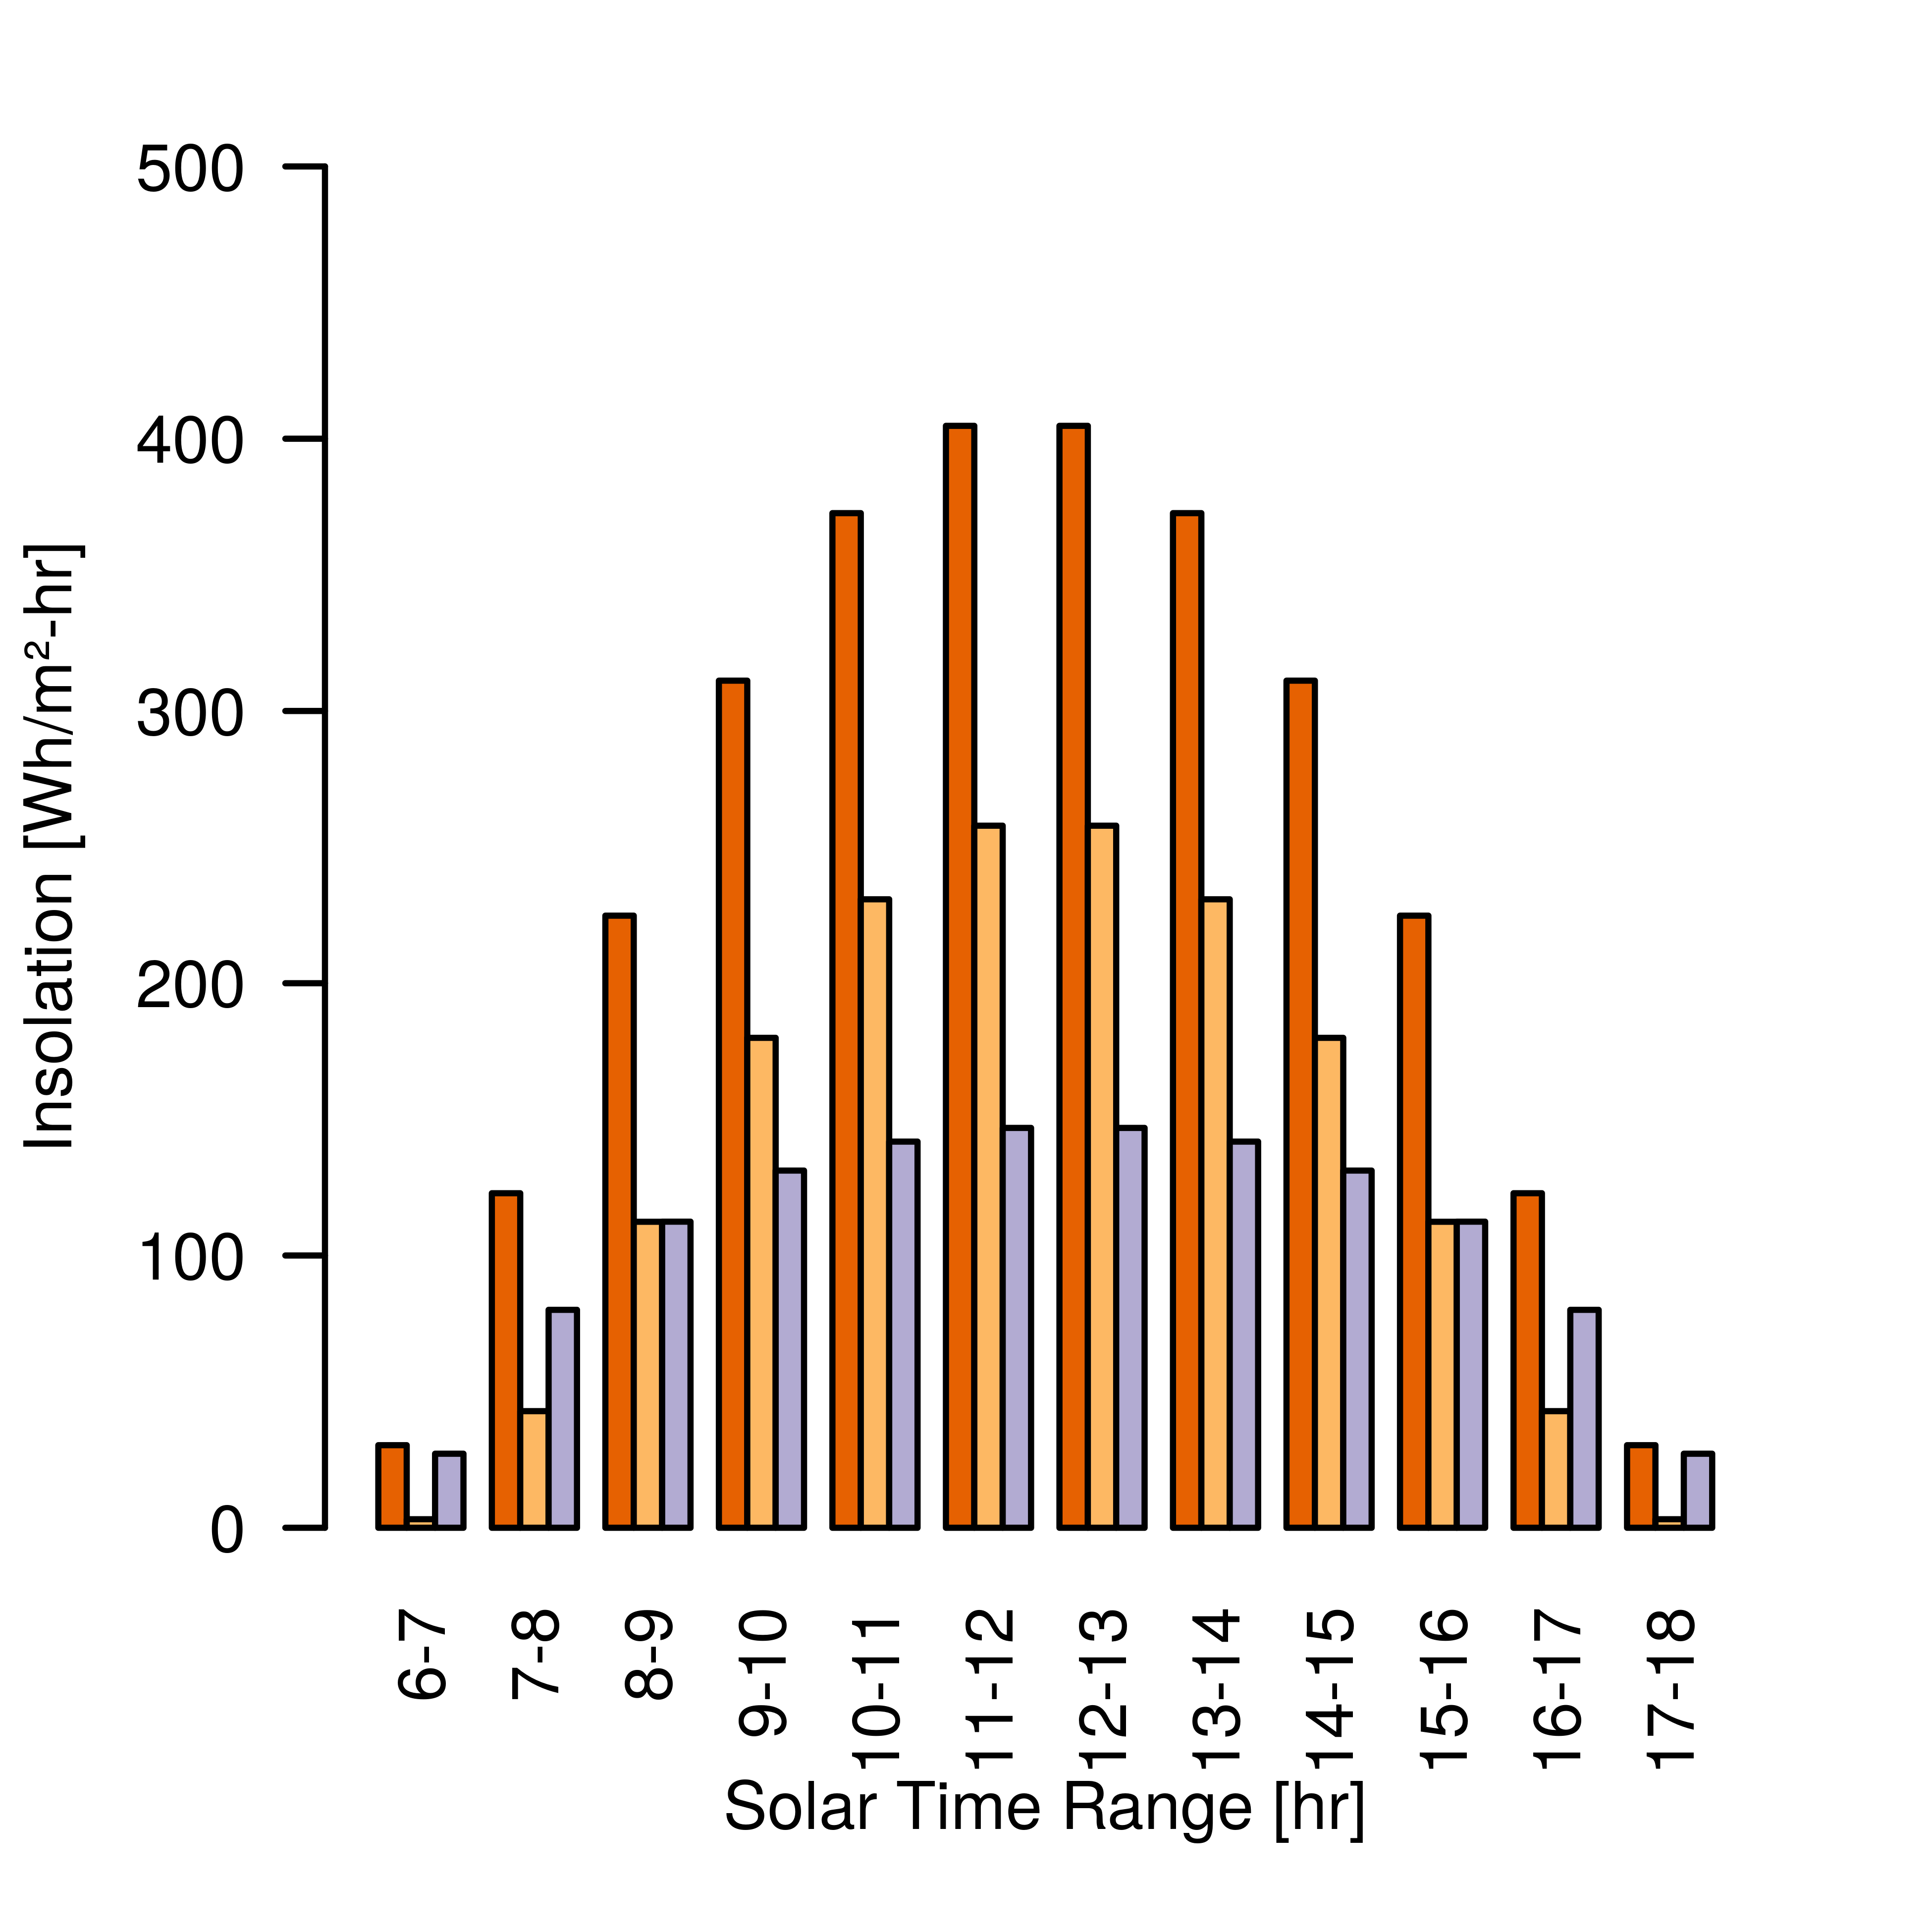
\includegraphics[height=\graphicsHeight]{sections/mars-solar-energy/solar-radiation/plots/ih-ibh-and-idh-variation-2-for-ls-71-phi-0-tau-05-and-albedo-027}
  		\subcaption{$\phi = \SI{0}{\degree}$}
  		\label{fig:sub:insolation-phi-m20}
  	\end{subfigure}\\[0.8ex]
%% 2nd row
    \begin{subfigure}[t]{\subfigureWidth}
      \centering
  		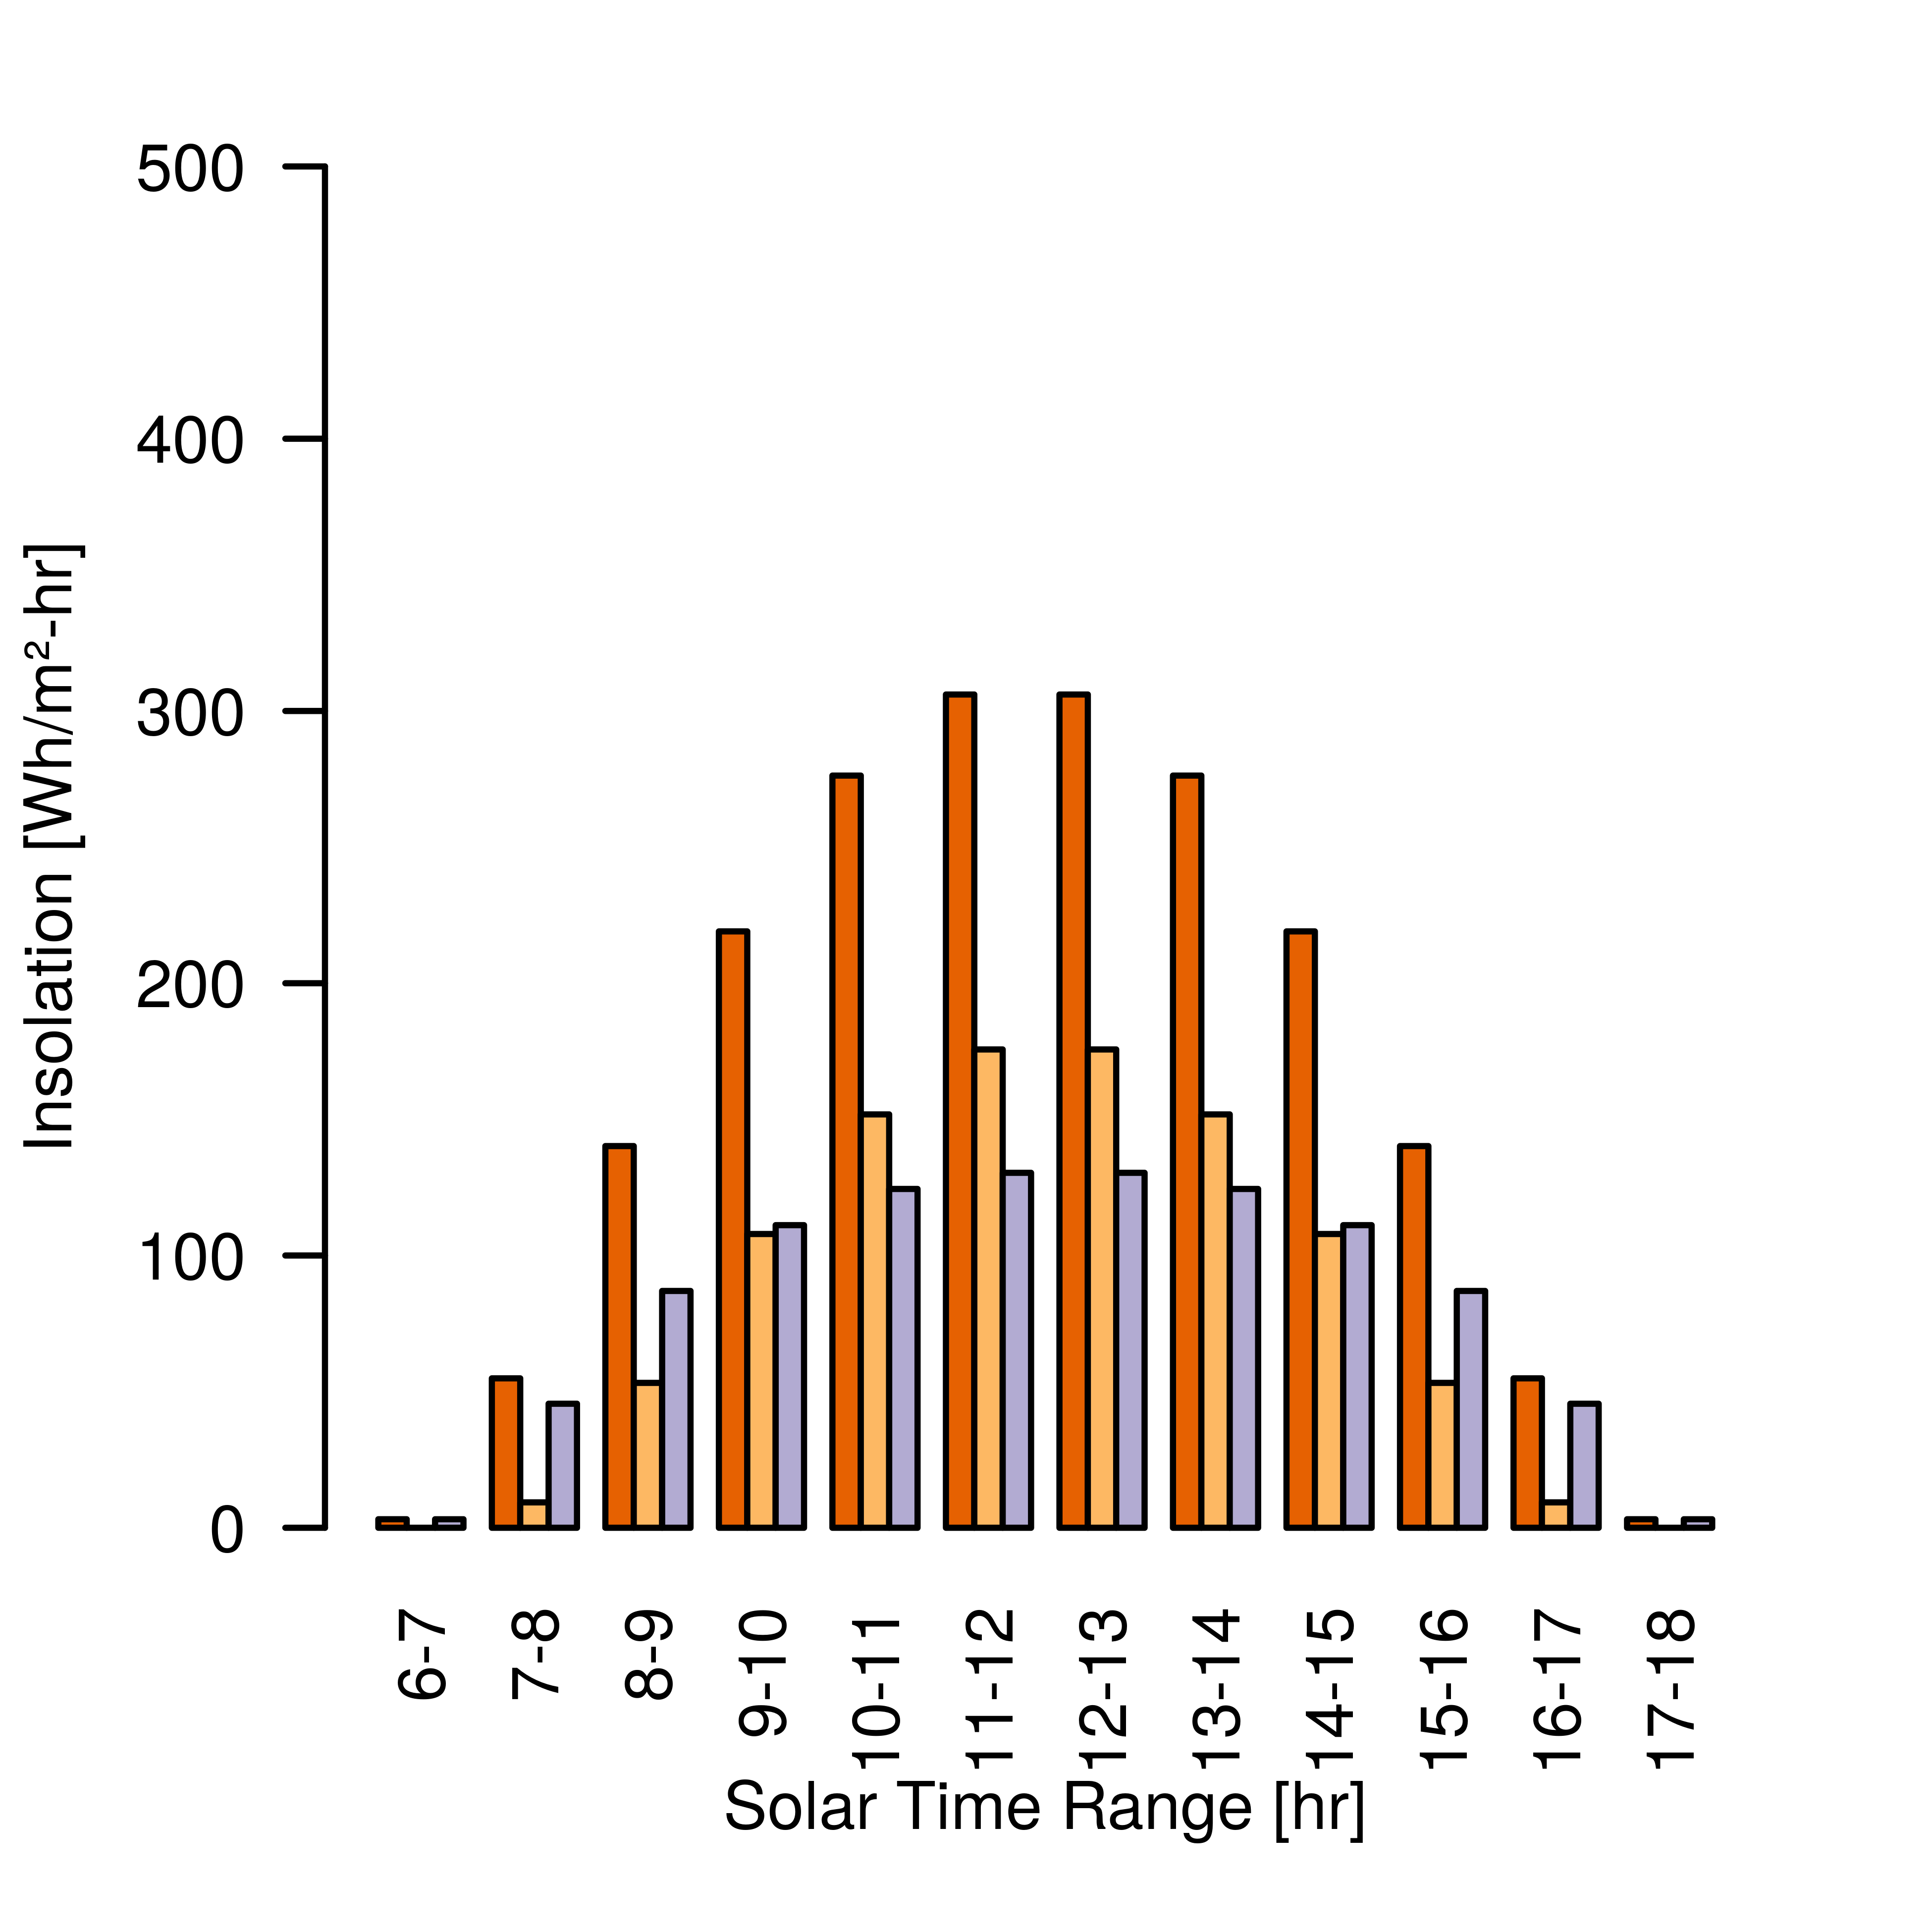
\includegraphics[height=\graphicsHeight]{sections/mars-solar-energy/solar-radiation/plots/ih-ibh-and-idh-variation-3-for-ls-71-phi-20-tau-05-and-albedo-027}
  		\subcaption{$\phi = \SI{-20}{\degree}$}
  		\label{fig:sub:insolation-phi-0}
  	\end{subfigure}\hfill
	   \begin{subfigure}[t]{\subfigureWidth}
      \centering
  		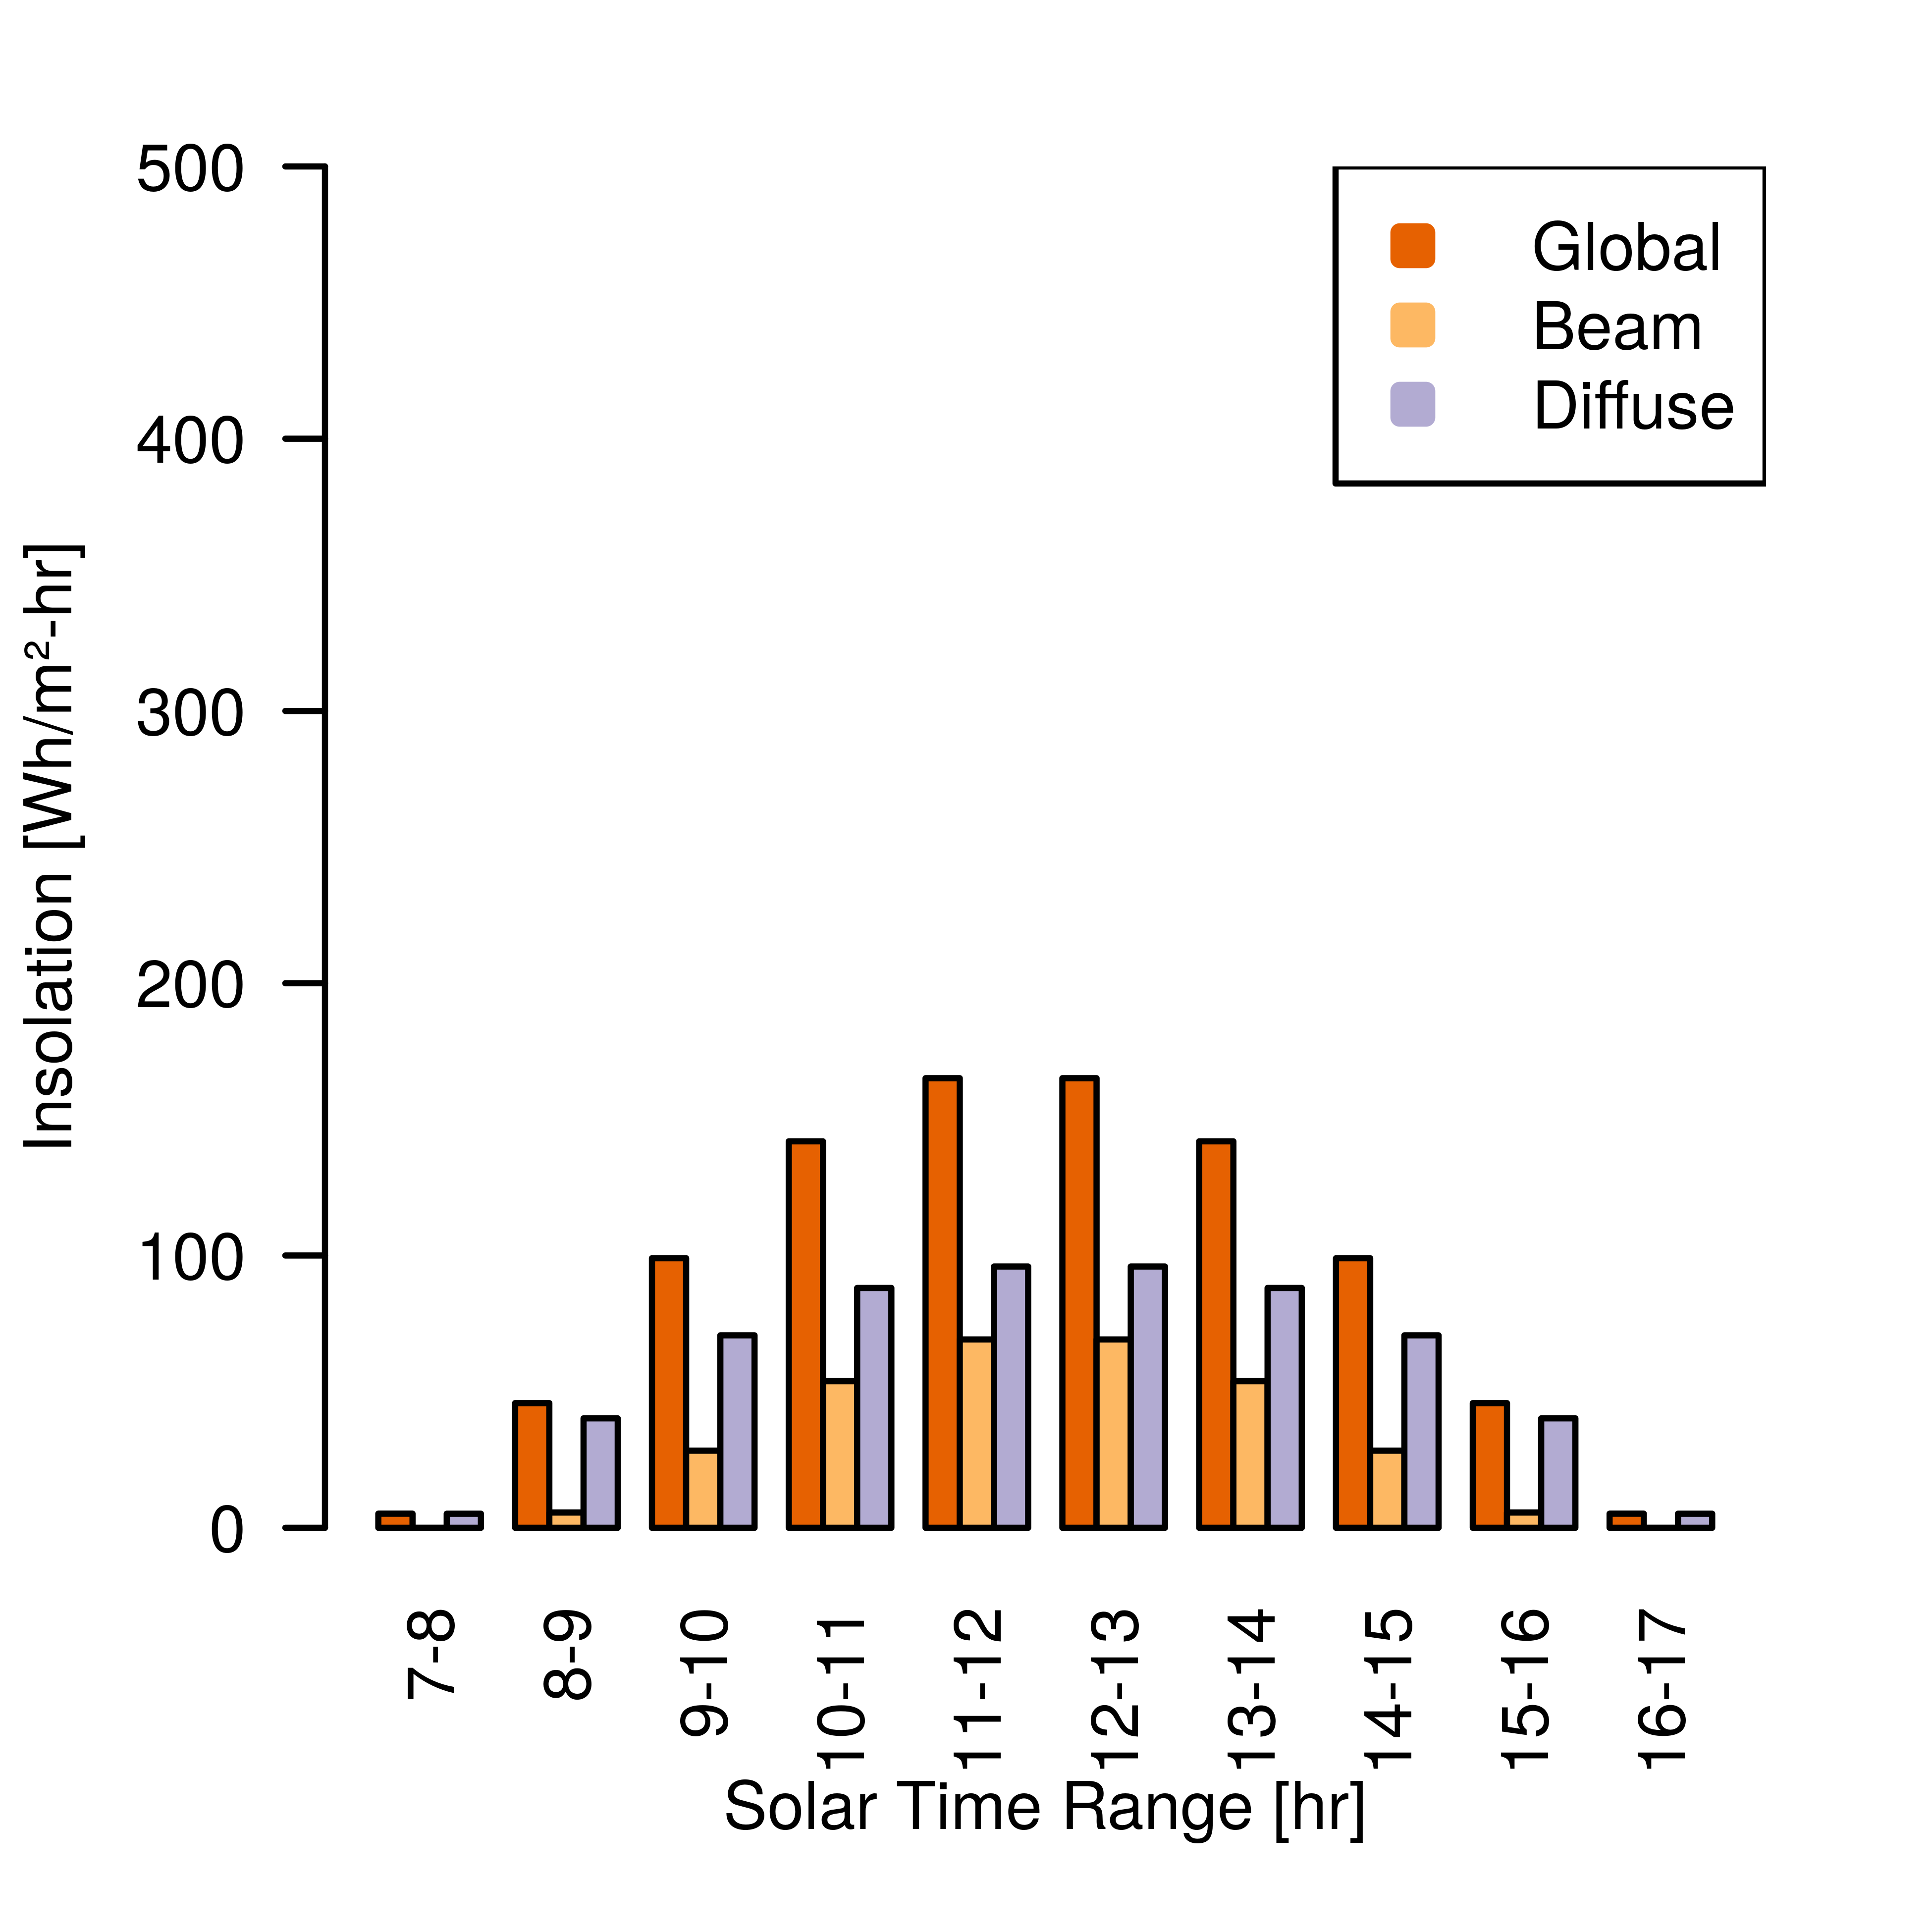
\includegraphics[height=\graphicsHeight]{sections/mars-solar-energy/solar-radiation/plots/ih-ibh-and-idh-variation-4-for-ls-71-phi-40-tau-05-and-albedo-027}
  		\subcaption{$\phi = \SI{-40}{\degree}$}
  		\label{fig:sub:insolation-phi-p20}
	   \end{subfigure}\hfill
	\caption{Diurnal variation of global, beam, and diffuse insolation on Mars horizontal surface at different planetary latitudes.}
	\label{fig:plot:insolation-phi}
\vspace{-2ex}
\end{figure}

\clearpage
\subsubsection{Inclined Surface}
\label{sec:MartianEnvironment:SolarRadiation:InclinedSurface}

Hitherto the irradiance and insolation calculations on the surface of Mars have been restricted to a horizontal plane. Inclined surfaces were also considered so that \ac{SA} energy production may be maximized during the following cases:
\begin{itemize}
    \item Taking advantage of the active suspension system to tilt and orient the \ac{SA} surface into optimal angles while the rover is on a horizontal surface.
    \item Taking advantage of the active suspension system to tilt and orient the \ac{SA} into a horizontal plane while the rover is on an inclined surface.
    \item Traversing descent and ascent profiles such as with the topographic slope variation in crater exploration missions.
\end{itemize}

Descriptions of the angles involved as well as how they serve to position the \ac{SA} surface are presented in Appendix \ref{sec:Appendix:OptimalAngles}. Global irradiance $G_{\beta}$ on an inclined surface can be obtained when parametizing the inclination angle $\beta$ and the Sun angle of incidence $\theta$:

\begin{equation}
  \label{eq:G_beta}
  G_{\beta} = G_{b}\cos{\theta} + G_{dh}\cos{\left(\frac{\beta}{2}\right)}^2 + al G_{h} \sin{\left(\frac{\beta}{2}\right)}^2
\end{equation}

where $al$ is the albedo.

The Sun angle of incidence itself is a function of the Sun zenith angle $z$ for the time of day, the slope angle $\beta$ for the inclination, and the solar azimuth $\gamma_{s}$ as well as the Sun surface azimuth angle $\gamma_{c}$ for the orientation that the inclination is facing:

\begin{equation}
  \label{eq:costheta}
  \cos{\theta} = \cos{\beta}\cos{z} +  \sin{\beta}\sin{z}\cos{(\gamma_{s} - \gamma_{c})}
\end{equation}

where the Sun zenith angle is given by Equation \ref{eq:cosz}.

Variation of the global irradiance at the perihelion for different inclination angles are presented in Figure \ref{fig:plot:irradiance-inclined-gamma-c} for South, East, North, and West slope orientations. The influence of the inclination angle is most noticeable for a \SI{20}{\degree} slope oriented southwards resulting in a stronger irradiance profile than all other showcased slope angle and orientation configurations.

\begin{figure}[h]
\captionsetup[subfigure]{justification=centering}
\vspace{-2ex}
	\centering
    %% setup sizes
    \setlength{\subfigureWidth}{0.50\textwidth}
    \setlength{\graphicsHeight}{80mm}
    %% kill hyper-link highlighting
    \hypersetup{hidelinks=true}%
    %% the figures
%% 1st row
  	\begin{subfigure}[t]{\subfigureWidth}
      \centering
  		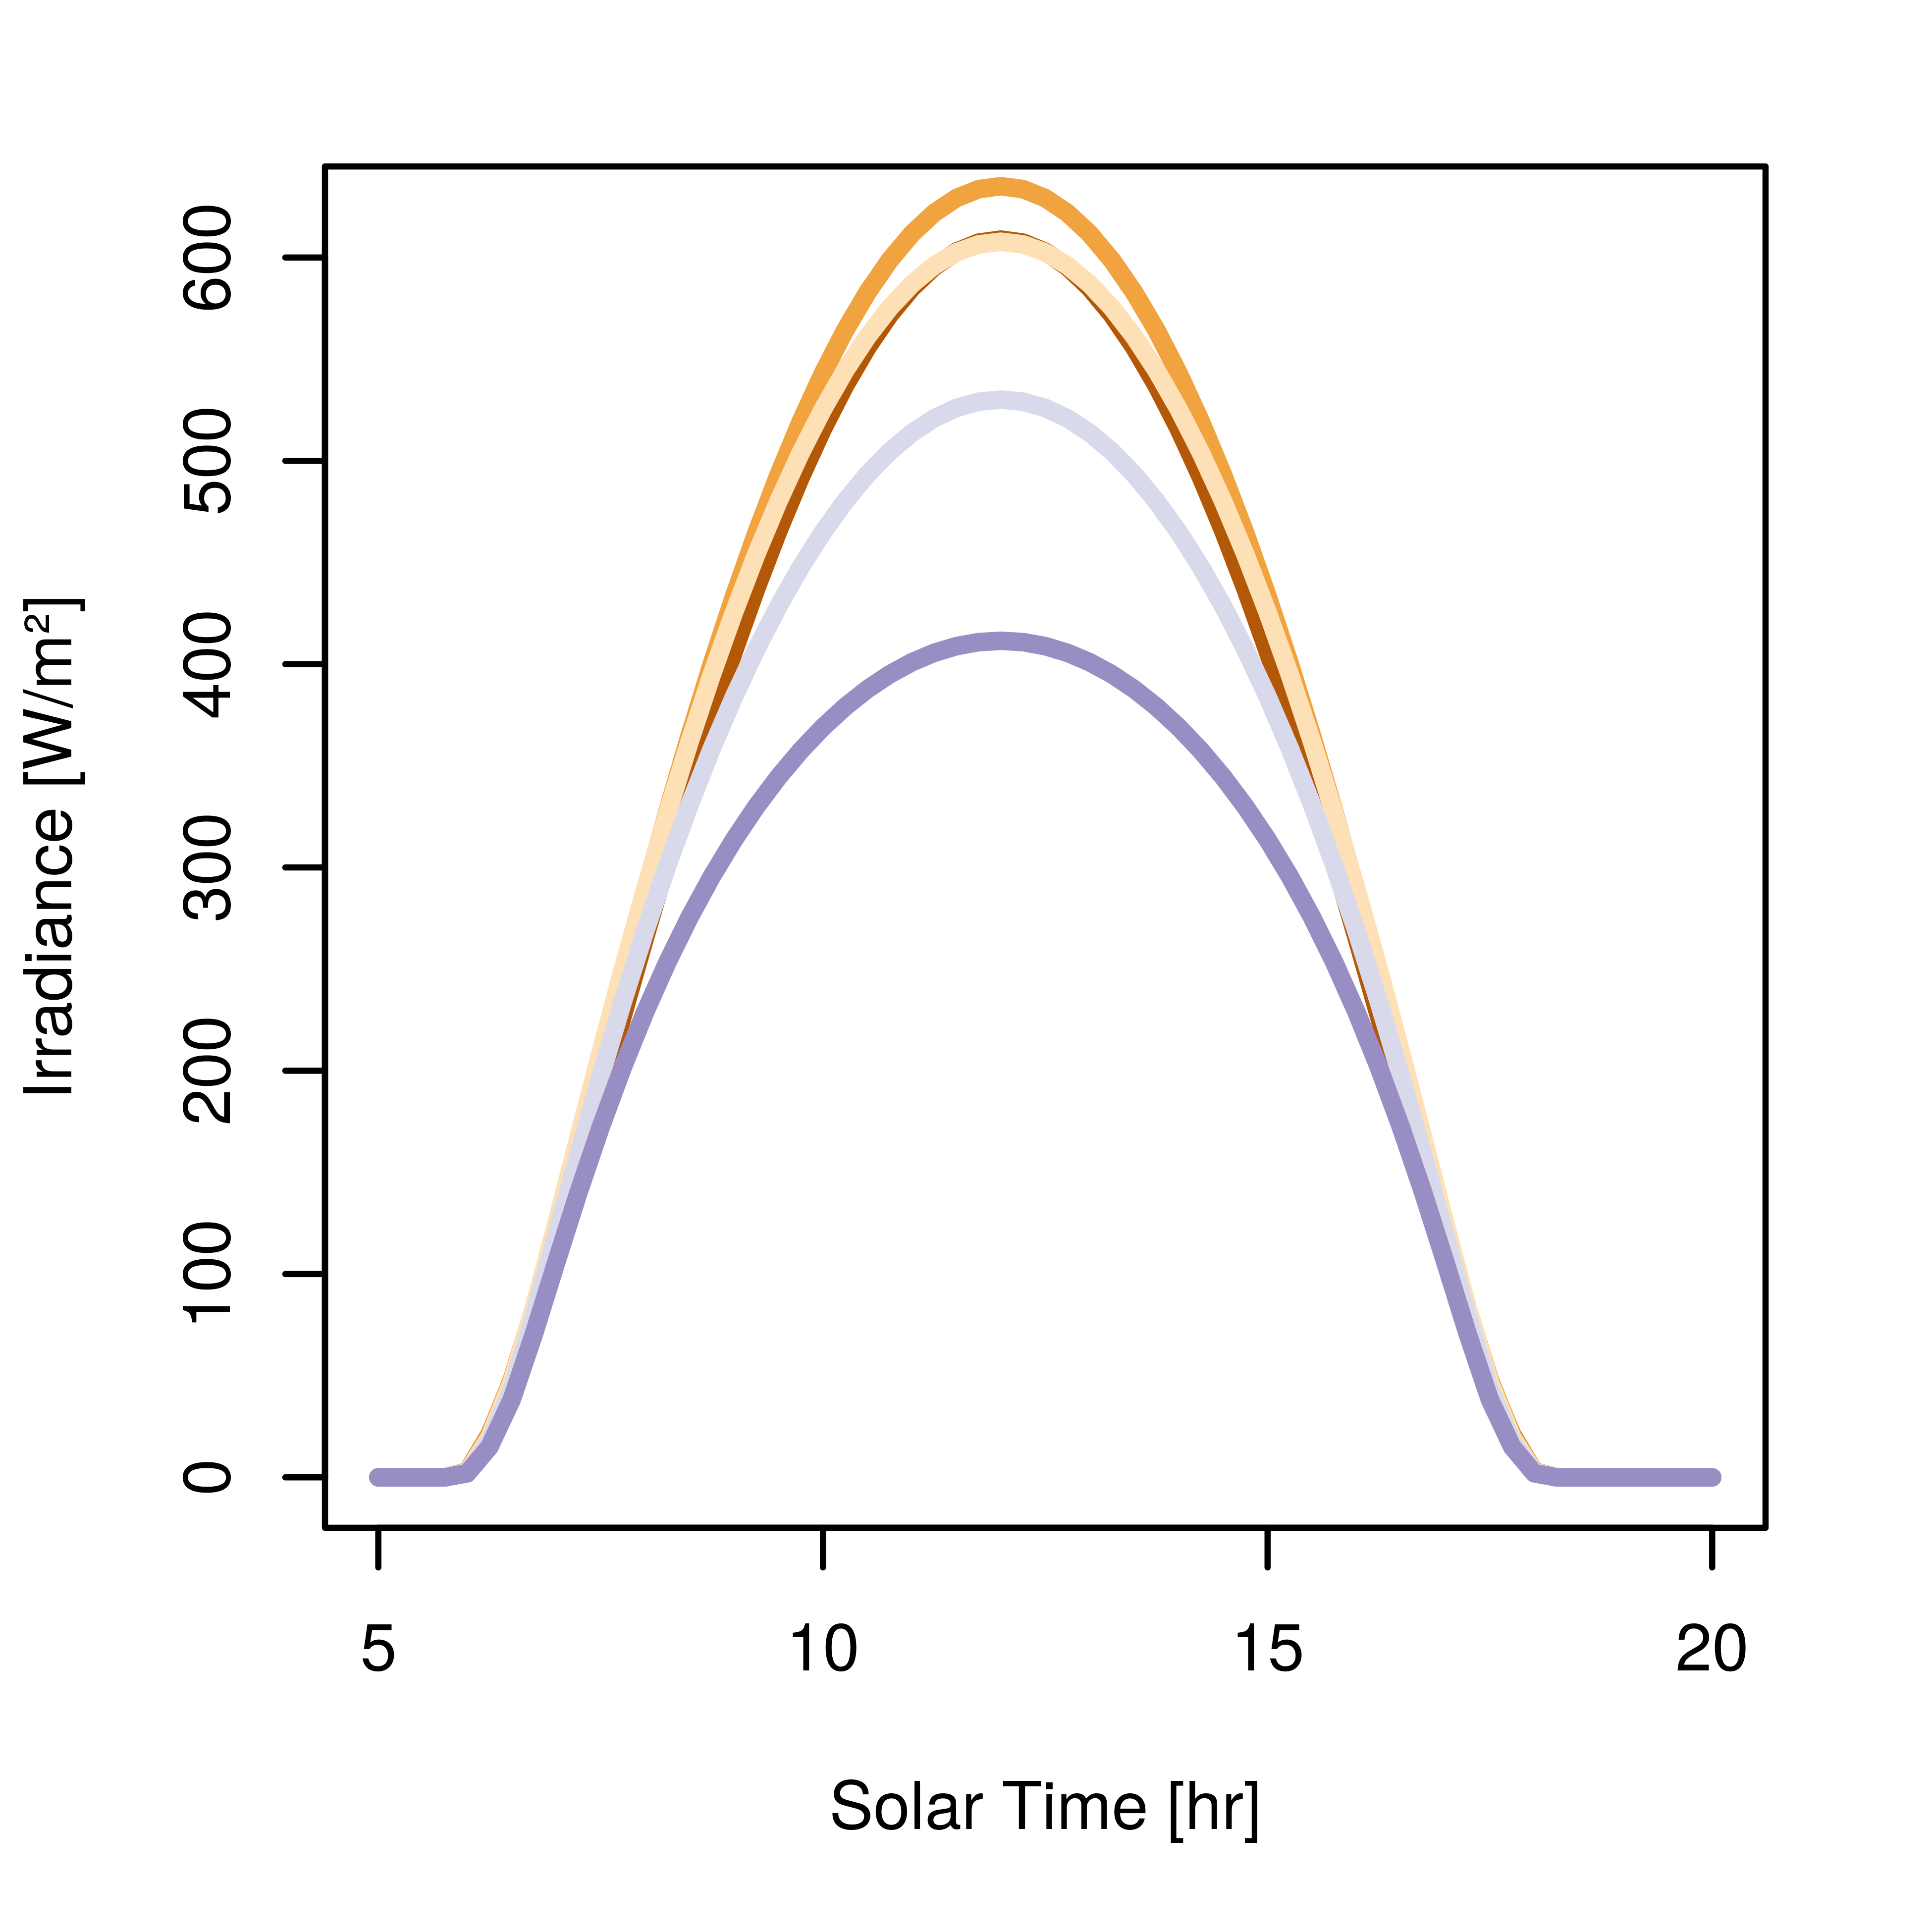
\includegraphics[height=\graphicsHeight]{sections/mars-solar-energy/solar-radiation/plots/gi-variationfor-ls-248-phi-2-tau-05-gammac-north-and-albedo-027.png}
  		\subcaption{$\gamma_{c} = \SI{0}{\degree}$ (North)}
  		\label{fig:sub:irradiance-inclined-gamma-c-0}
  	\end{subfigure}\hfill
    \begin{subfigure}[t]{\subfigureWidth}
      \centering
  		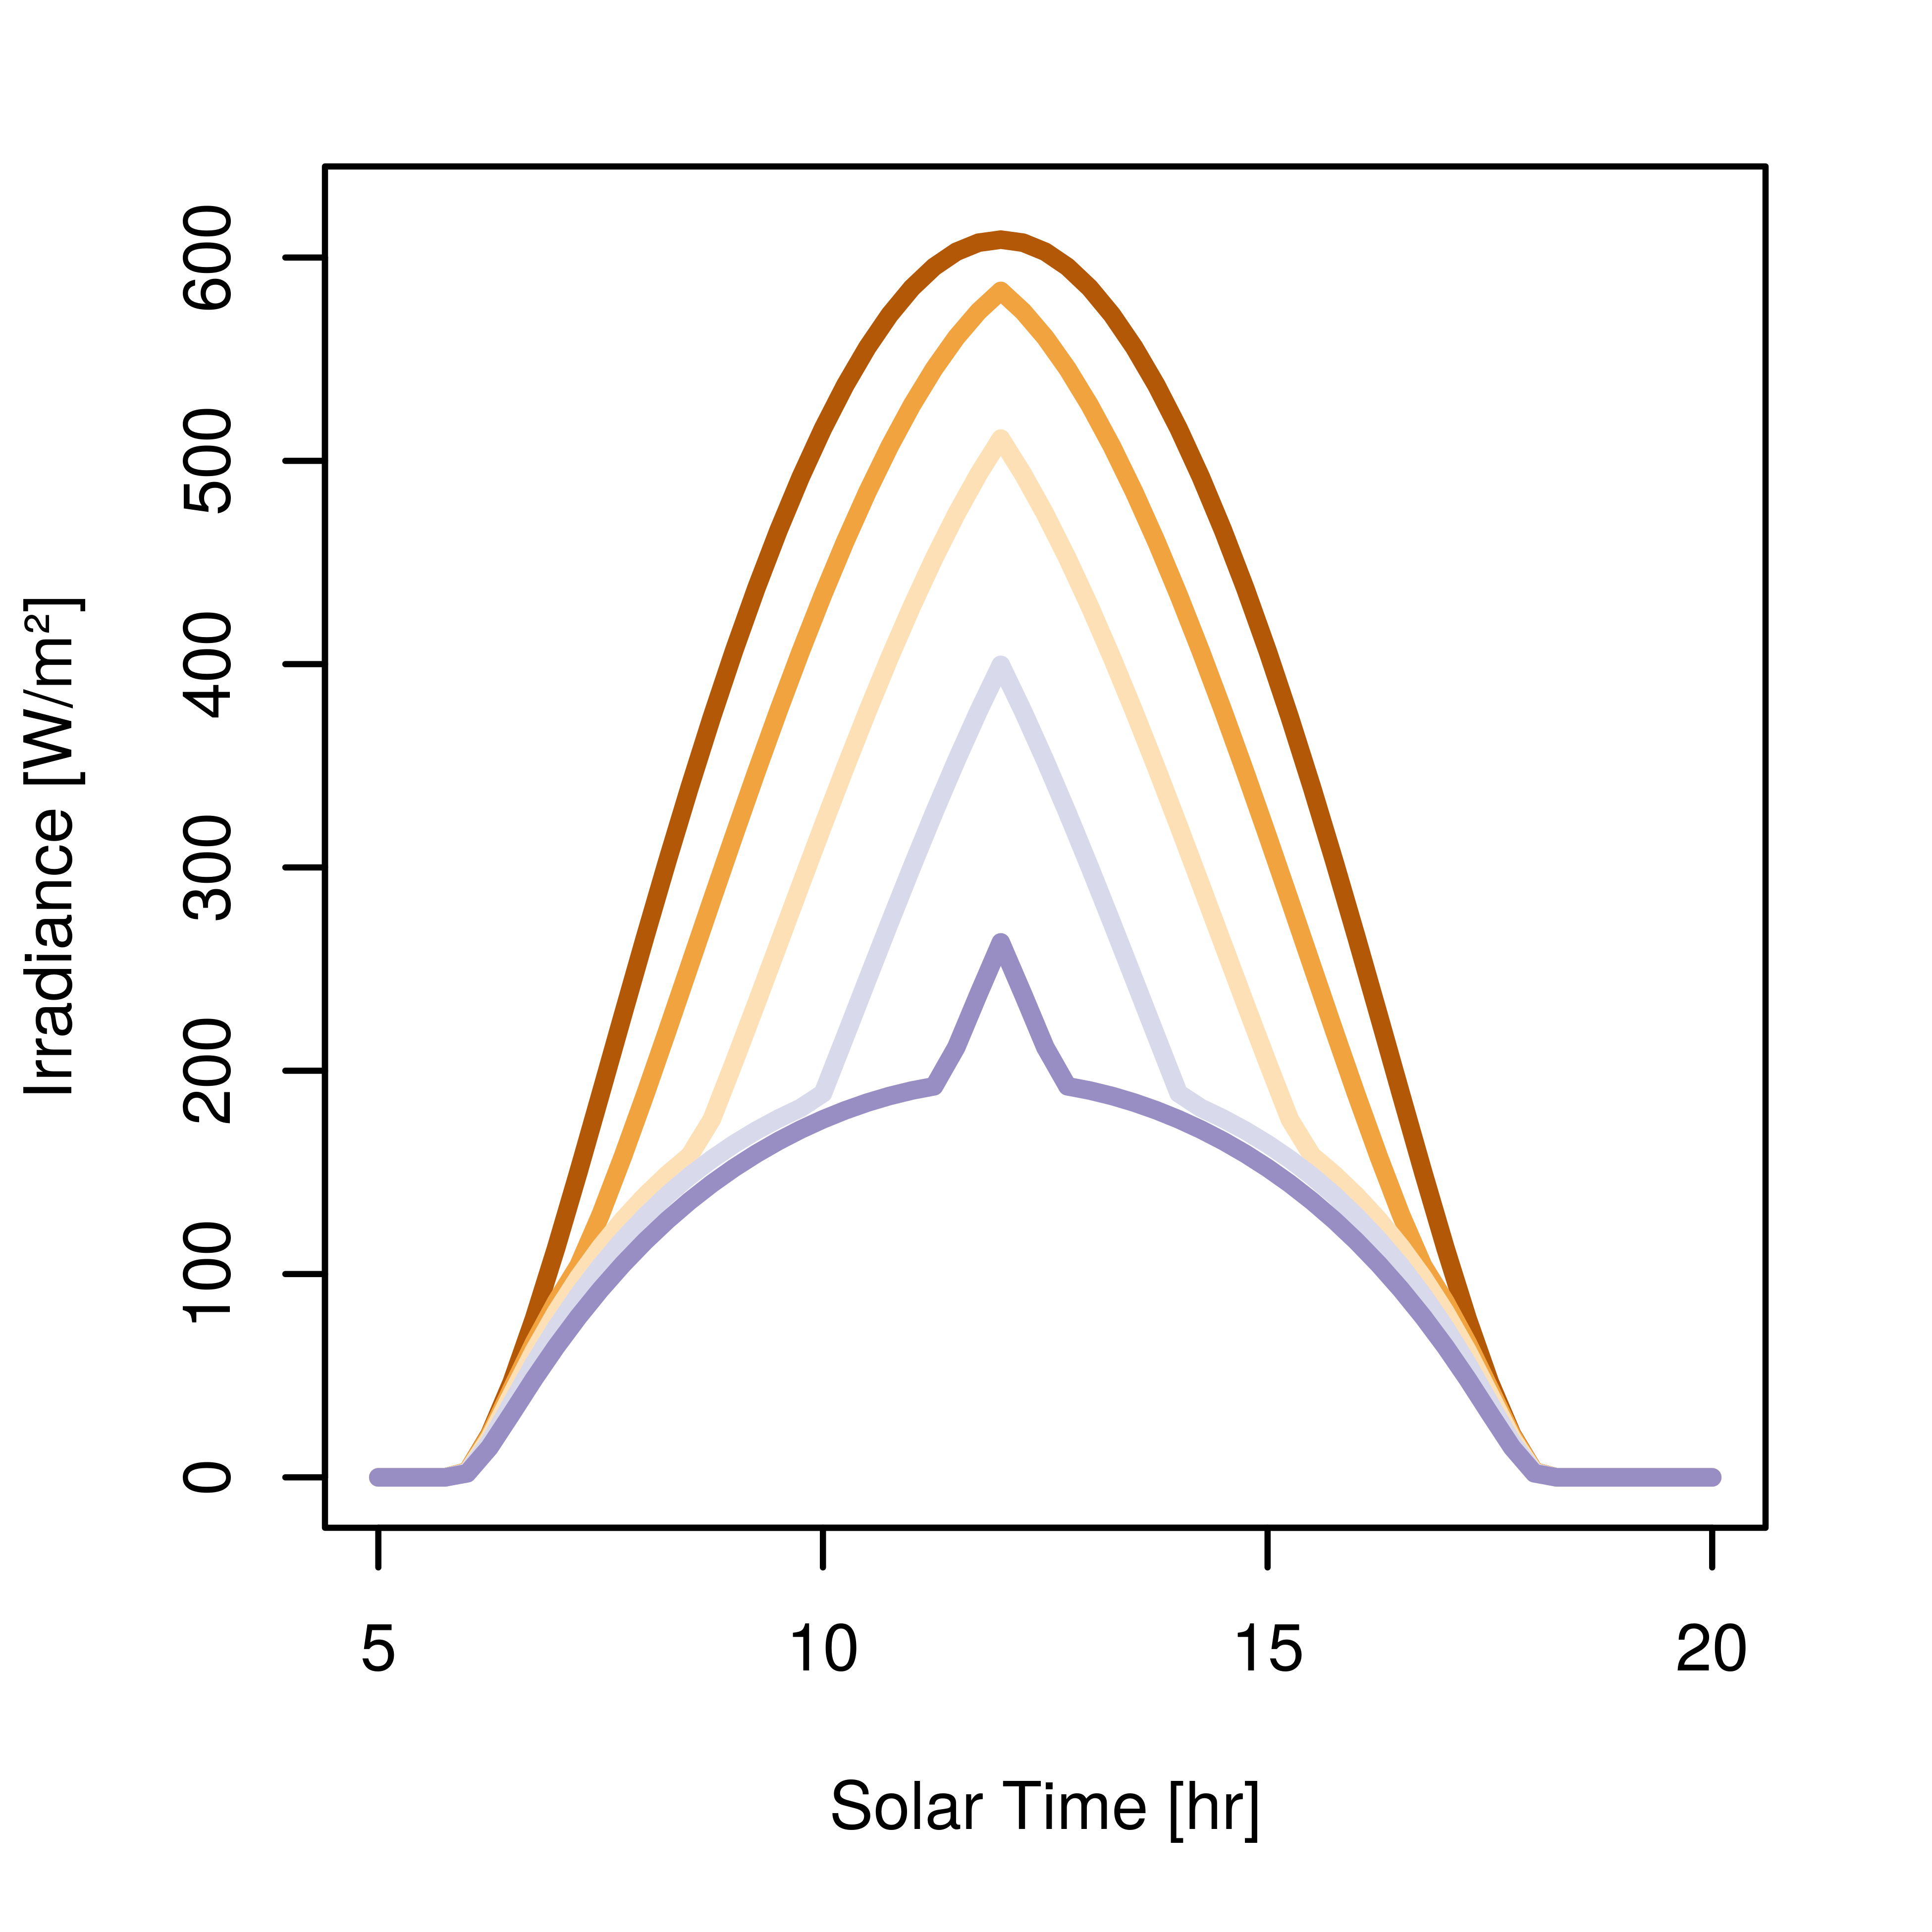
\includegraphics[height=\graphicsHeight]{sections/mars-solar-energy/solar-radiation/plots/gi-variationfor-ls-248-phi-2-tau-05-gammac-east-and-albedo-027.png}
  		\subcaption{$\gamma_{c} = \SI{-90}{\degree}$ (East)}
  		\label{fig:sub:irradiance-inclined-gamma-c-m90}
  	\end{subfigure}\\[0.8ex]
%% 2nd row
    \begin{subfigure}[t]{\subfigureWidth}
      \centering
  		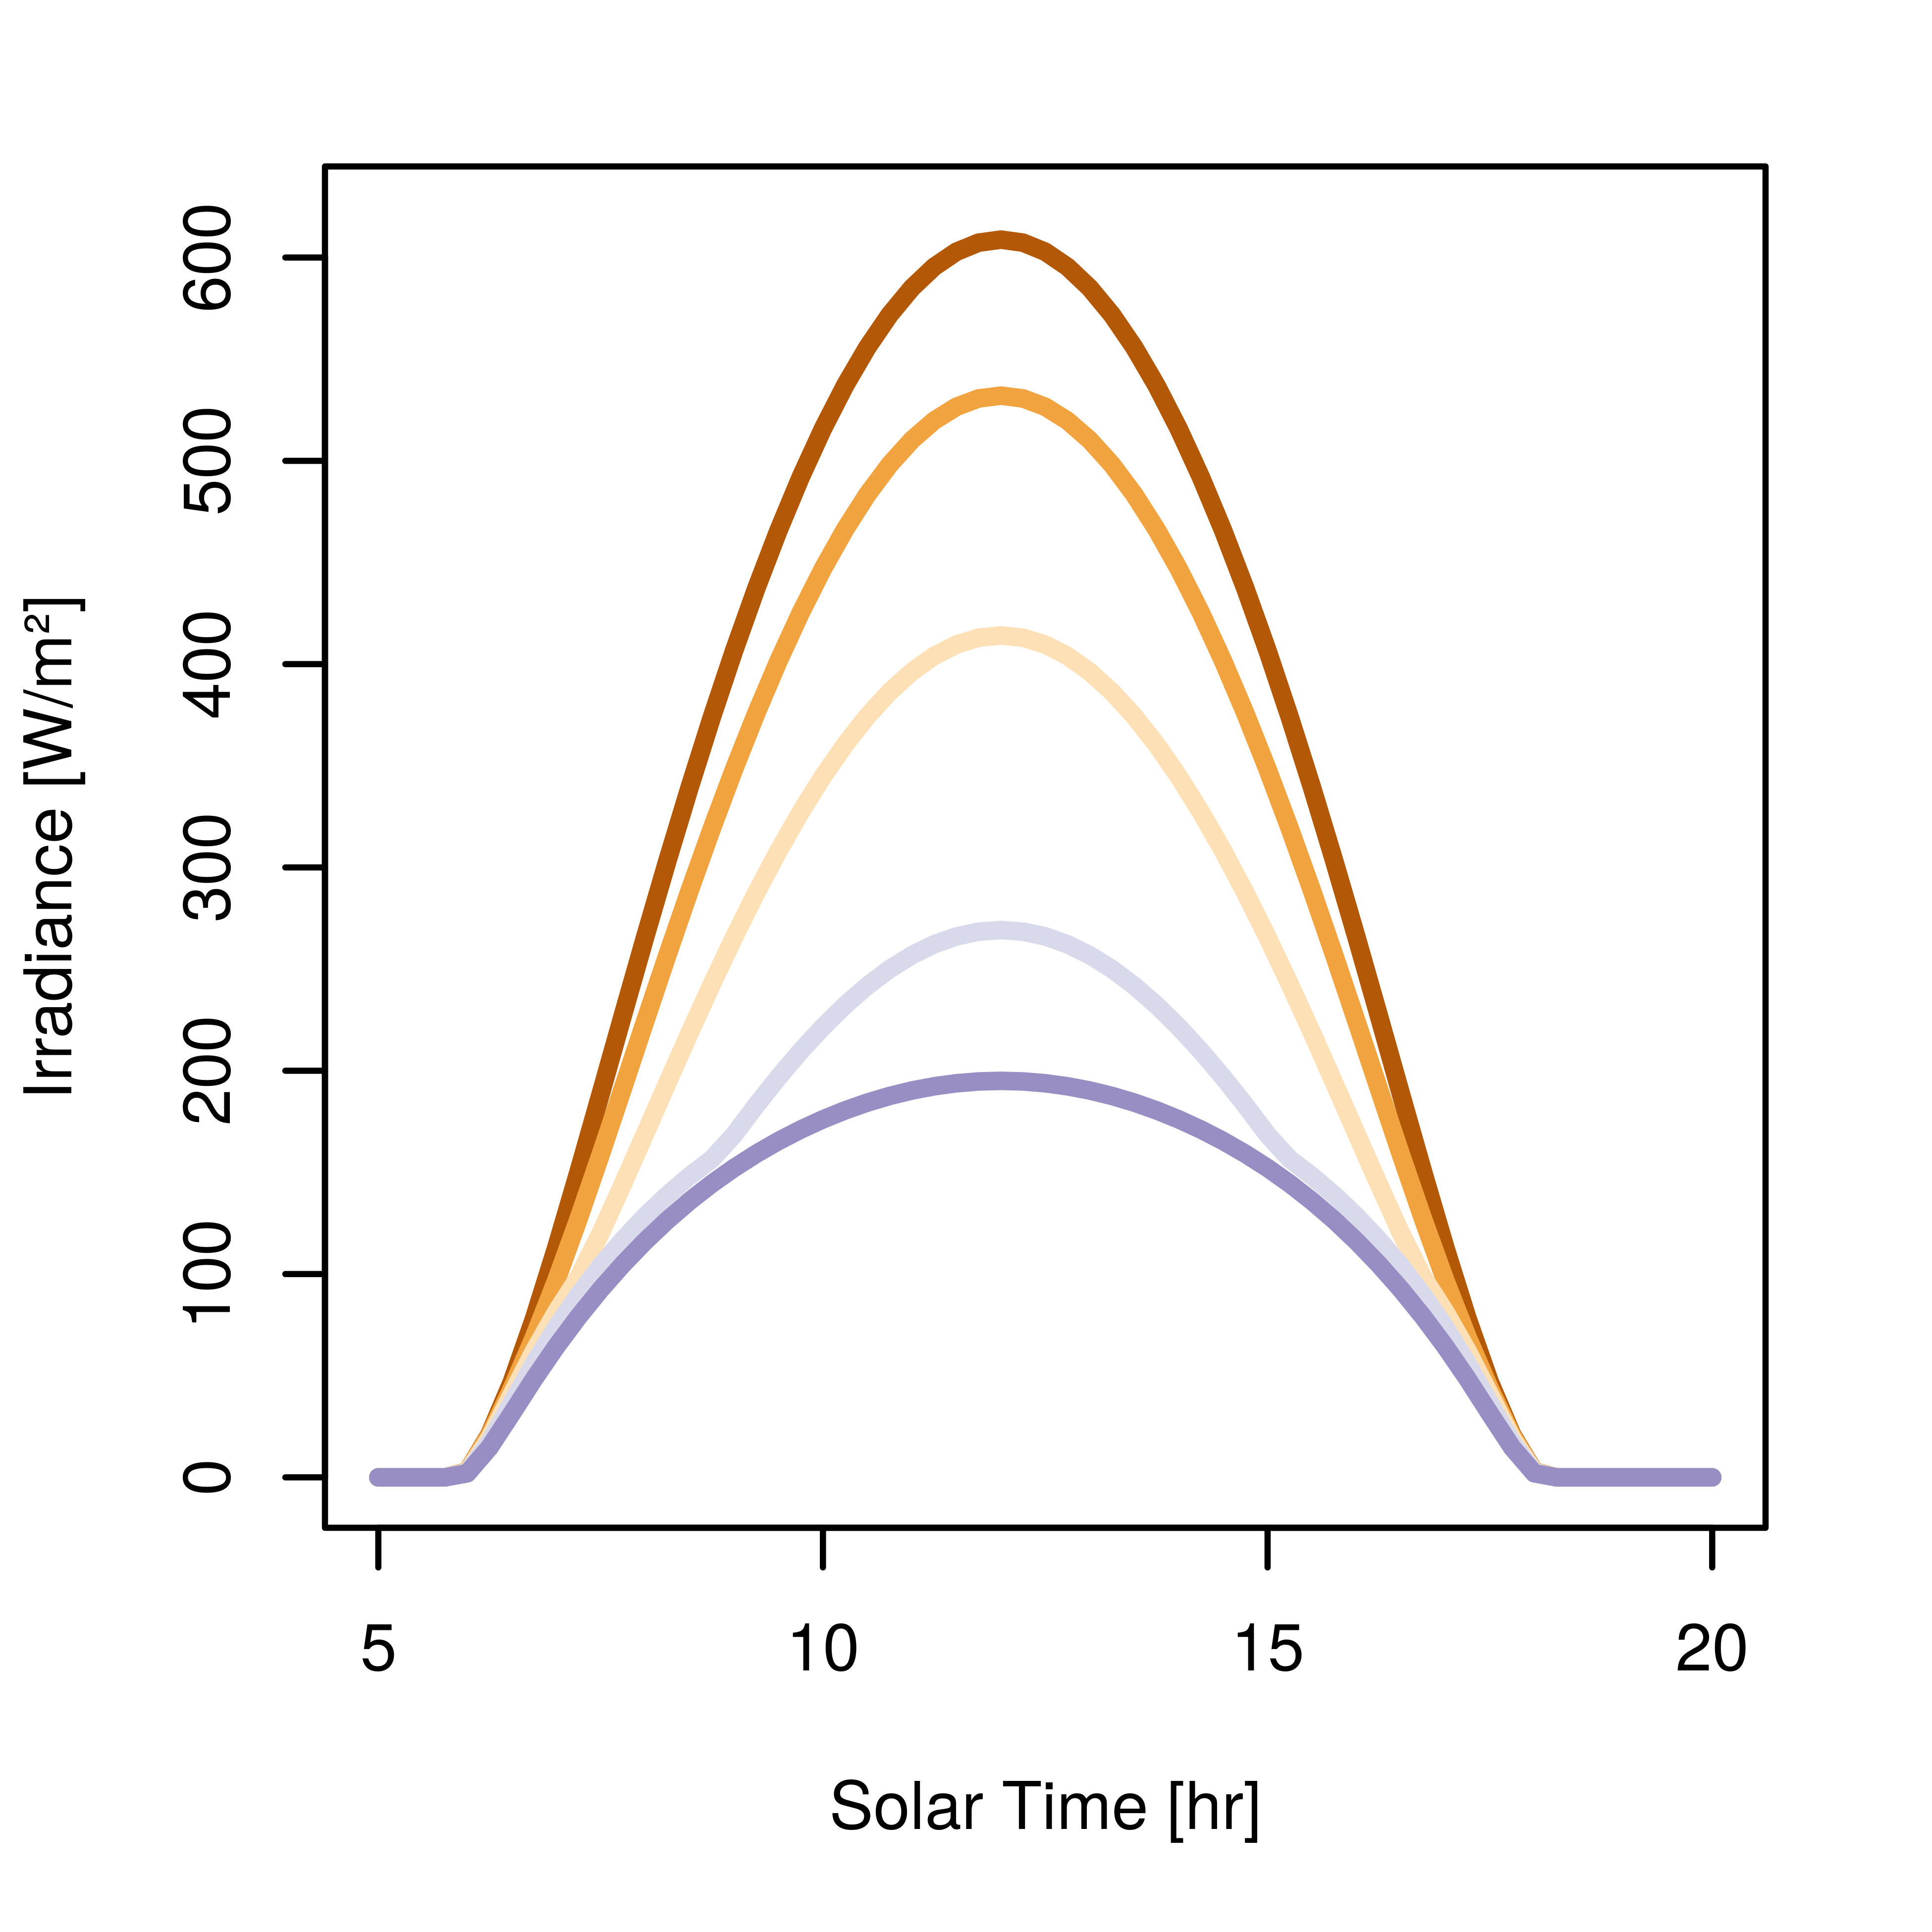
\includegraphics[height=\graphicsHeight]{sections/mars-solar-energy/solar-radiation/plots/gi-variationfor-ls-248-phi-2-tau-05-gammac-south-and-albedo-027.png}
  		\subcaption{$\gamma_{c} = \SI{-180}{\degree}$ (South)}
  		\label{fig:sub:irradiance-inclined-gamma-c-m180}
  	\end{subfigure}\hfill
	   \begin{subfigure}[t]{\subfigureWidth}
      \centering
  		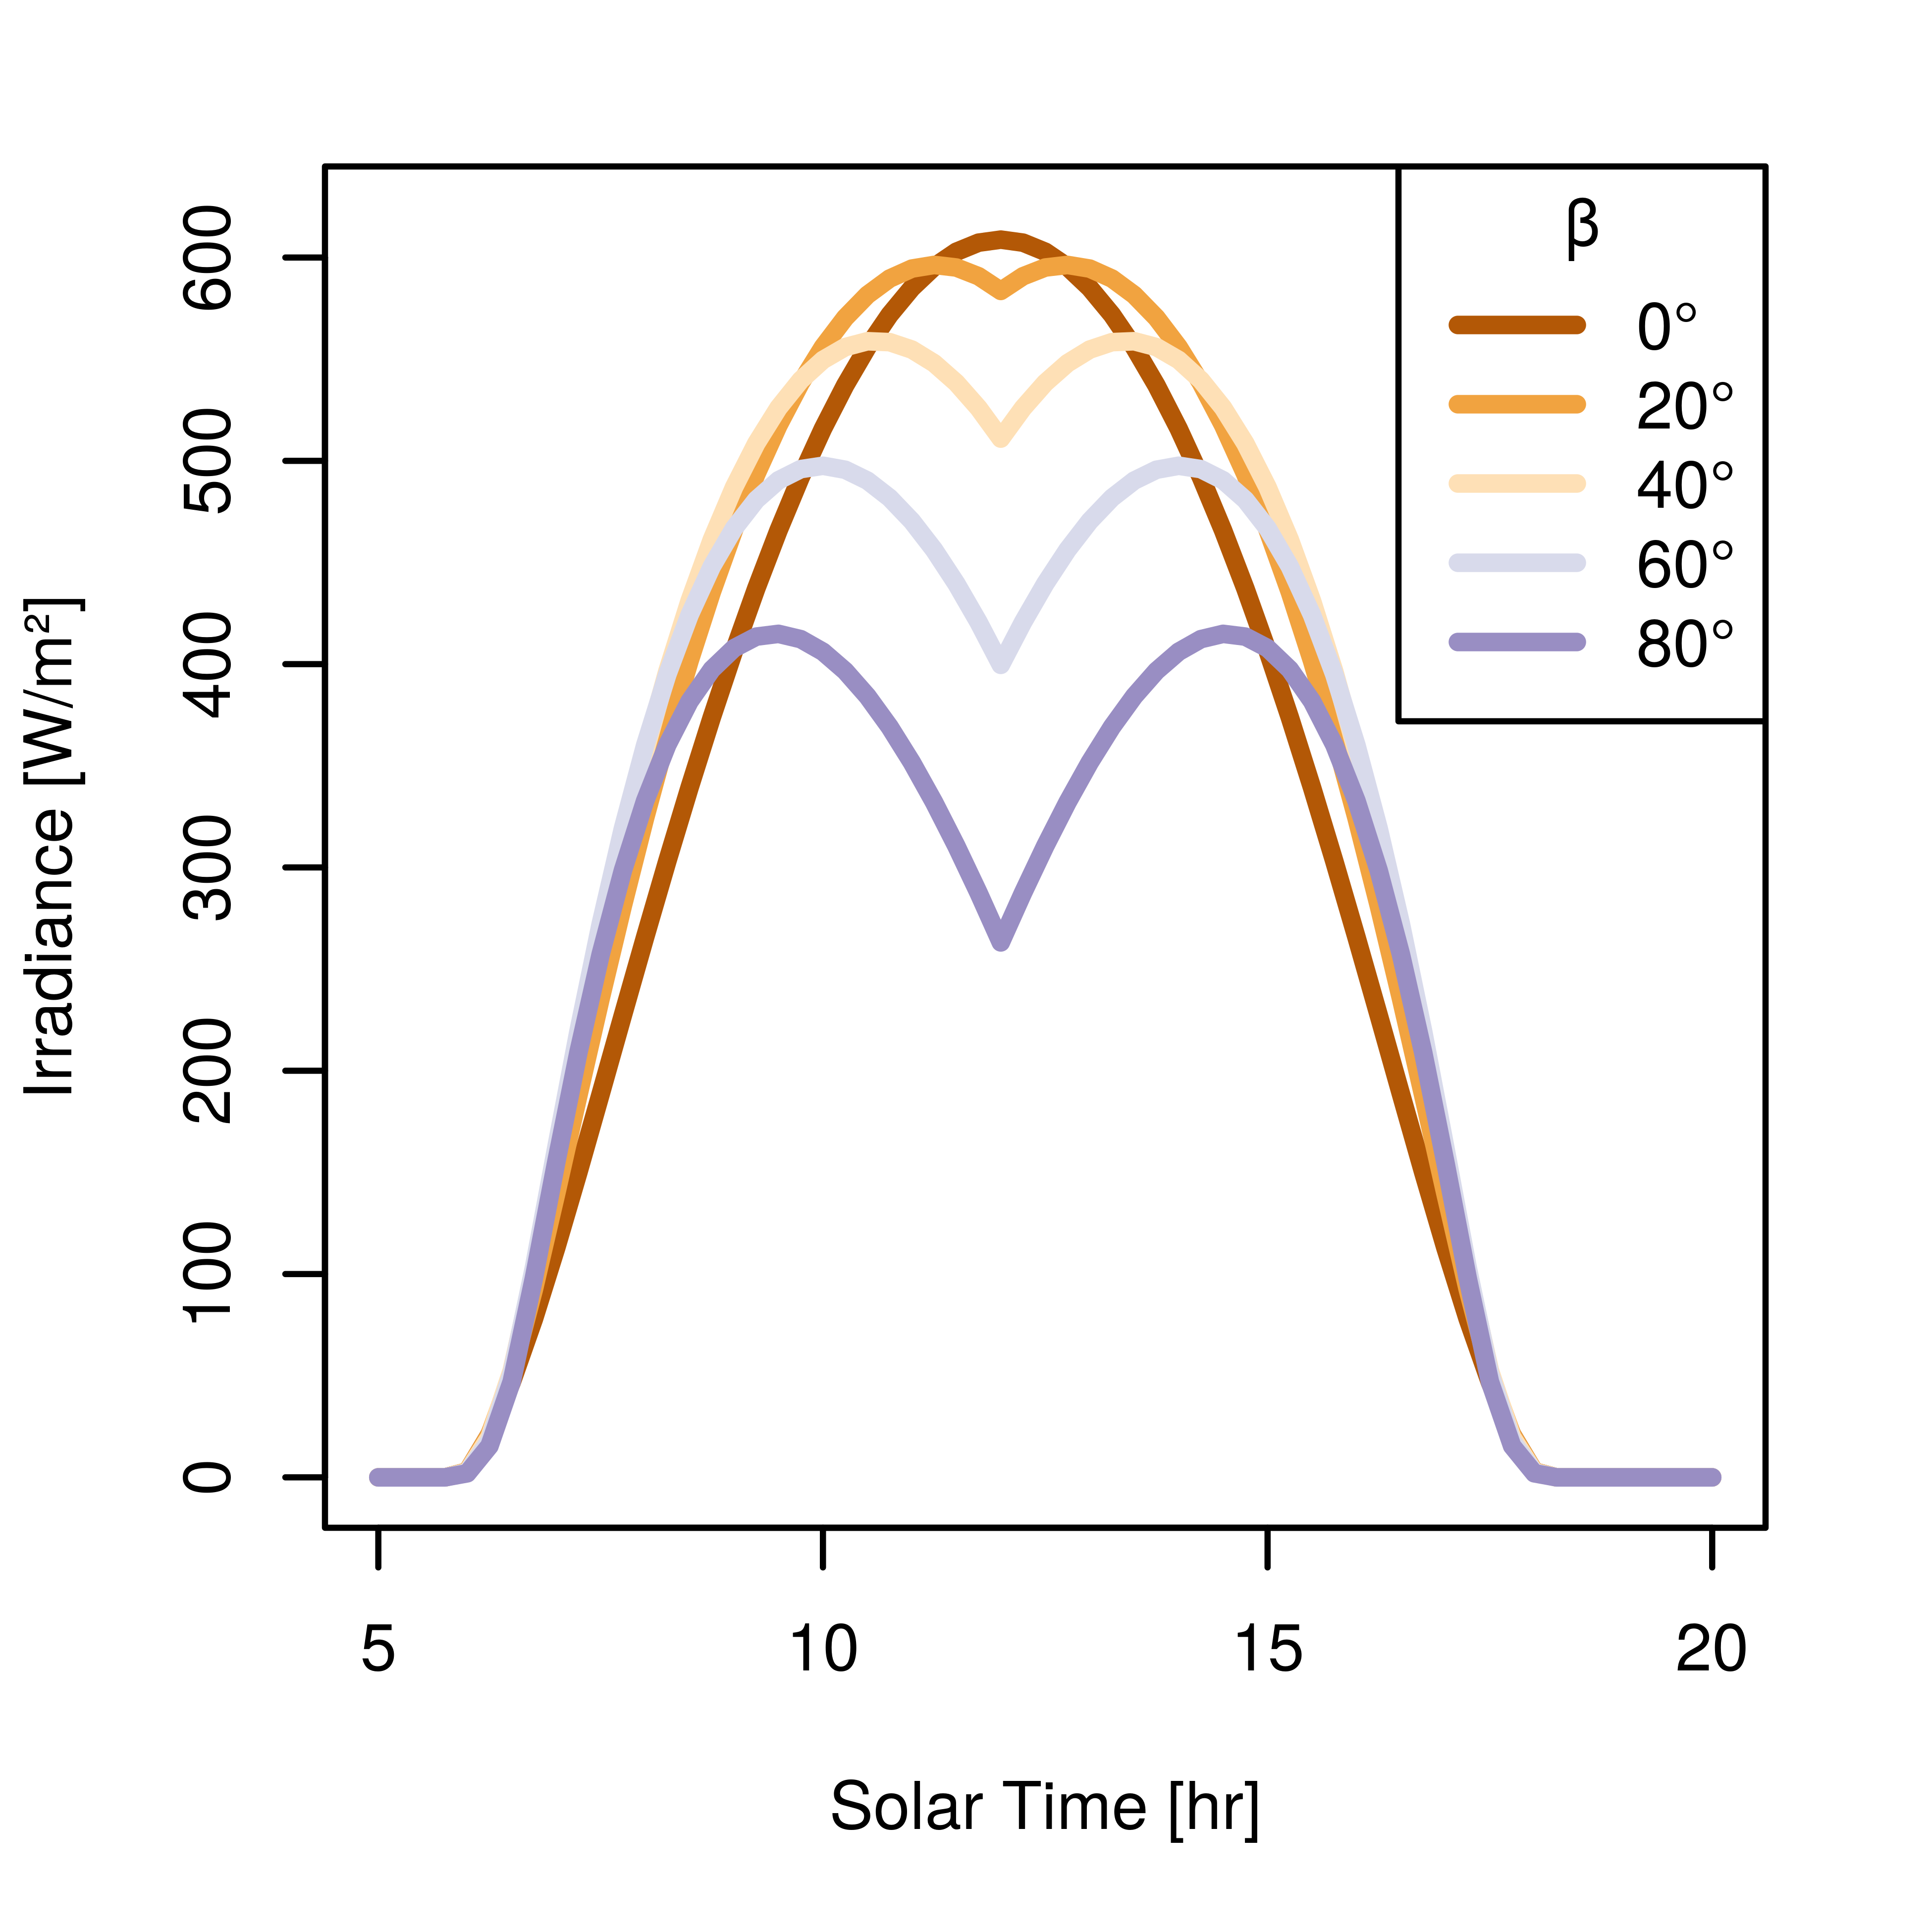
\includegraphics[height=\graphicsHeight]{sections/mars-solar-energy/solar-radiation/plots/gi-variationfor-ls-248-phi-2-tau-05-gammac-west-and-albedo-027.png}
  		\subcaption{$\gamma_{c} = \SI{90}{\degree}$ (West)}
  		\label{fig:sub:irradiance-inclined-gamma-c-90}
	   \end{subfigure}\hfill
	\caption{Diurnal variation of global irradiance on Mars inclined surface for different orientations when $L_{s} = \SI{248}{\degree}$, $\phi = \SI{-2}{\degree}$, and $\tau = \SI{0}{\degree}$.}
	\label{fig:plot:irradiance-inclined-gamma-c}
\vspace{-2ex}
\end{figure}

\clearpage
%\subsubsection{Insolation}
%\label{sec:MartianEnvironment:SolarRadiation:InclinedSurface:Insolation}

Global insolations on an inclined surface for a given time period $I_{\beta}$ and daily global insolation $H_{\beta}$ are obtained by following the same procedure described in Section \ref{sec:MartianEnvironment:SolarRadiation:Insolation}. That is to say, by integrating the $G_{\beta}$ irradiance Equation \ref{eq:G_beta} to obtain $I_{\beta}$ and integrating $I_{\beta}$ over the period from sunrise to sunset to obtain $H_{\beta}$.

%\todo[inline]{TODO: Present plots for diurnal variation of global insolation on Mars inclined surface for different orientations. This is obtained by integrating the global irradiance on Mars incline surface.}

\todo[inline]{\textbf{TODO:} Emphasize that it doesn't matter which inclination and orientation configuration you have when most of the irradiance is scattered (dusty days).}

\subsection{Summary}
\todo[inline]{\textbf{TODO:} Write section summary.}


\clearpage
\section{Photovoltaic Energy}
\label{sec:MarsSolarEnergy:PhotovoltaicEnergy}
\todo[inline]{\textbf{TODO:} Write section introduction.}

\subsection{Performance Ratio}
\label{sec:PowerAndEnergyPredictions:PerformanceRatio}
Power and energy calculations take into account solar cell performance ratio \ac{PR}, also known as the coefficient for losses. \ac{PR} components are taken from Mars \ac{PV} literature:

\begin{enumerate}[label=\textbf{\textcolor{BulletBlue}{(\alph*)}}]
  \item\label{itm:pr:perm_loss}After deployment, \SI{5}{\percent} permanent dust power loss \citepower{McNatt2016}.
  \item\label{itm:pr:temp}Solar cell efficiency varies by \SI{3}{\percent} due to changing temperature and red-shift spectral losses through the day time-period \citepower{Kerslake1999}.
  \item\label{itm:pr:deposition}Dust deposition degrade the performance at a rate of \SI{0.28}{\percent} per sol during the initial 30 Sols of a mission and long-term degradation is about \SI{0.14}{\percent} per sol \citepower{Landis2004}.
  \item\label{itm:pr:saturation}Dust performance degradiation saturates at about \SI{30}{\percent} \citepower{Stella2005}.
  \item\label{itm:pr:shadowing}Variable shadowing from protruding rover structures \citepower{Stella2005} and terrain masking \citepower{Kerslake1999}.
\end{enumerate}

The components used for \ac{PR} in the daily energy calculations throughout this chapter will initially be made up of degradation coefficients from \ref{itm:pr:perm_loss} and \ref{itm:pr:temp} where validation against \ac{MER} Opportunity data will use the solar array dust factor reported by the rover rather than those described in \ref{itm:pr:deposition} and \ref{itm:pr:saturation}. Losses from \ref{itm:pr:shadowing} and other unaccounted factors will be initially assumed at \SI{5}{\percent} and then iteratively revised along with the solar array dust factor so that the error margin range may be reduced.

Dust deposition induced losses do not perennially degrade the solar cells but fluctuate due to probabilistic dust cleaning events such as encounters with dust devils, storm winds, or even from a steep tilt angle as seen in Figure \ref{fig:image:mer-opportunity-dust-streaks}.

\begin{figure}[h]
  \centering
  \hypersetup{linkcolor=captionTextColor}
  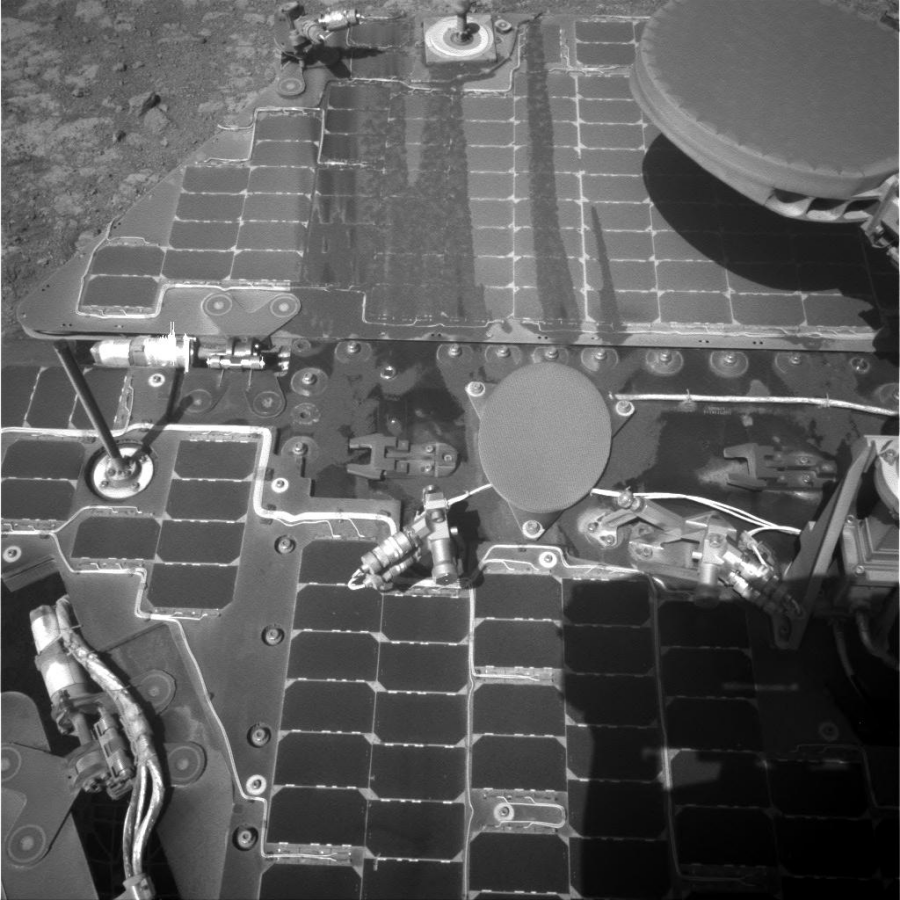
\includegraphics[width=0.5\linewidth]{sections/mars-solar-energy/photovoltaic-energy/images/mer-opportunity-dust-streaks.png}\\
  \caption[Streak of dust on \ac{MER} Opportunity's rear solar array during a steep tilt]
          {During a forward, uphill drive on Sol 4311 (March 10, 2016), Opportunity's tilt reached \SI{32}{\degree}. Vibrations from wheels slipping against the ground caused dust to streak down from \ac{MER} Opportunity's rear solar array while the rover was steeply tilted. Image taken on Sol 4322 (March 21, 2016). Image: \ac{NASA}/\ac{JPL}-Caltech.}
  \label{fig:image:mer-opportunity-dust-streaks}
\end{figure}
% Source: https://www.nasa.gov/feature/jpl/rover-takes-on-steepest-slope-ever-tried-on-mars

\subsection{Predictions}
\label{sec:PowerAndEnergyPredictions:Predictions}

The power output $P$ generated from a photovoltaic system is measured in watts (\si{\watt}) and is obtained from the global irradiance $G_{h}$ captured by its solar cells:

\begin{equation}
  \label{eq:SA_power}
  P = A \cdot \eta \cdot G_{h} \cdot PR
\end{equation}

where $A$ is the solar cell coverage area $\eta$ their efficiency.

The generated daily energy output $E$ is measured in watt-hours (\si{\watt\hour}) and is obtained from the daily global insolation $H_{h}$ captured by solar cells:

\begin{equation}
  \label{eq:SA_energy}
  E = A \cdot \eta \cdot H_{h} \cdot PR
\end{equation}

Power and energy calculations for inclined solar arrays are obtained from $G_{\beta}$ and $I_{\beta}$. They are denoted as $P_{\beta}$ and $E_{\beta}$ respectively:

\begin{equation}
  \label{eq:SA_slope_power}
  P_{\beta} = A \cdot \eta \cdot G_{\beta} \cdot PR
\end{equation}


\begin{equation}
  \label{eq:SA_slope_energy}
  E_{\beta} = A \cdot \eta \cdot H_{\beta} \cdot PR
\end{equation}

It is worth emphasizing the difference between \ac{PV} cell, panel/module, and array surface areas in order to emphasize the correct parameter when calculating generated power and energy. \ac{PV} cells are interconnected together in a package called a panel, or module, which is then wired in series and parallel into a PV array. The interconnections between cells and wiring between panels introduce cell coverage gaps from which no power is generated. As such, considering panel or array rather than cell surface area for power and energy calculations would result in over-estimated values. By way of example, we consider the solar arrays on MER rovers in Figure \ref{fig:image:mer-solar-arrays} which is made up of a total of 499 cells: 165 on the port wing, 167 on the starboard wing, 102 on the stern, and 65 on the body. A cell's dimension is $\SI{3.95}{\centi\meter} \times \SI{6.89}{\centi\meter}$ with two cropped corners. This provides an active area of \SI{26.6}{\centi\meter\squared} thus the solar cell coverage area is $499 \times \SI{26.6}{\centi\meter\squared} = \SI{1.3}{\meter\squared}$.

\todo[inline]{\text{TODO:} Source E-mail exchange with Richard C. Ewell (NASA/JPL) for the MER solar cell size.}

\begin{figure}[h]
  \centering
  \hypersetup{linkcolor=captionTextColor}
  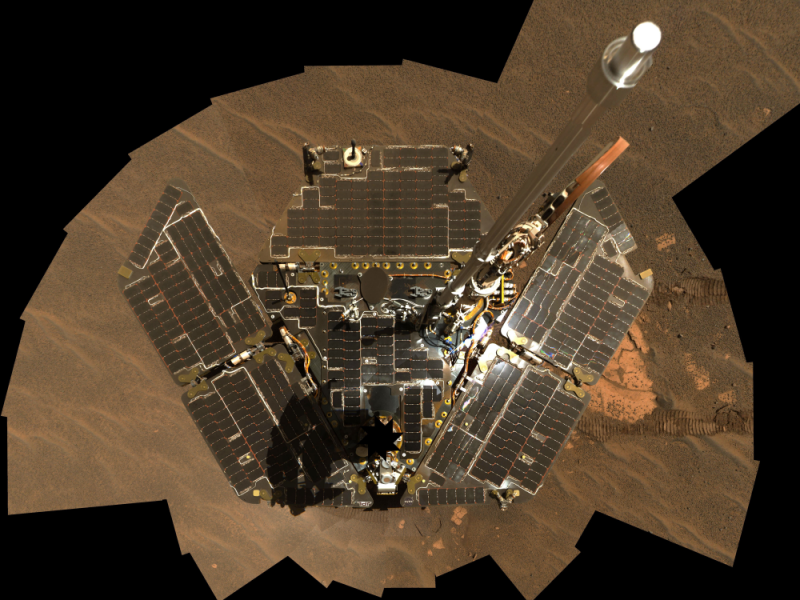
\includegraphics[width=0.8\linewidth]{sections/mars-solar-energy/photovoltaic-energy/images/mer-solar-arrays.png}\\
  \caption[\ac{MER} solar arrays]
          {\ac{MER} solar arrays. Image: \ac{NASA}/\ac{JPL}-Caltech/Cornell.}
  \label{fig:image:mer-solar-arrays}
\end{figure}
% Source: https://mars.nasa.gov/resources/5852/opportunity-self-portrait/?site=insight

\subsection{Validation}
\label{sec:PowerAndEnergyPredictions:Validation}
\todo[inline]{\textbf{TODO:} Write section introduction.}

%\todo[inline]{TODO: Short intro text? Why are we validating? Explain that the equations we are using were based on Viking Lander data and we need to verify if it is still robust today by validating it against the wealth of data we've accumulated since, specifically with MER Opportunity data which is illustrative of mobile rover missions rather than a stationary lander mission.}

\subsubsection{Horizontal Surface}
\label{sec:PowerAndEnergyPredictions:Validation:HorizontalSurface}

In order to validate the formulas presented in Section \ref{sec:PowerAndEnergyPredictions:Predictions}, \ac{MER} Opportunity status update parameters were applied to the daily energy calculation presented in Equation \ref{eq:SA_energy}. The following data was scraped from the rover's status update website for Mars years MY29 through MY33:

\begin{enumerate}[label=\textbf{\textcolor{BulletBlue}{(\alph*)}}]
  \item Sol: the mission's Martian day when the status report was made.
  \item Terrestrial date: the date on Earth when the status report was made.
  \item Atmospheric opacity: the $\tau$ factor introduced in Section \ref{sec:MartianEnvironment:Dust:AtmosphericOpacity}.
  \item Solar Array dust factor: a value between 0 and 1 with the latter represents perfectly clean solar arrays.
  \item Daily energy production: in watt-hours (\si{\watt\hour}).
\end{enumerate}

For the purpose of insolation calculations, the areocentric longitude $L_{s}$ was determined from the terrestrial date based on the process and equations in \citeother{Allison2000}. The resulting predicted energy production was then compared to the rover's reported daily energy production. These are presented for selected Mars years in Figure \ref{fig:plot:mer-energy-production-predicted-vs-reported}.

\begin{figure}[h]
\captionsetup[subfigure]{justification=centering}
\vspace{-2ex}
	\centering
    %% setup sizes
    \setlength{\subfigureWidth}{0.50\textwidth}
    \setlength{\graphicsHeight}{80mm}
    %% kill hyper-link highlighting
    \hypersetup{hidelinks=true}%
    %% the figures
%% 1st row
  	\begin{subfigure}[t]{\subfigureWidth}
      \centering
  		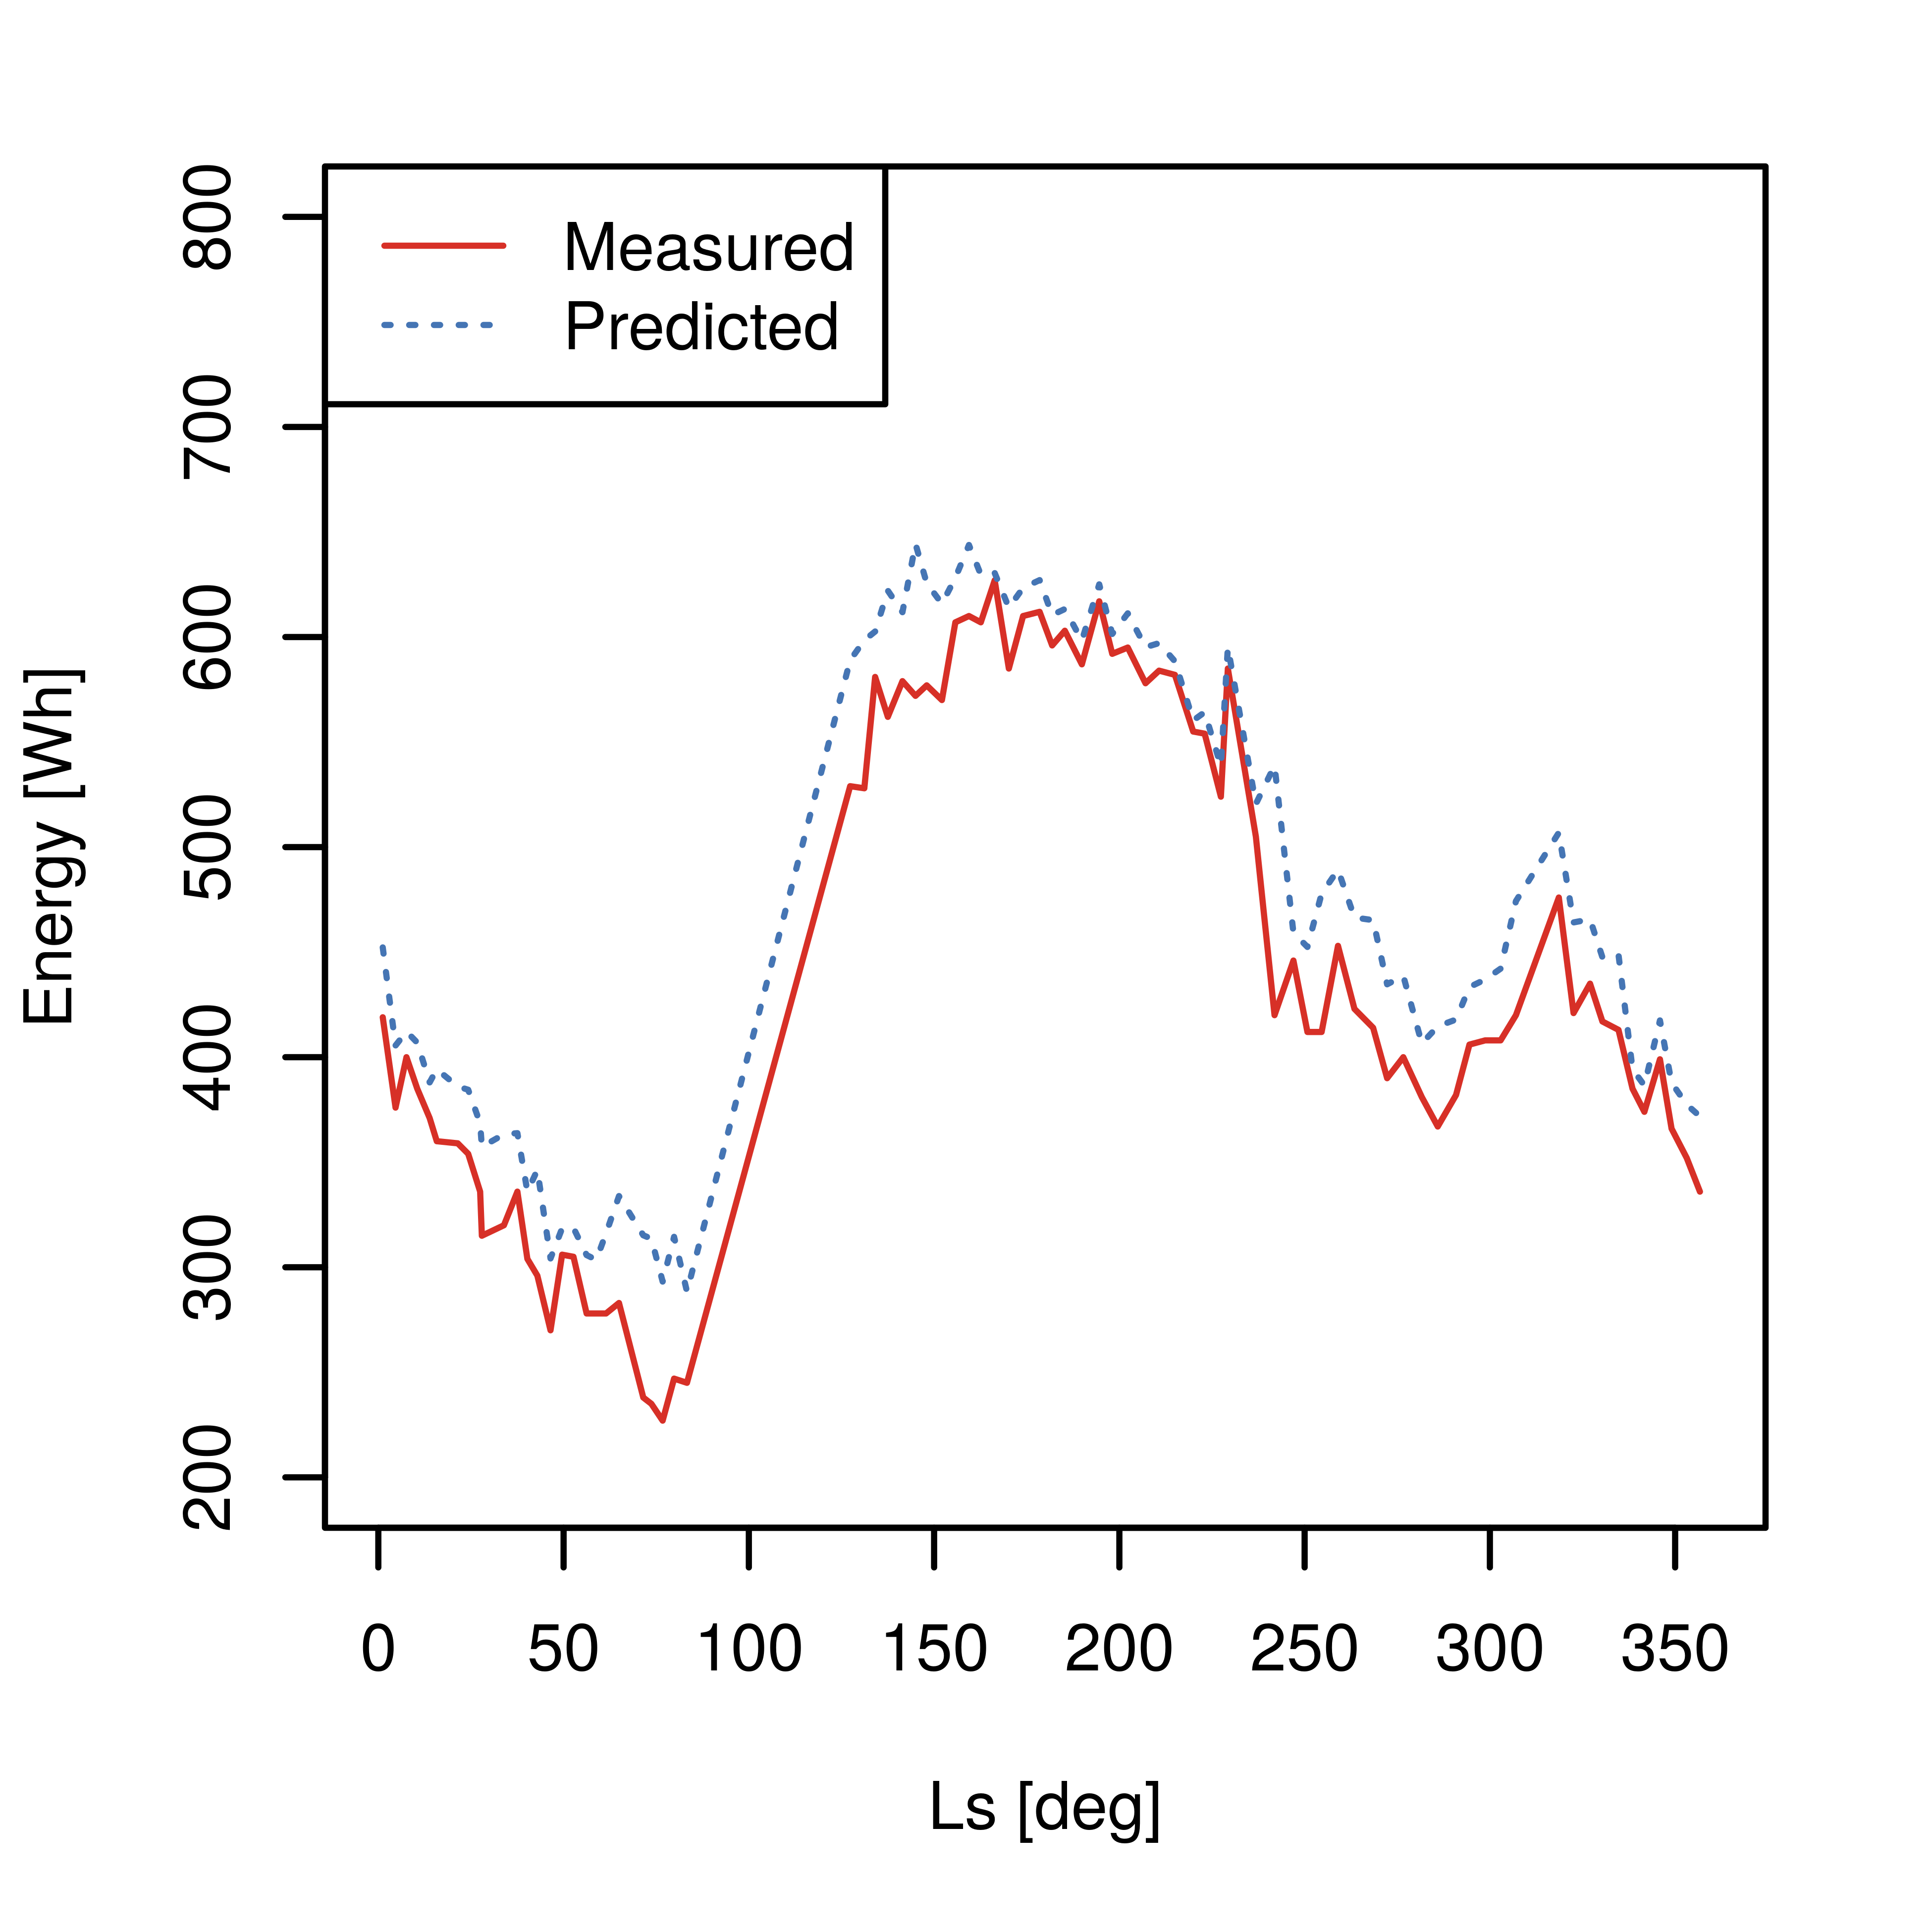
\includegraphics[height=\graphicsHeight]{sections/mars-solar-energy/photovoltaic-energy/plots/predicted-vs-measured-energy-my29.png}
  		\subcaption{MY29}
  		\label{fig:plot:sub:mer-energy-production-predicted-vs-reported-my29}
  	\end{subfigure}\hfill
    \begin{subfigure}[t]{\subfigureWidth}
      \centering
  		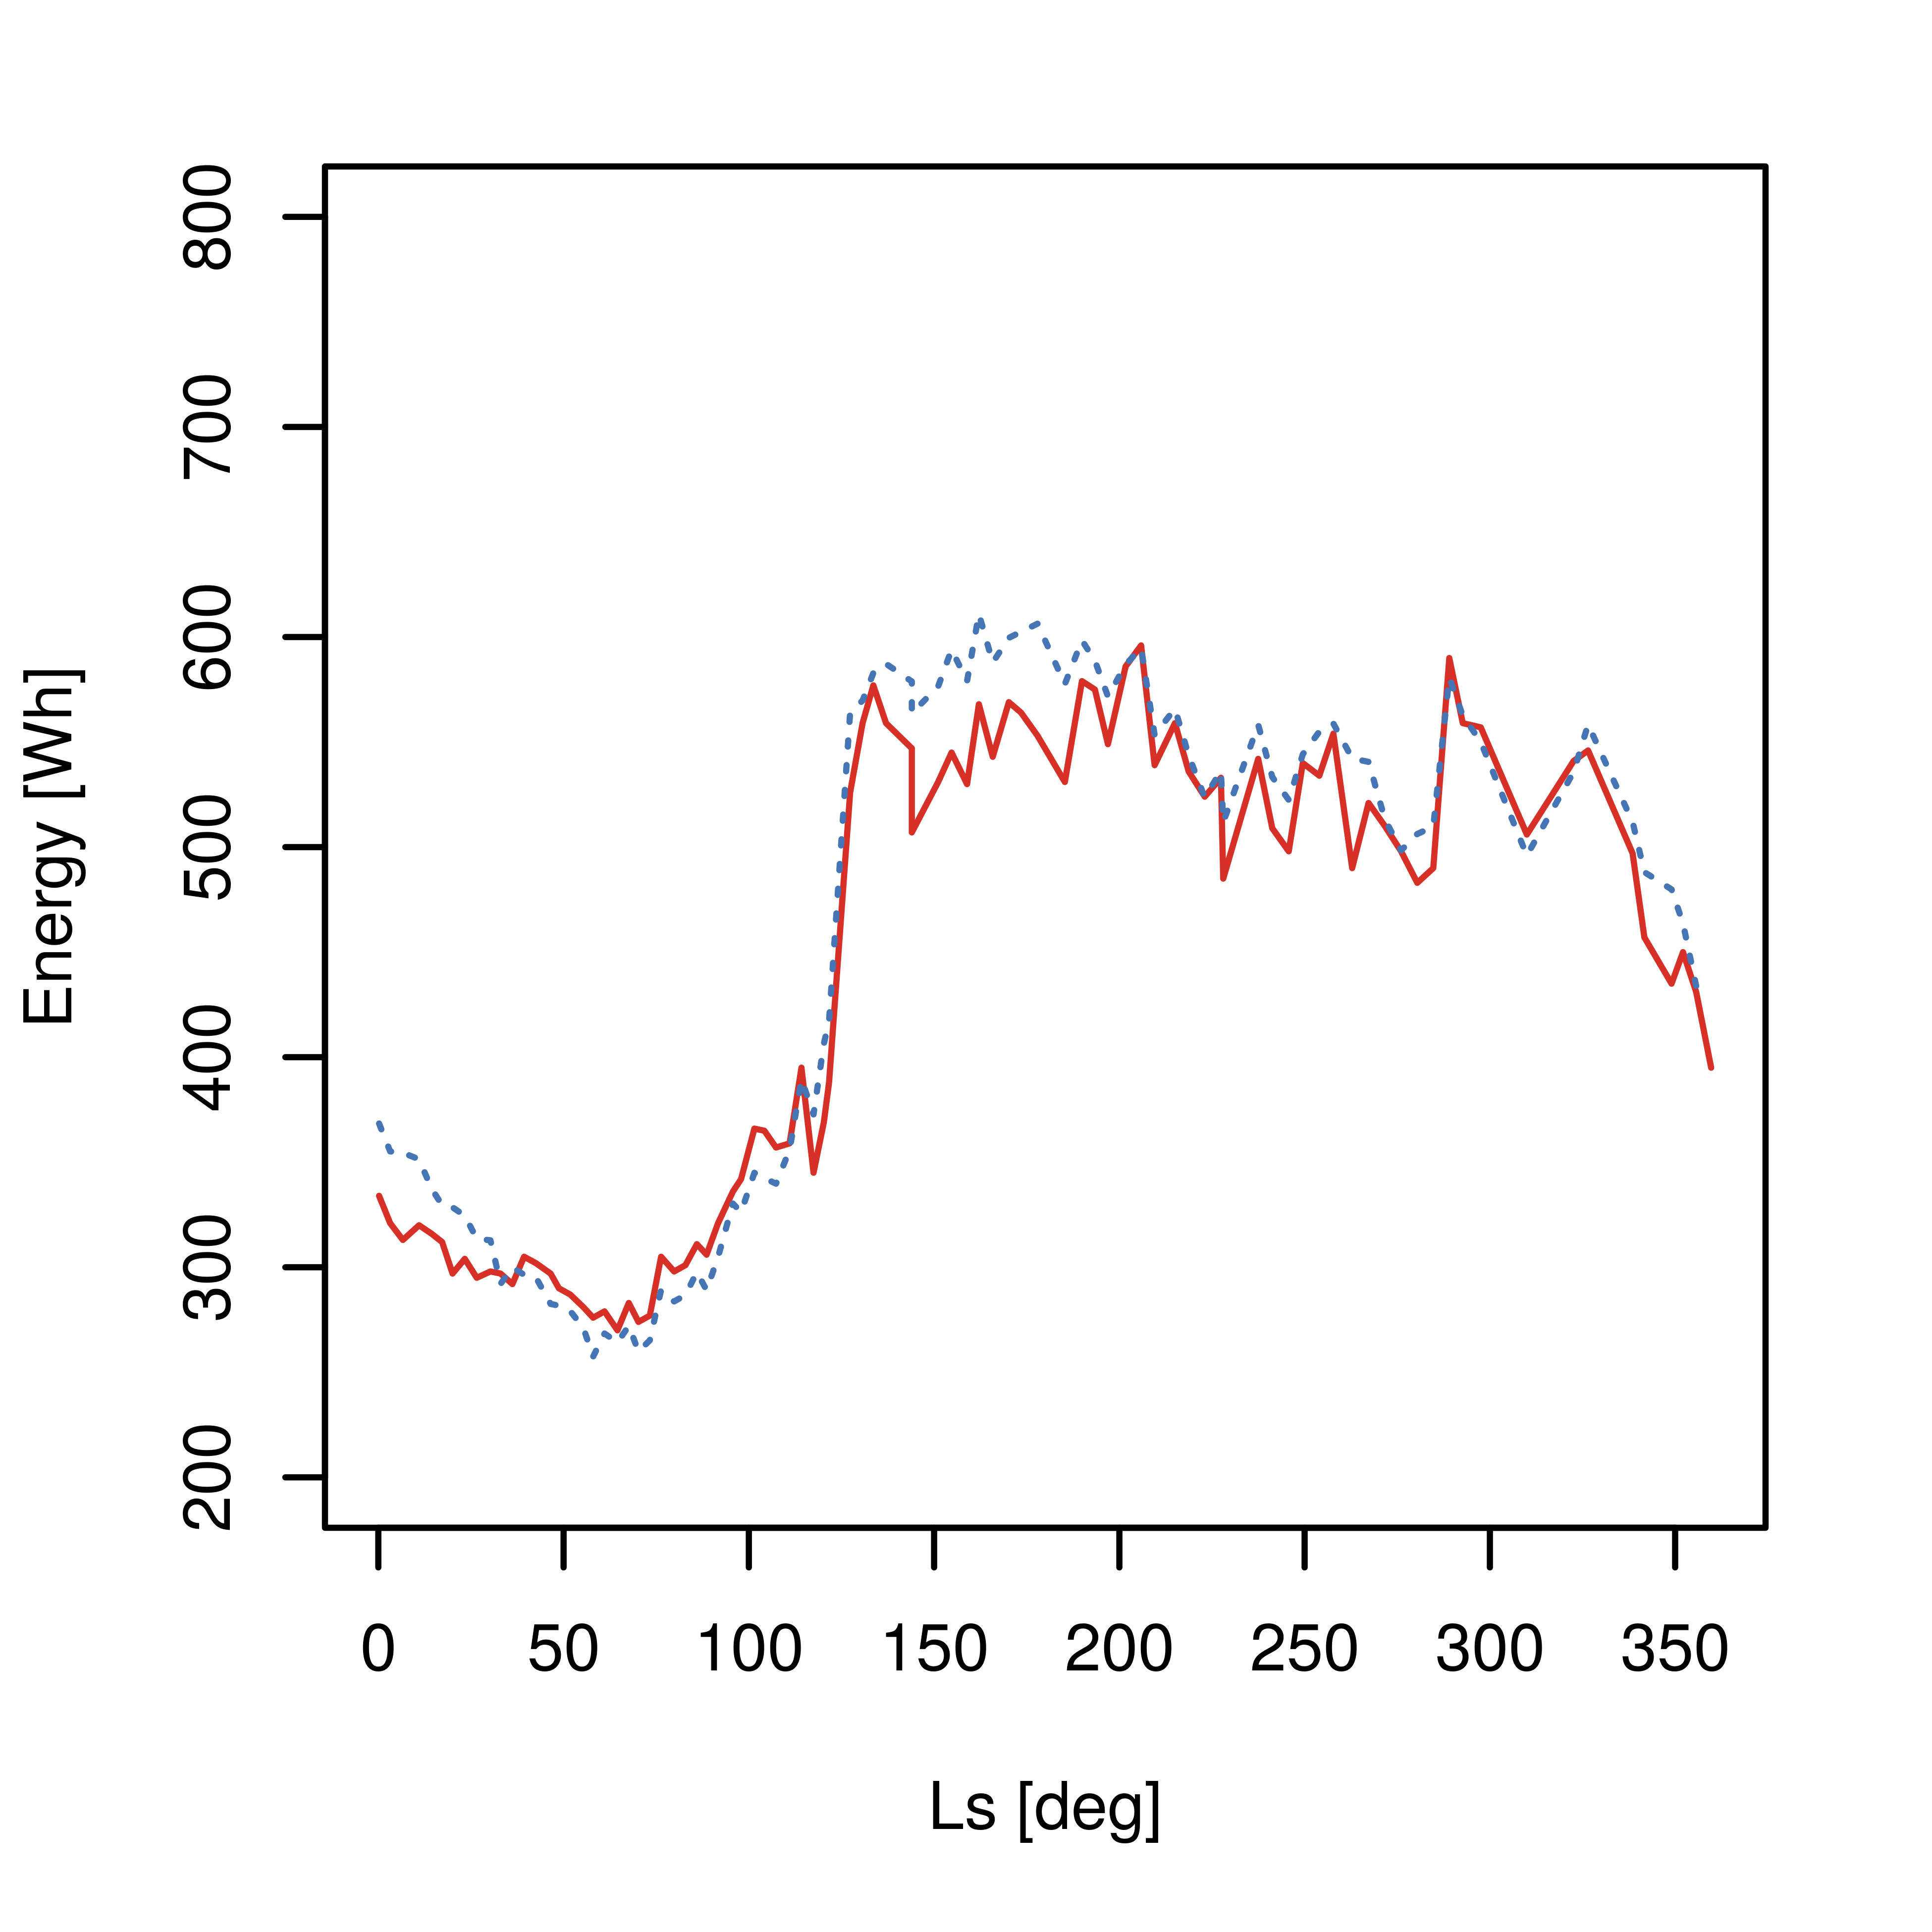
\includegraphics[height=\graphicsHeight]{sections/mars-solar-energy/photovoltaic-energy/plots/predicted-vs-measured-energy-my30.png}
  		\subcaption{MY30}
  		\label{fig:plot:sub:mer-energy-production-predicted-vs-reported-my30}
  	\end{subfigure}\\[0.8ex]
%% 2nd row
    \begin{subfigure}[t]{\subfigureWidth}
      \centering
  		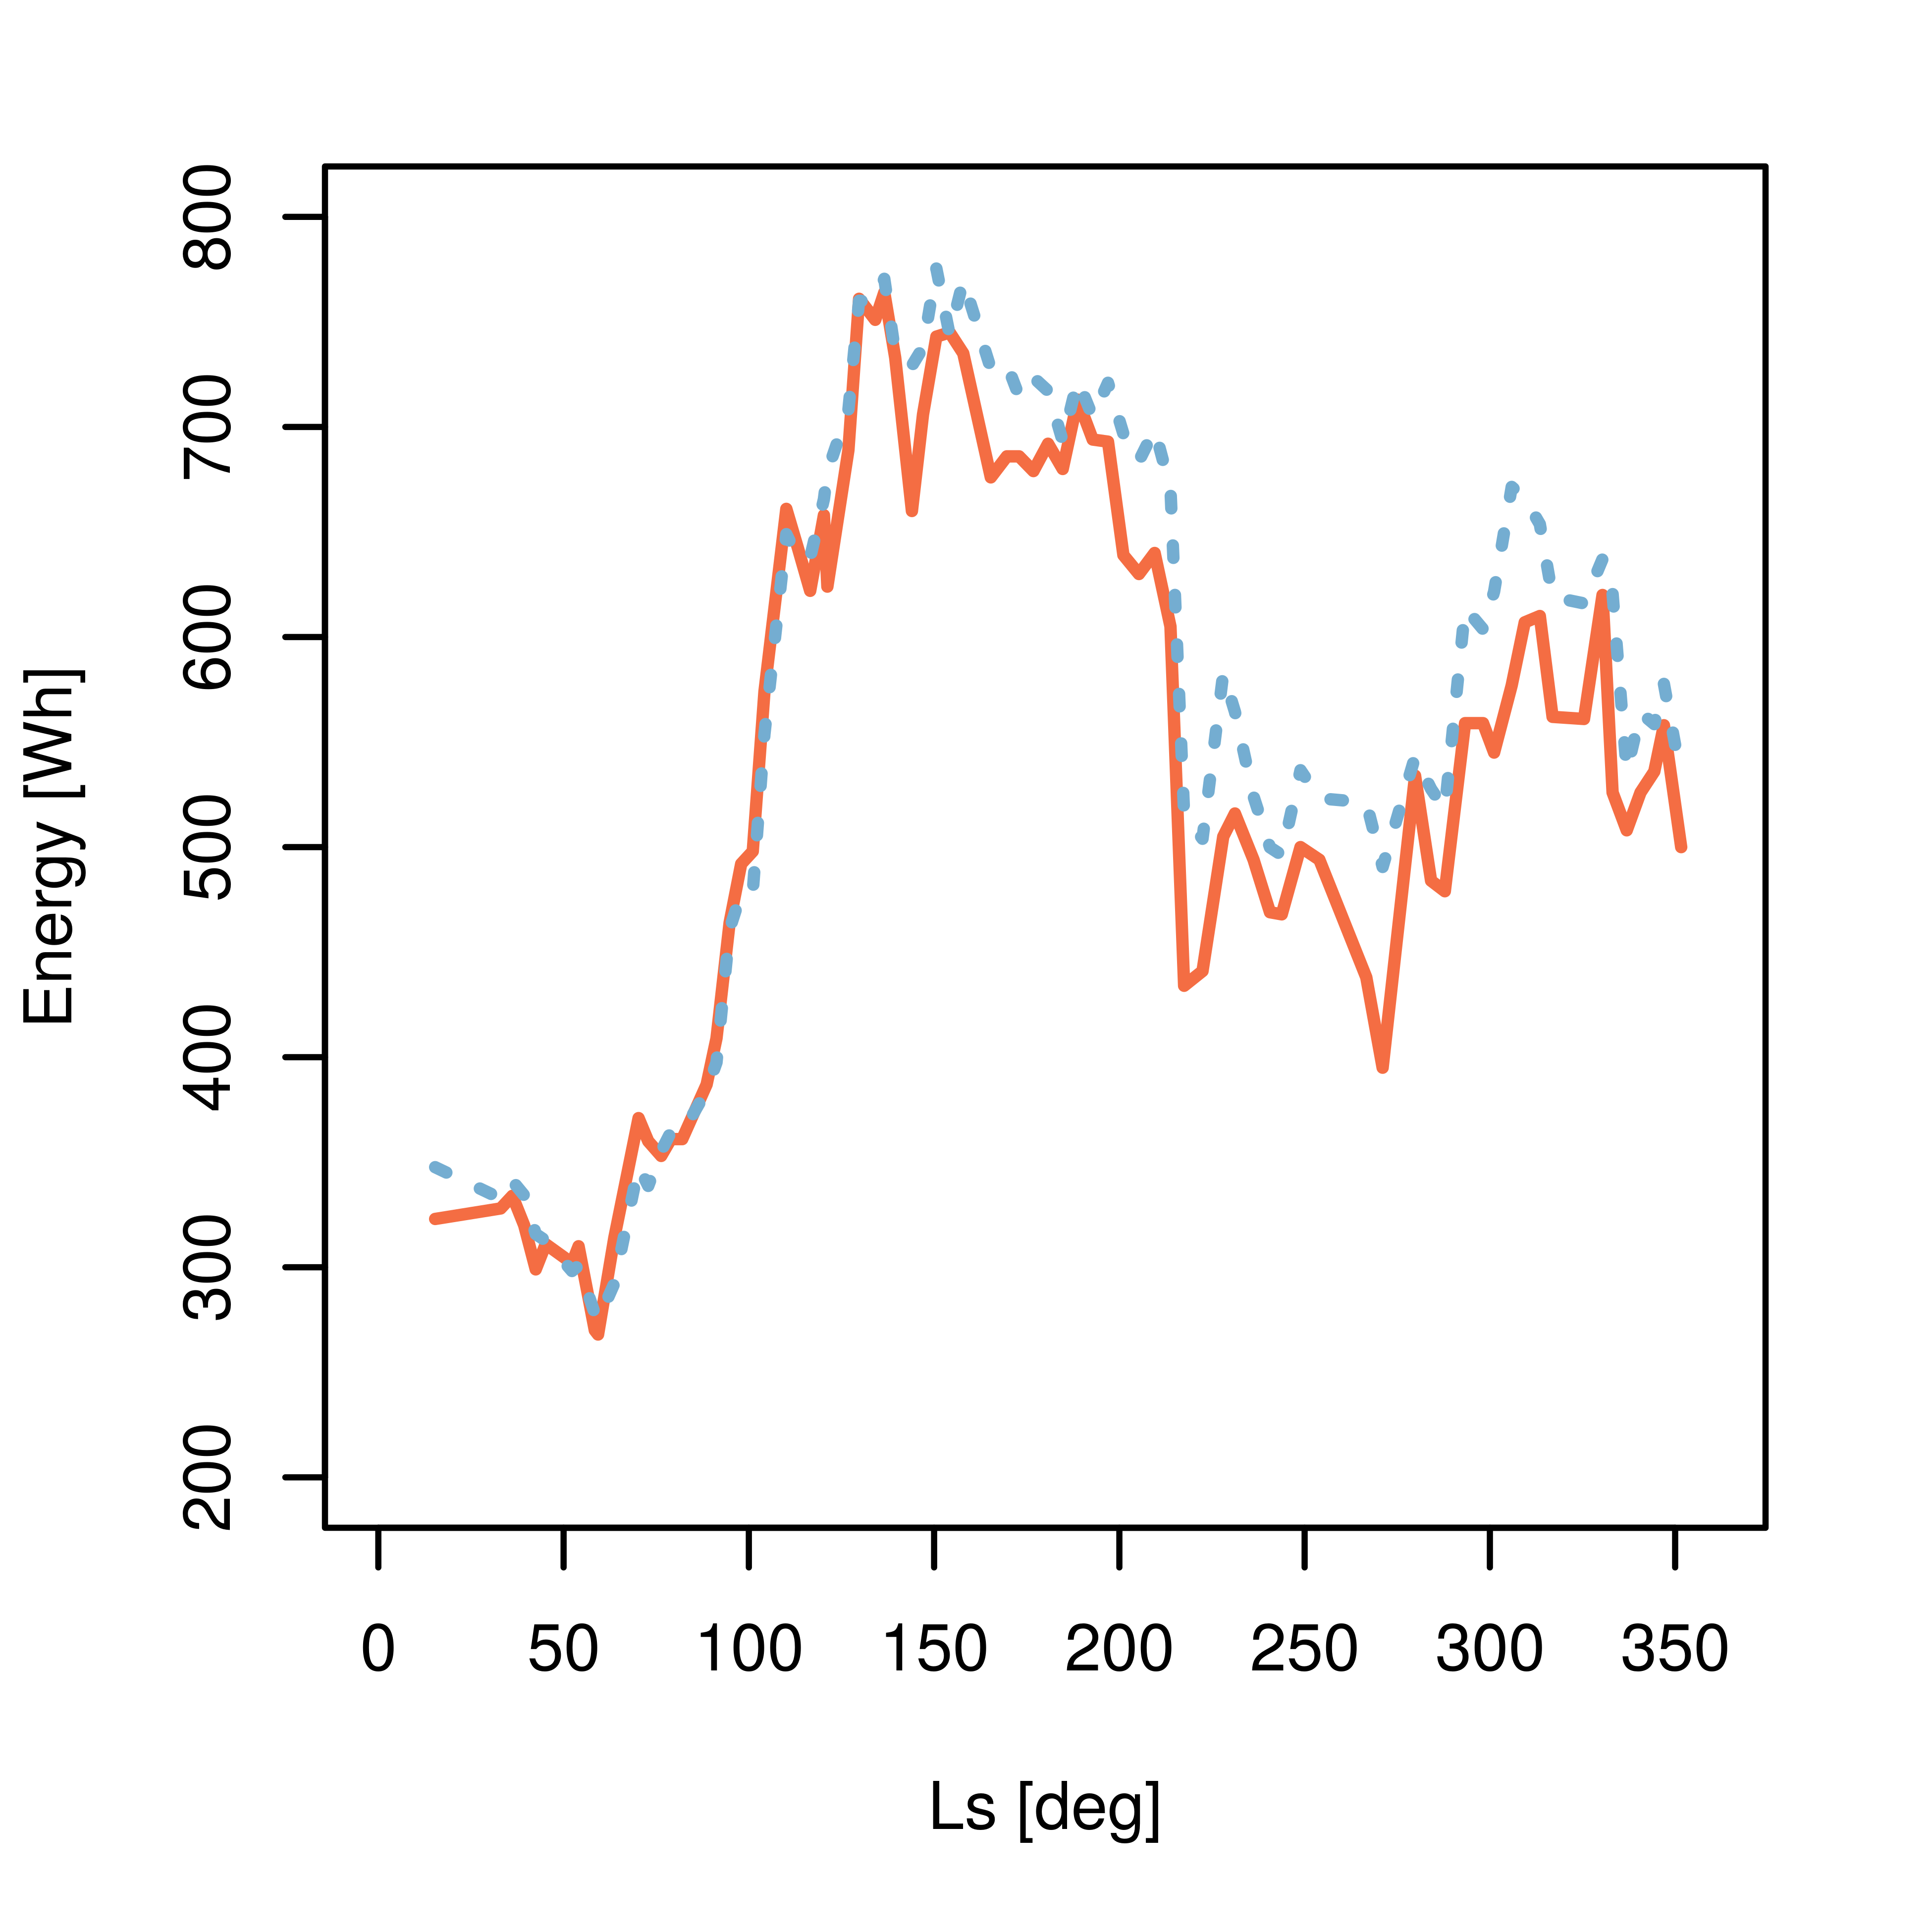
\includegraphics[height=\graphicsHeight]{sections/mars-solar-energy/photovoltaic-energy/plots/predicted-vs-measured-energy-my32.png}
  		\subcaption{MY32}
  		\label{fig:plot:sub:mer-energy-production-predicted-vs-reported-my32}
  	\end{subfigure}\hfill
	   \begin{subfigure}[t]{\subfigureWidth}
      \centering
  		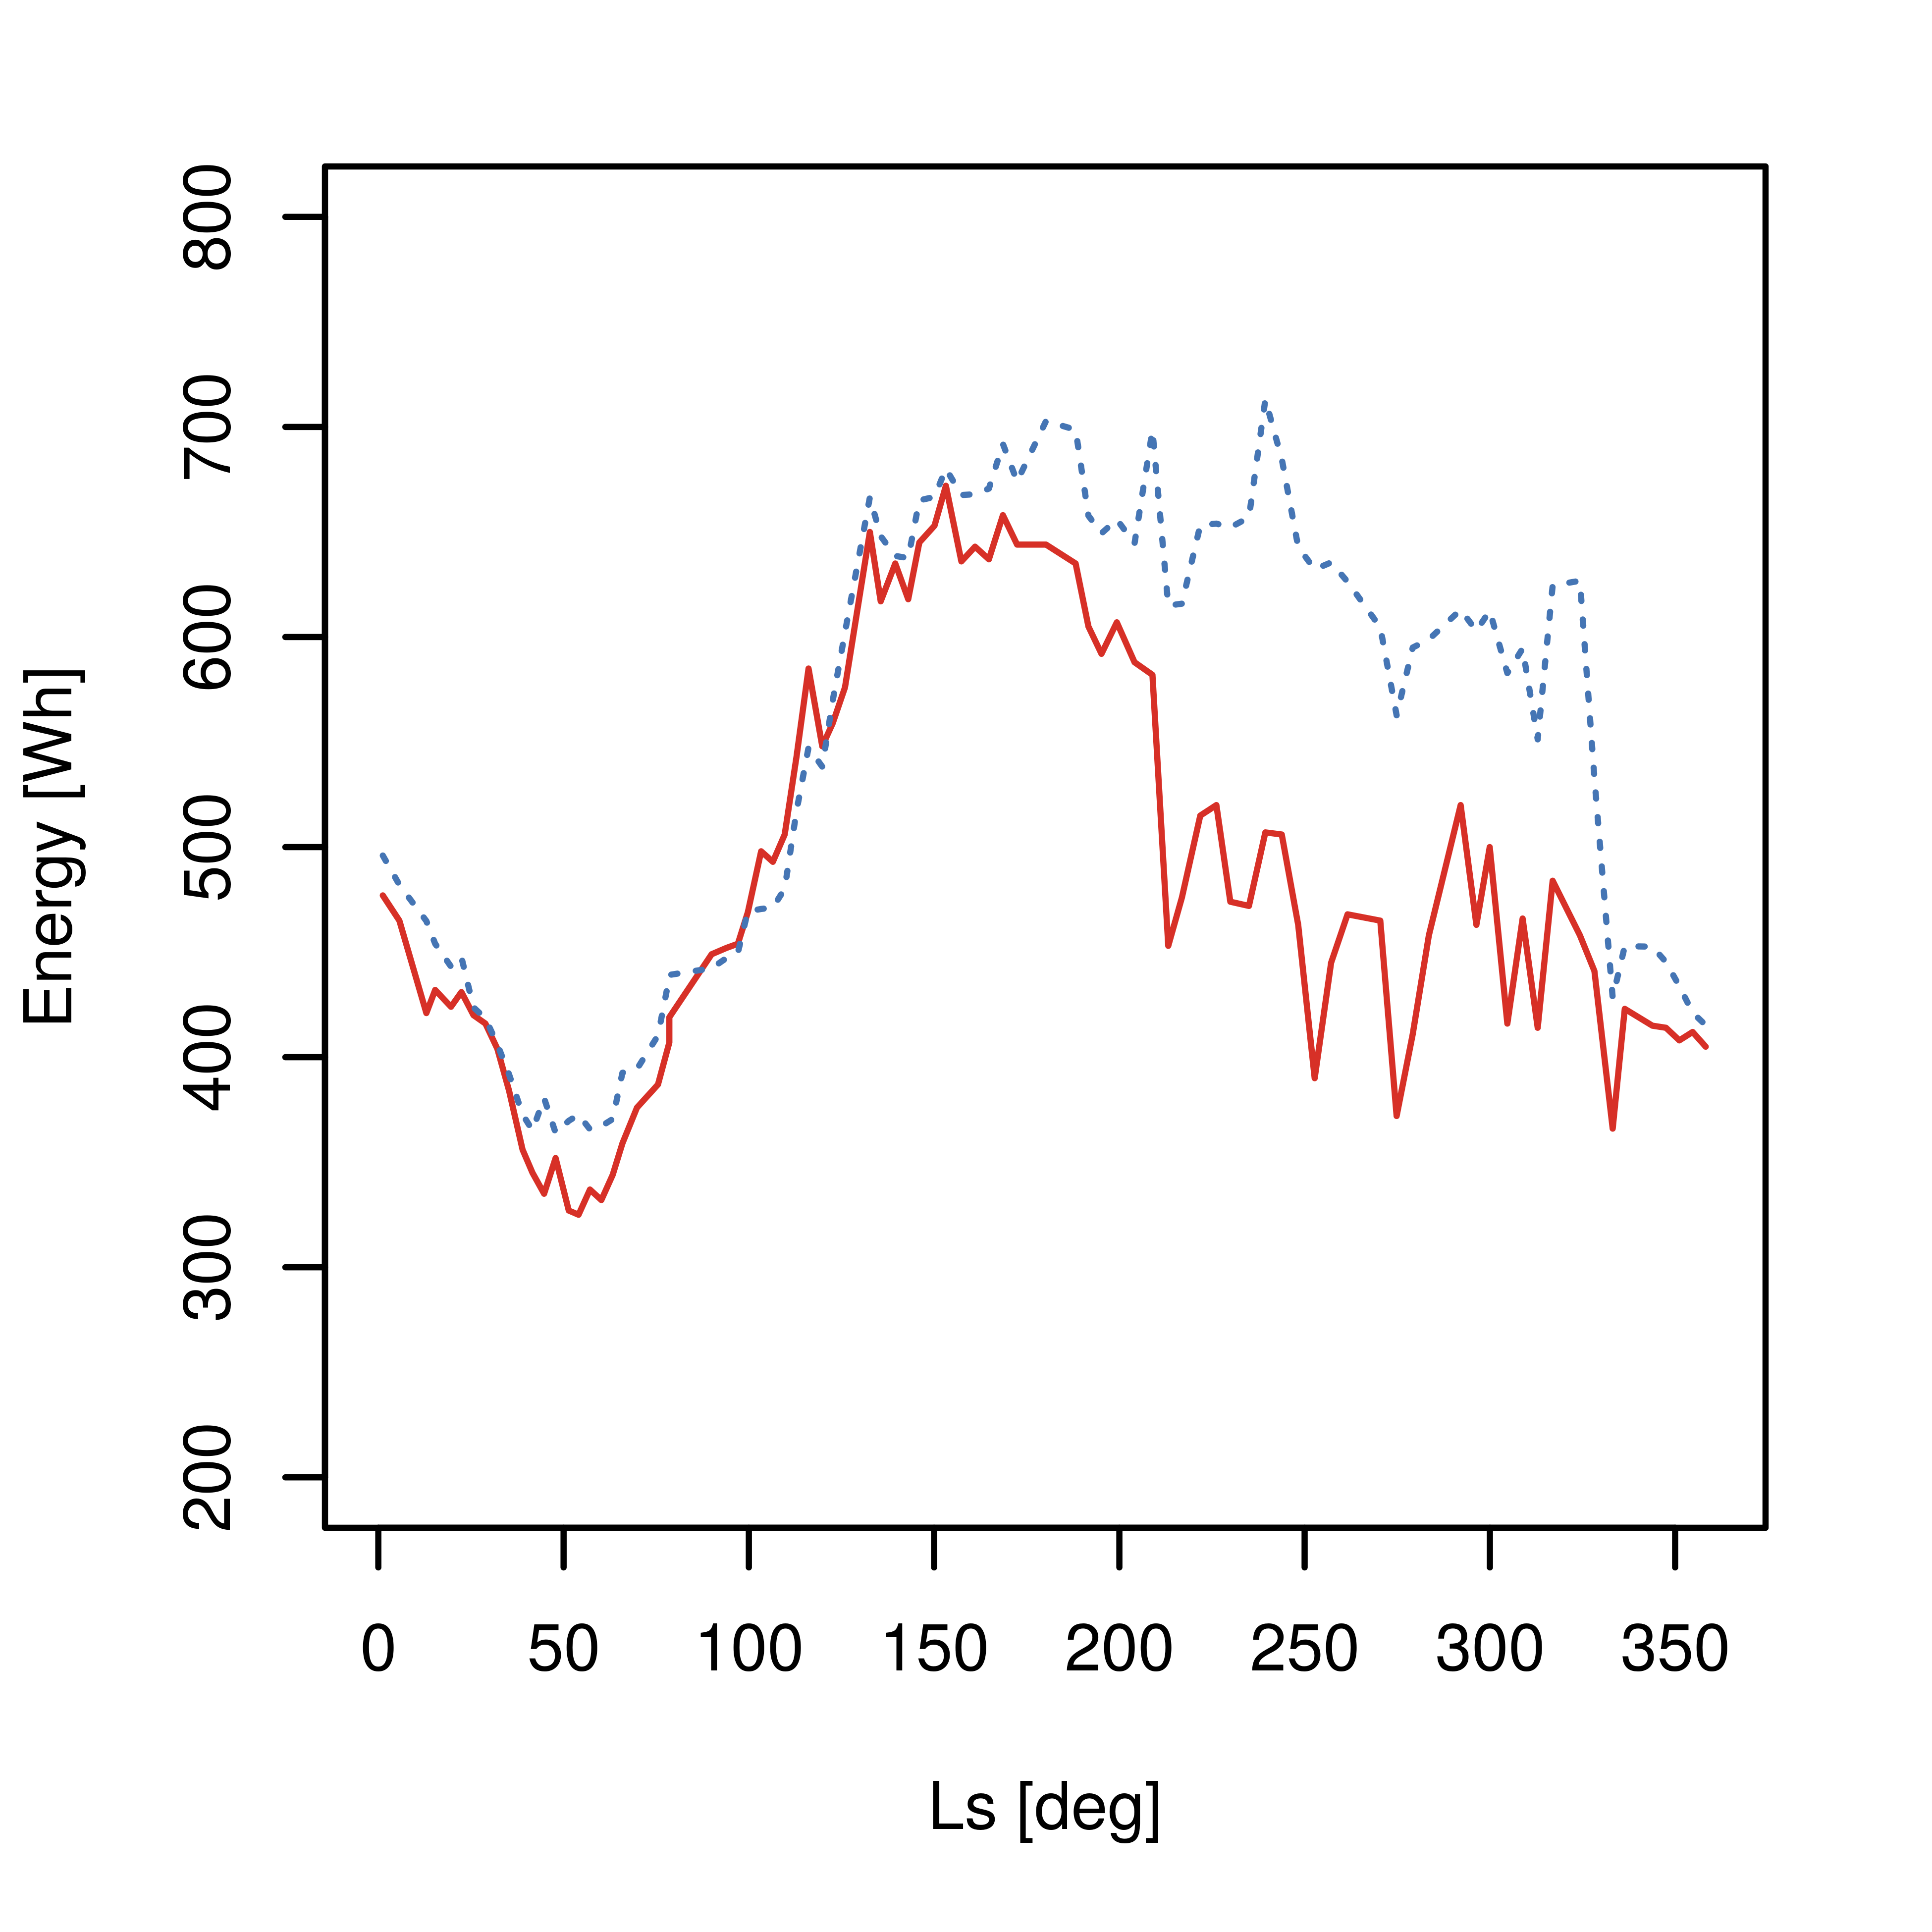
\includegraphics[height=\graphicsHeight]{sections/mars-solar-energy/photovoltaic-energy/plots/predicted-vs-measured-energy-my33.png}
  		\subcaption{MY33}
  		\label{fig:plot:sub:mer-energy-production-predicted-vs-reported-my33}
	   \end{subfigure}\hfill
    \caption[MER Opportunity PV energy production: predicted vs reported]
            {MER Opportunity PV energy production: predicted vs reported. Not shown are data for MY28 and MY34 which have also been scraped from the rover's status update logs.}
	\label{fig:plot:mer-energy-production-predicted-vs-reported}
\vspace{-2ex}
\end{figure}

\clearpage

A clear outlier is observed during the second half of MY33 in which predicted daily energy productions are much higher than what was reported. This is due to the rover's inclined descent through ``Bitterroot Valley'' during an intensive investigation into a gully at Endeavour Crater's western rim. Energy production predictions with horizontal surface Equation \ref{eq:SA_energy} not suited due to the inclination and orientation of such a descent. Applying Equation \ref{eq:SA_slope_energy} for $E_{\beta}$ would be more applicable. As such, data from MY33 is not considered in the validation exercise for horizontal surfaces.

\todo[inline]{\textbf{TODO:} Include reference to rover update for Bitterroot Valley descent.}
% Source: https://mars.nasa.gov/mer/mission/rover-status/opportunity/recent/all/?y=2016
% Source: https://www.nasa.gov/feature/jpl/rover-takes-on-steepest-slope-ever-tried-on-mars

Not included in Figure \ref{fig:plot:mer-energy-production-predicted-vs-reported} is data for MY34 during which the rover spent most of the year driving down ``Perseverance Valley'' on the west rim of Endeavour Crater. As was the case for MY33, applying Equation \ref{eq:SA_energy} for the MY34 would not be appropriate considering the rover's inclination during descents and is not considered in the validation exercise for horizontal surfaces.

% Source:https://mars.nasa.gov/mer/mission/rover-status/opportunity/recent/all/?y=2017
% Opportunity Remains at Current Location Due to Solar Conjunction
% sols 4787 to 4792, July 12, 2017 - July 17, 2017
% Opportunity entered Perseverance Valley on the west rim of Endeavour crater. The rover is positioned within the valley where she will spend the solar conjunction period.

Divergences from the predicted energy production are presented in Figure \ref{fig:plot:mer-energy-prediction-divergences} from which a -33\%/+7\% error margin range is observed. Negative values indicate predicted daily energy production greater than what was measured and the inverse is indicated by positive values.

\begin{figure}[h]
  \centering
  \hypersetup{linkcolor=captionTextColor}
  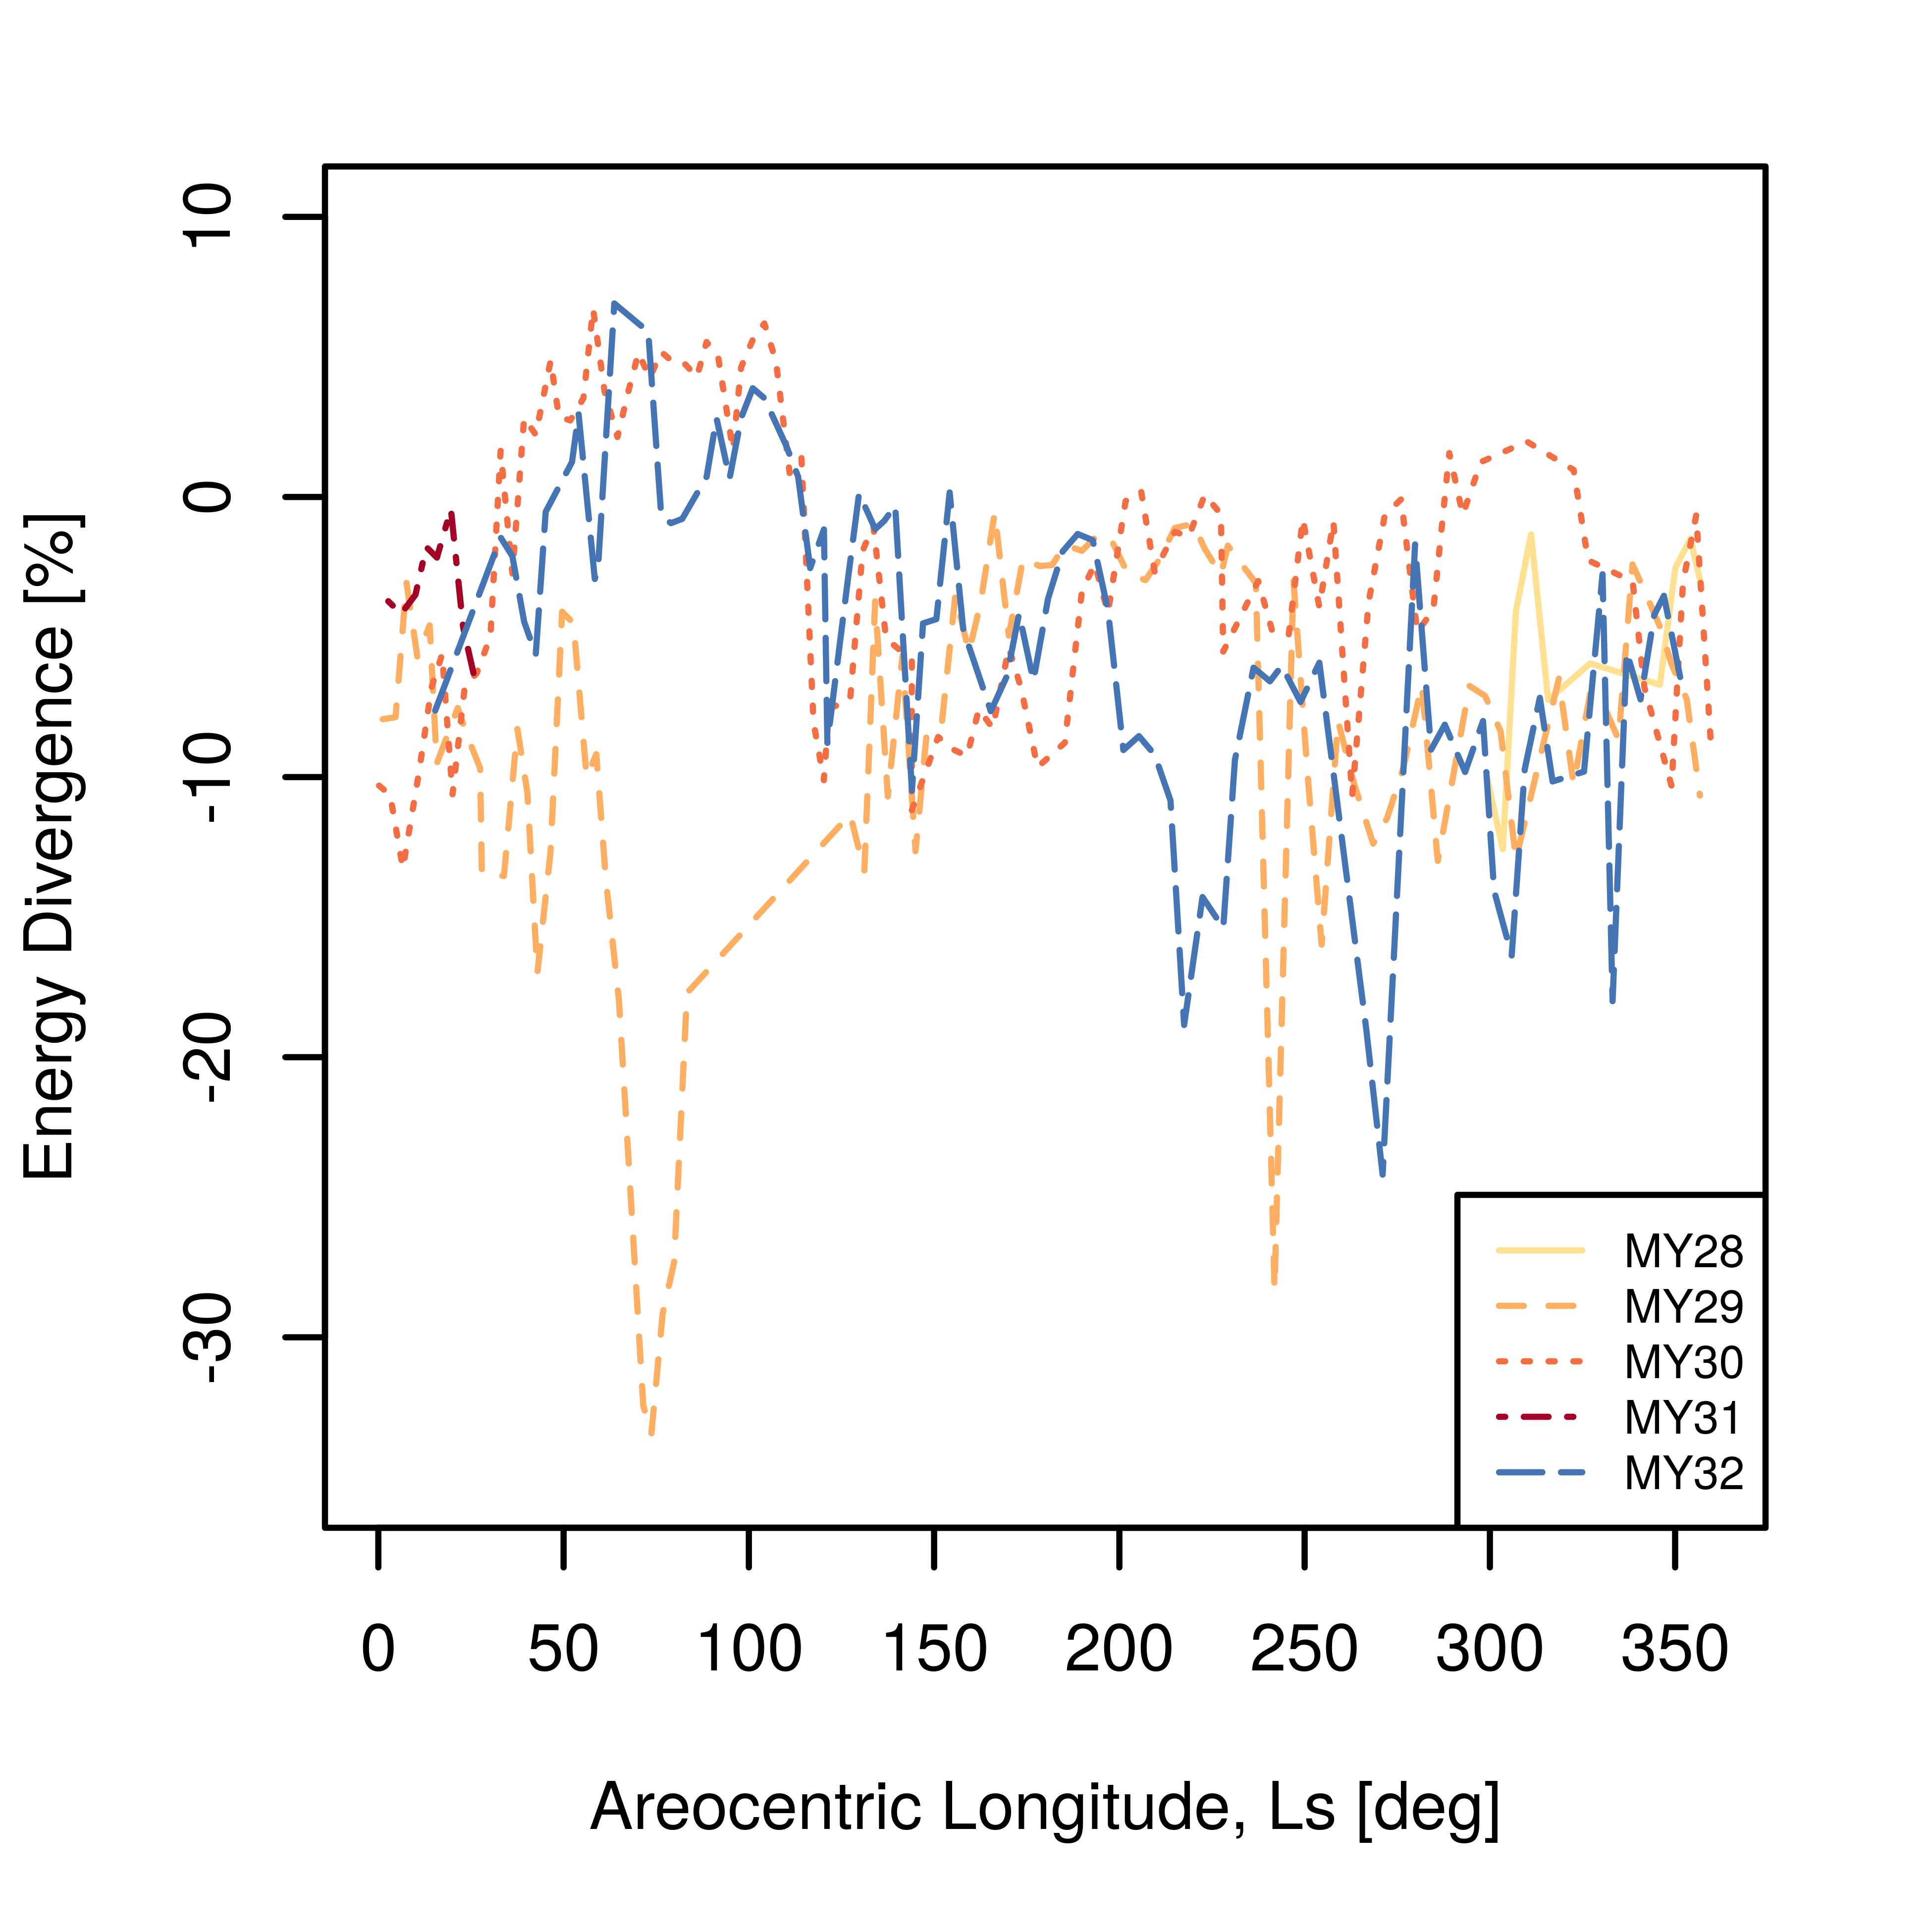
\includegraphics[width=0.5\linewidth]{sections/mars-solar-energy/photovoltaic-energy/plots/energy-prediction-divergences-from-my28-to-my32.png}\\
  \caption[Divergences from predicted \ac{MER} Opportunity \ac{PV} energy production]
          {Divergences from predicted \ac{MER} Opportunity \ac{PV} energy production.}
  \label{fig:plot:mer-energy-prediction-divergences}
\end{figure}

\clearpage

Figure \ref{fig:plot:binned-error-margins} bins the distribution of divergences across the -33\%/+7\% error margin range into 5\% increments. 65.5\% of the divergences occur within a -10\%/0\% error margin and 90.7\%  within -15\%/+5\%.

\begin{figure}[h]
  \centering
  \hypersetup{linkcolor=captionTextColor}
  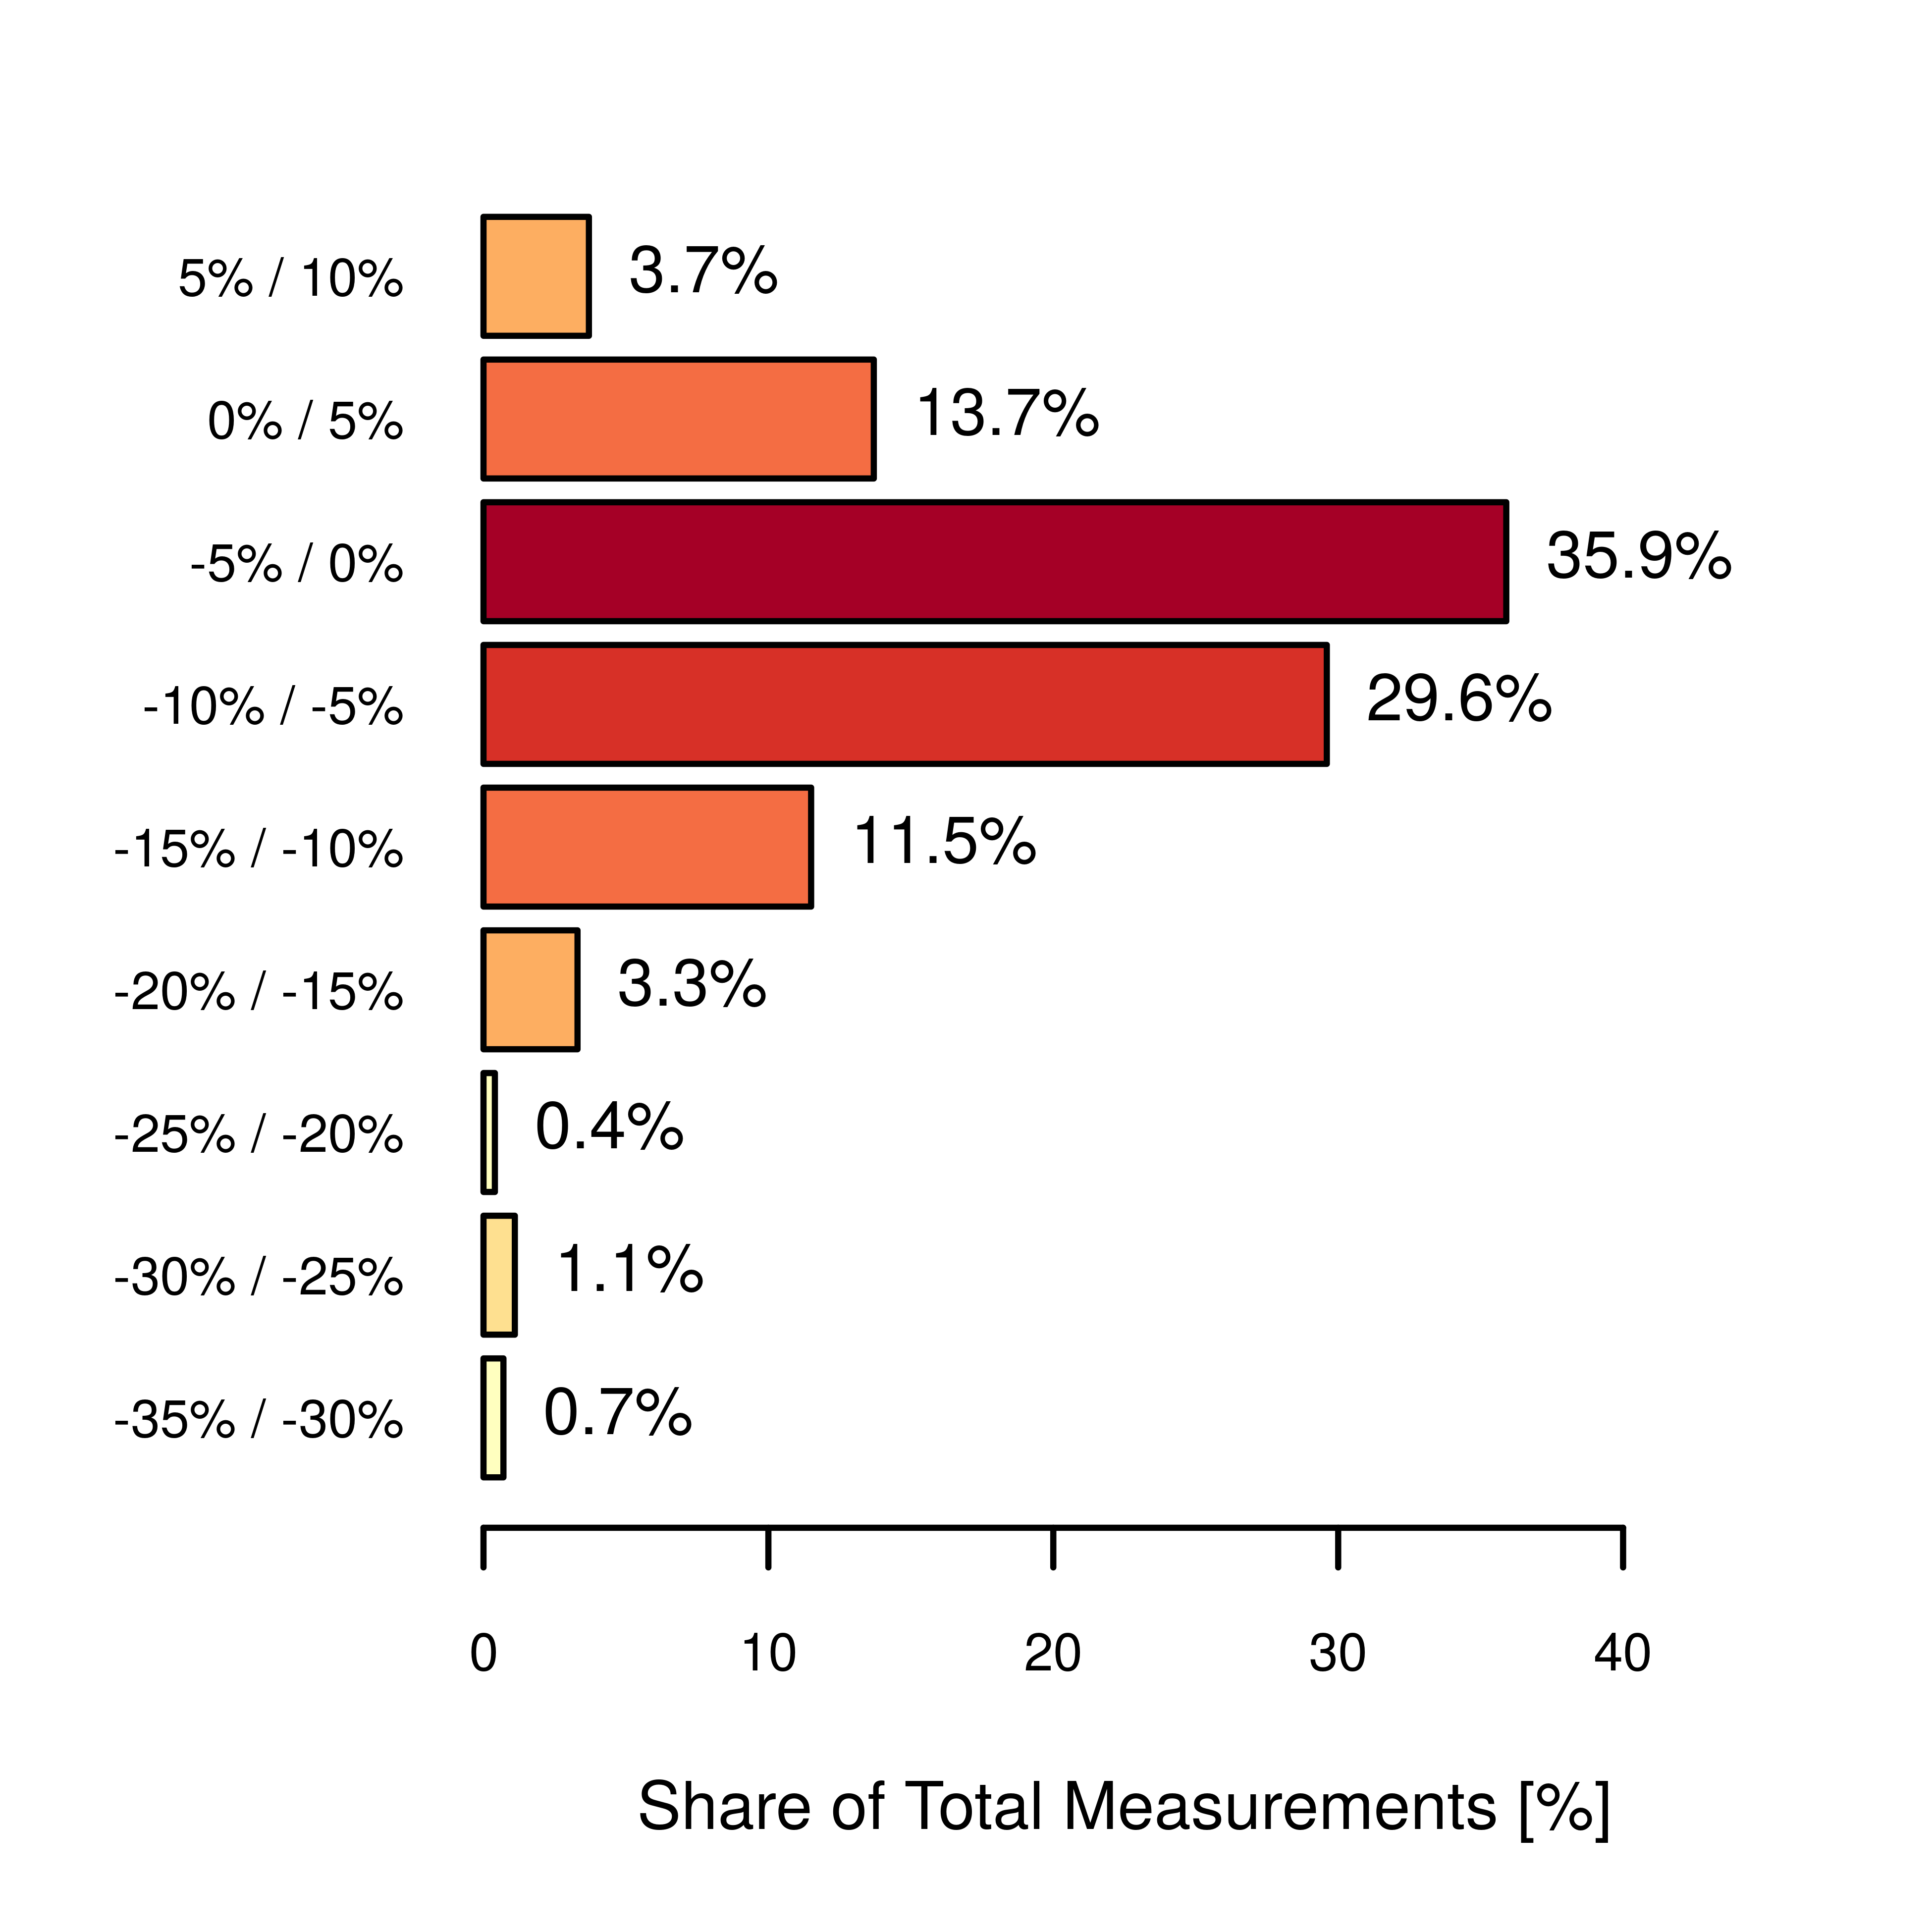
\includegraphics[width=0.5\linewidth]{sections/mars-solar-energy/photovoltaic-energy/plots/binned-error-margins.png}\\
  \caption[Binned error margins]
          {Binned error margins.}
  \label{fig:plot:binned-error-margins}
\end{figure}

The wide error margin range is thus a result of isolated local maxima outliers, notably at Sol 2204 (-33\%), 2218 (-27\%), 2519 (-28\%), and 3901 (-24\%). Table \ref{tab:divergences-less-than-m20pc} lists all divergences that are beyond -20\%.

\begin{table}[h]
    \footnotesize
    \centering
    \caption[Divergences from predicted Opportunity energy production beyond \SI{-20}{\percent}]
        {Divergences from predicted Opportunity energy production beyond \SI{-20}{\percent}.}
    \label{tab:divergences-less-than-m20pc}
    \begin{tabular}{|l|c|c|c|c|c|c|c|}
    \hline
    \multicolumn{1}{|c|}{\multirow{2}{*}{\textbf{Date}}} & \multirow{2}{*}{\textbf{MY}} & \multirow{2}{*}{\textbf{Ls}} & \multirow{2}{*}{\textbf{Sol}} & \multicolumn{4}{c|}{\textbf{Energy [Wh]}} \\ \cline{5-8}
    \multicolumn{1}{|c|}{} &  &  &  & \textbf{Predicted} & \textbf{Measured} & \textbf{Diff.} & \textbf{Diff. [\%]} \\ \hline
    1-APR-2010 & 29 & 72 & 2199 & 315 & 238 & 77 & -32 \\
    6-APR-2010 & 29 & 74 & 2204 & 314 & 235 & 79 & -33 \\
    13-APR-2010 & 29 & 77 & 2211 & 293 & 227 & 66 & -29 \\
    20-APR-2010 & 29 & 80 & 2218 & 314 & 247 & 67 & -27 \\ \hline
    23-FEB-2011 & 29 & 242 & 2519 & 539 & 420 & 119 & -28 \\ \hline
    13-JAN-2015 & 32 & 271 & 3901 & 491 & 395 & 96 & -24 \\ \hline
    \end{tabular}
\end{table}


With the exception of Sol 2199 and 2218, possible explanations for large divergences beyond -20\% were obtained from MER Opportunity's status logs [?]:

\begin{enumerate}[label=\textbf{\textcolor{BulletBlue}{(\alph*)}}]
  \item Sol 2199: No turns or inclinations reported.
  \item Sol 2204: Turn - short sharp arc turn.
  \item Sol 2211: Inclination - crossed a series of ripples.
  \item Sol 2218: No turns or inclinations reported.
  \item Sol 2519: Turn - sharp repositioning turn.
  \item Sol 3901: Inclination - descended from the summit of 'Cape Tribulation'.
\end{enumerate}

\todo[inline]{\textbf{TODO:} Source MER Opportunity status log.}
%Sources. For terrestrial year 2010: https://mars.nasa.gov/mer/mission/rover-status/opportunity/2010/

The use of fixed daily values for the certain irradiance calculation variables also contributes to the observed divergences:

\begin{enumerate}[label=\textbf{\textcolor{BulletBlue}{(\alph*)}}]
  \item A fixed $\tau$ factor does not reflect the continuous changes in atmopheric optical depth.
  \item A fixed solar array dust factor does not reflect the irregularity of dust deposition over the entirety of the solar cell coverage area.
  \item A fixed shadowing performance loss coefficient does not reflect the diurnal changes in overshadowed area. Overshadowing changes throughout the day due to the position of the sun with respect to the location of the rover's petruding instruments, notably the Pancam Mast Assembly (PMA) as well as the low-gain and high-gain antennas.
\end{enumerate}

Attempts to narrow down the error margin range by adjusting the reported dust factor as well as shadowing and other losses are described in Appendix \ref{sec:Appendix:NarrowedEnergyPredictionErrorMarginRange}. However, these attempts resulted in overly conservative energy predictions and will not be applied.

By setting aside outliers causing divergences greater than 5\% and lesser than -15\% that were obtained with only 9.2\% of the dataset, the predicted energy production obtained with Equation \ref{eq:SA_energy} become acceptable for preliminary mission scenario analysis on a horizontal surfaces.

\subsubsection{Inclined Surface}
\label{sec:PowerAndEnergyPredictions:Validation:InclinedSurface}

Equation \ref{eq:SA_slope_energy} for energy predictions on an inclined surface requires slope and rover orientation angles in order to determine $H_{\beta}$. However, these parameters are seldom reported in the \ac{MER} Opportunity status updates.

Cherry-picked energy production measurements made while \ac{MER} Opportunity's descended into and ascended out of Endaveaour crater during MY33 were used in an attempt to validate predictions made with Equation \ref{eq:SA_slope_energy}. These measurements were selected based on traverse phases that preserved consistent orientations which could be more reliable measured from the rover's Traverse Map Archive [z].

An average slope angle of 13 degrees was assumed based on the following:
\begin{itemize}
  \item On Sol 4269 and 4270, \ac{MER} Opportunity status logs reported that the rover climbed slopes close to \SI{30}{\degree} near the crest of ``Knudsen Ridge'' [a], reaching \SI{32}{\degree} on March 10, 2016 (Sol 4310) [b].
  \item An image taken in March 22, 2016 (Sol 4322), was rotated \SI{13.5}{\degree} degrees to adjust for the tilt of the rover.
  \item Perseverance Valley extends downhill at around \SI{15}{\degree} for about 200 meters toward Endeavour crater's interior [c].
\end{itemize}

As was the case in Section \ref{sec:PowerAndEnergyPredictions:Validation:HorizontalSurface}, performance ratios described in Section \ref{sec:PowerAndEnergyPredictions:PerformanceRatio} were also used. Due to large uncertainties regarding slope rover orientation angles, this section only aims to validate that using Equation \ref{eq:SA_slope_energy} results in smaller energy predictions divergences than what would otherwise be obtained using Equation \ref{eq:SA_energy}. The results are presented in Table \ref{tab:divergences-inclined-surfaces}:

\begin{table}[h]
\footnotesize
\centering
\caption{Divergences from predicted MER Opportunity PV energy production on inclined surfaces.}
\label{tab:divergences-inclined-surfaces}
\begin{tabular}{|c|c|c|c|c|c|}
\hline
\multicolumn{1}{|l|}{\multirow{3}{*}{\textbf{Sol}}} & \multirow{3}{*}{\textbf{\begin{tabular}[c]{@{}c@{}}Measured\\ Energy\\ {[}Wh{]}\end{tabular}}} & \multicolumn{4}{c|}{\textbf{Predicted Energy}} \\ \cline{3-6}
\multicolumn{1}{|l|}{} &  & \multicolumn{2}{c|}{\textbf{Horizontal Surface}} & \multicolumn{2}{c|}{\textbf{Inclined Surface}} \\ \cline{3-6}
\multicolumn{1}{|l|}{} &  & \multicolumn{1}{l|}{\textbf{$E$ {[}Wh{]}}} & \multicolumn{1}{l|}{\textbf{Diff. {[}\%{]}}} & \multicolumn{1}{l|}{\textbf{$E_{\beta}$ {[}Wh{]}}} & \multicolumn{1}{l|}{\textbf{Diff. {[}\%{]}}} \\ \hline
4493 & 515 & 653 & -27 & 407 & 21 \\ \hline
4582 & 411 & 595 & -45 & 535 & -30 \\ \hline
4623 & 416 & 583 & -40 & 284 & 32 \\ \hline
4630 & 466 & 595 & -28 & 526 & 13 \\ \hline
\end{tabular}
\end{table}


Equation \ref{eq:SA_slope_energy} resulted in a larger divergence range than with Equation \ref{eq:SA_energy} at -30\%/32\% for the former and -45\%/-27\% for the latter. However, the magnitude of divergences are smaller with Equation \ref{eq:SA_slope_energy}. Furthermore, with the exception of Sol 4582, divergences with \ref{eq:SA_slope_energy} result in conservative under-estimated energy predictions rather than the worst-case over-estimated values consistently obtained with Equation \ref{eq:SA_energy}.

The pool of measured data used for this validation was much too small to draw convincing conclusions and the magnitude of divergences remained significantly large. Inaccurate slope and rover orientation angles are likely to have contributed to unfavourable results. Further data will have to be obtained to validate Equation \ref{eq:SA_slope_energy} against reported measurements. However, for the purpose of this thesis, mission scenario analysis on inclined surfaces will still rely on predictions obtained with Equation \ref{eq:SA_slope_energy} in light of it being derived from applying solar geometry to Equation \ref{eq:SA_energy}, with which favourably results were obtained as described in Section \ref{sec:PowerAndEnergyPredictions:Validation:HorizontalSurface}.

% [z] Rover traverse map. [https://mars.nasa.gov/mer/mission/traverse-maps/opportunity/]
% [a] https://mars.nasa.gov/mer/mission/rover-status/opportunity/recent/all/?y=2016
% [b] https://www.jpl.nasa.gov/news/news.php?feature=6193
% [c] https://www.planetary.org/explore/space-topics/space-missions/mer-updates/2018/04-mer-update-special-perseverance-valley-lpsc-2018.html

%Particularly while it was exploring steep outcrops within 'Marathon Valley' when the rover was inclined on the slopes of 'Knudsen Ridge' at Sol 4303 (March 1, 2016).
%The rover's tilt hit 32 degrees on March 10 while Opportunity was making its closest approach to an intended target near the crest of "Knudsen Ridge."

\subsection{Summary}
\todo[inline]{\textbf{TODO:} Write section summary.}


\clearpage
\section{Mission Sites}
\label{sec:MarsSolarEnergy:MissionSites}
The missions sites at Iani Chaos and Ismenius are selected as a prerequisite to determine environmental constraints pertaining to available solar radiation on the Martian surface.

\subsection{Selection Criteria}
\label{sec:MissionSites:SelectionCriteria}
The mission site selection criteria are:

\begin{enumerate}[label=\textbf{\textcolor{BulletBlue}{(\alph*)}}]
    \item The location is of scientific interest, supported by past or ongoing research.
    \item The terrain features complex morphologies so that scenarios with inclined solar array surfaces may be simulated from which the rover's active suspension system may also be evaluated.
    \item Landing sites for the location have been proposed in preceedings such as with the \ac{MSL} Landing Site Workshops in \citeother{MSLLandingSites}. Such proposals suggest technical feasibility in landing a rover for the proposed locations.
    \item \ac{HiRISE} \ac{DTM} are available near the \ac{ROI} so that 3D environment models may be loaded on the mission simulation platform.
    \item The planetary latitude is close to that of the \ac{MER} Opportuniy mission in order to enable future comparative analysis of simulation results with 14 years worth of \ac{MER} power budget data. This target planetary latitude is approximately \SI{2}{\degree}S.
    \item The planetary latitude is close to that of the \ac{VL1} and \ac{VL2} missions in order to more closely align with the environment conditions from which the power and energy prediction models were built. This target planetary latitude is between \SI{22}{\degree}N and \SI{48}{\degree}N.
\end{enumerate}

Conducting mission scenario simulations for both locations also ensures that a wider range of seasonal driven solar radiation variations are explored with respect to differences in planetary latitude. Iani Choas is located in the Sourthern hemisphere, close to the equator, whereas Ismenius Cavus is located in the Norhern hemispheres at a significant distance from the equator.

\subsection{Iani Chaos}
\label{sec:MissionSites:IaniChaos}
Iani Chaos is centered at approximately \SI{17}{\degree}W, \SI{2}{\degree}S, it is scientific interest due its long-lived, but likely episodic, fluvial activity \citeother{Warner2011}. In particular, hematite- and sulfite-rich light-toned layered deposits suggest past shallow water and groundwater depositional environment \citeother{Glotch2007}. \refFig{fig:mission-site-iani-chaos} shows the distribution of these deposits in region covering \SI{9}{\degree}S – \SI{4}{\degree}N latitude and \SI{12}{\degree} – \SI{32}{\degree}W longitude. Furthermore, ``topography, the observed geomorphology, and measured fracture patterns suggest that the interchaos basins formed as a result of subsurface volume loss and collapse of the crust, likely owing to effusion of groundwater to the surface'' \citeother{Warner2011}. Iani Chaos is a ``clear link to the past presence of surface and subsurface water, making the site of prime astro-biological interest.'' \citeother{Glotch2006}

\begin{figure}[h]
  \centering
  \hypersetup{linkcolor=captionTextColor}
  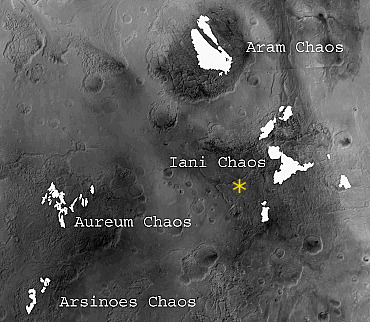
\includegraphics[width=0.7\linewidth]{sections/mars-solar-energy/mission-sites/images/iani-chaos-deposits.png}\\
  \caption[Map of light‐toned deposits in chaotic terrains in Margaritifer Terra overlaid on a \ac{MOC} \ac{WA} mosaic]
          {Map of light‐toned deposits in chaotic terrains in Margaritifer Terra overlaid on a \ac{MOC} \ac{WA} mosaic. The mapped region covers \SI{9}{\degree}S – \SI{4}{\degree}N latitude and \SI{12}{\degree} – \SI{32}{\degree}W longitude. Taken from \citeother{Glotch2007}. The yellow asterisk indicates the \ac{HiRISE} \ac{DTM} location in Western Iani Chaos which was used for mission scenario simulation.}
  \label{fig:mission-site-iani-chaos}
\end{figure}


Iani Chaos is ``among the most geomorphologically complex chaotic terrains.'' From  \citeother{Warner2011}, its morphology has been defined by:

\begin{enumerate}[label=\textbf{\textcolor{BulletBlue}{(\alph*)}}]
    \item Multiple, 1 to \SI{2}{\kilo\meter} deep basins.
    \item Flat‐topped, fractured plateaus that are remnants of highland terrain.
    \item Knobby, fractured remnants of highland terrain.
    \item Plateaus with a knobby surface morphology.
    \item Interchaos grooved terrain.
    \item \ac{ILD}.
    \item Mantling material.
\end{enumerate}

\clearpage
\refFig{fig:sub:western-iani-chaos-dtm} shows a section of the \ac{DTM} of Western Iani Chaos which was loaded on the rover's mission simulation plaform. The topography of the area is shown in \refFig{fig:sub:western-iani-chaos-dtm-altimetry}.


\begin{figure}[h]
\captionsetup[subfigure]{justification=centering}
%\vspace{-2ex}
	\centering
    %% setup sizes
    \setlength{\subfigureWidth}{0.50\textwidth}
    \setlength{\graphicsHeight}{120mm}
    %% kill hyper-link highlighting
    \hypersetup{hidelinks=true}%
    %% the figures
    \begin{subfigure}[t]{\subfigureWidth}
        \centering
        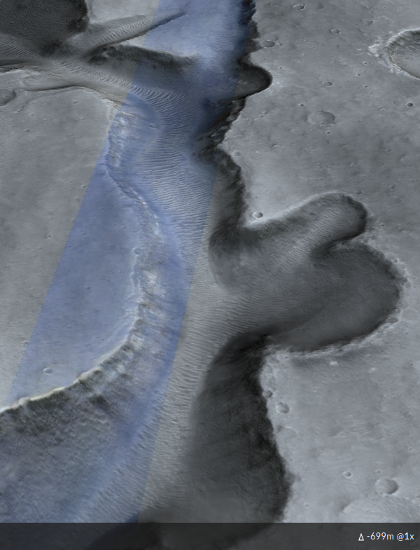
\includegraphics[height=\graphicsHeight]{sections/mars-solar-energy/mission-sites/images/western-iani-chaos-dtm.png}
        \subcaption{\ac{DTM}}
        \label{fig:sub:western-iani-chaos-dtm}
    \end{subfigure}\hfill
    \begin{subfigure}[t]{\subfigureWidth}
        \centering
        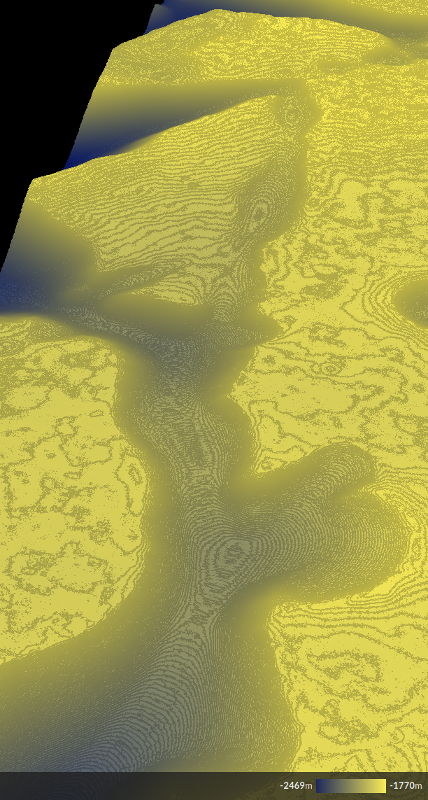
\includegraphics[height=\graphicsHeight]{sections/mars-solar-energy/mission-sites/images/western-iani-chaos-dtm-altimetry.png}
  		\subcaption{Topography}
		\label{fig:sub:western-iani-chaos-dtm-altimetry}
	\end{subfigure}\\[0.8ex]
    \caption[Western Iani Chaos \ac{HiRISE} \ac{DTM}]
            {Western Iani Chaos \ac{HiRISE} \ac{DTM}. Taken from \citeother{AreoBrowser}. Image: \ac{NASA}/\ac{JPL}/University of Arizona.}
    \label{fig:western-iani-chaos}
\vspace{-2ex}
\end{figure}

\clearpage
\subsection{Ismenius Cavus}
\label{sec:MissionSites:IsmeniusCavus}
Ismenius Cavus is located at \SI{33.5}{\degree}N, \SI{17}{\degree}E, with elevations ranging from \SI{-3.5}{\kilo\meter} and \SI{-1.5}{\kilo\meter}. It is a basin where several fluvial valleys converge and is located ``at the junction between current mid-latitude ice deposits and low latitude clay minerals'', hosting science and resource regions of interest ``with both present ice and past lake sediments with clay minerals'' \citeother{Dehouck2010} \citeother{Dehouck2015}. Geologic context for this mission site area is provided with \refFig{fig:mission-site-ismenius-cavus}.

\begin{figure}[h]
  \centering
  \hypersetup{linkcolor=captionTextColor}
  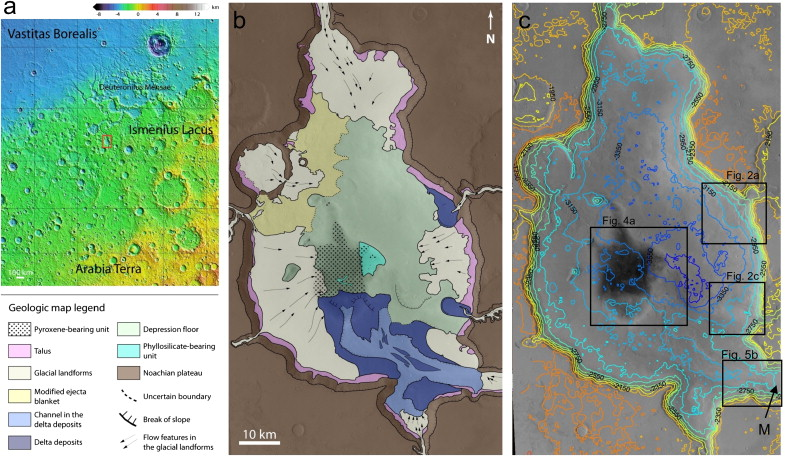
\includegraphics[width=0.8\linewidth]{sections/mars-solar-energy/mission-sites/images/ismenius-cavus.png}\\
  \caption[Geologic context for Ismenius Cavus mission site area]
          {Geologic context of the mission site area, taken from \citeother{Dehouck2010}. Location shown on a \ac{MOLA} reference map (a) and a geologic map of Ismenius Cavus (b). The yellow asterisk indicates the \ac{HiRISE} \ac{DTM} location which was used for mission scenario simulation.}
  \label{fig:mission-site-ismenius-cavus}
\end{figure}

% https://www.uahirise.org/dtm/dtm.php?ID=ESP_052945_2150

Supported science of interest are taken from \citeother{Dehouck2015}:
\begin{enumerate}[label=\textbf{\textcolor{BulletBlue}{(\alph*)}}]
    \item Potential for past habitability.
    \item Potential for organic matter with surface exposure.
    \item Noachian/Hesperian rocks with trapped atmospheric gases.
    \item High likelohood of surface-atmosphere exchange.
    \item Amazonian subsurface or high-latitude ice or sediment.
    \item Range of martian geologic time; datable surfaces.
    \item Evidence of aqueous processes.
    \item Potential for interpreting relative ages.
    \item Near-surface ice, glacial or permafrost.
    \item Noachian or pre-Noachian bedrock units.
    \item Diversity of aeolian sediments and/or landforms.
\end{enumerate}

Supported resources of interest are also presented in \citeother{Dehouck2015} with clay minerals and water ice being two main resources for water. Furthermore, there is a potential for metal/silicon. These resources are located no more than \SI{3}{\meter} below the surface. Mobile material resources for construction purposes also exist.

\refFig{fig:sub:ismenius-cavus-dtm} shows a section of the \ac{DTM} which was loaded on the rover's mission simulation plaform. It features an exit breach in a well-preserved crater. The topography of the area is shown in \refFig{fig:sub:western-iani-chaos-dtm-altimetry}.
\vspace{0.5cm}

\begin{figure}[h]
\captionsetup[subfigure]{justification=centering}
\vspace{-2ex}
	\centering
    %% setup sizes
    \setlength{\subfigureWidth}{0.50\textwidth}
    \setlength{\graphicsHeight}{100mm}
    %% kill hyper-link highlighting
    \hypersetup{hidelinks=true}%
    %% the figures
    \begin{subfigure}[t]{\subfigureWidth}
        \centering
        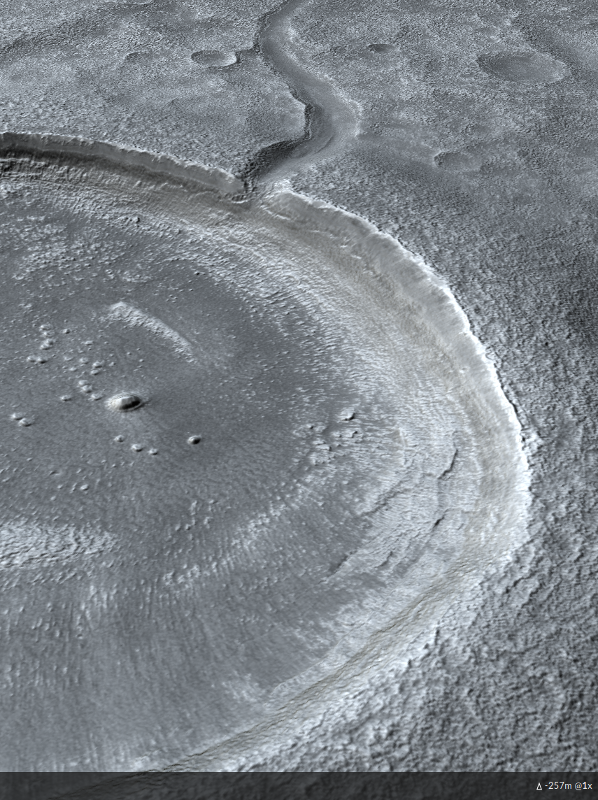
\includegraphics[height=\graphicsHeight]{sections/mars-solar-energy/mission-sites/images/ismenius-cavus-dtm.png}
        \subcaption{\ac{DTM}}
        \label{fig:sub:ismenius-cavus-dtm}
    \end{subfigure}\hfill
    \begin{subfigure}[t]{\subfigureWidth}
        \centering
        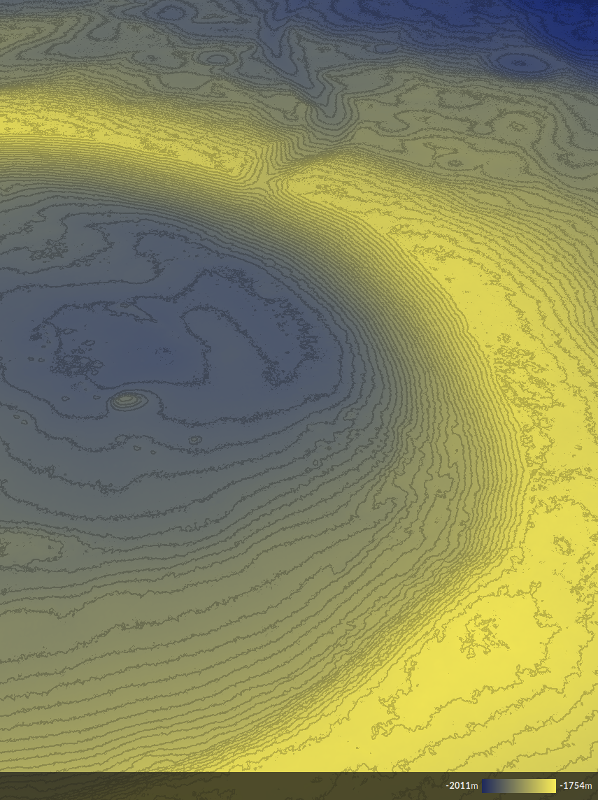
\includegraphics[height=\graphicsHeight]{sections/mars-solar-energy/mission-sites/images/ismenius-cavus-dtm-altimetry.png}
  		\subcaption{Topography}
		\label{fig:sub:ismenius-cavus-dtm-altimetry}
	\end{subfigure}\\[0.8ex]
    \caption[Ismenius Cavus \ac{HiRISE} \ac{DTM}]
            {Ismenius Cavus \ac{HiRISE} \ac{DTM}, taken from \citeother{AreoBrowser}. Image: \ac{NASA}/\ac{JPL}/University of Arizona.}
    \label{fig:ismenius-cavus}
\vspace{-2ex}
\end{figure}

\clearpage
\subsection{Daily Insolation}
Worst and best case daily insolations presented in this section are considered when sizing the rover's \ac{SA}. Optical depth is typically around $\tau = 0.4$ on clear days \citemarsenv{Smith2019} and $\tau = 1–1.5$ during local dust storms \citemarsenv{Lemmon2015}. Daily insolations $\tau > 1.5$ were only considered for global dust storm season ($\SI{180}{\degree} < L_{s} < \SI{360}{\degree}$). Year long daily insolations for $\tau = 0.4$ at both sites are shown in \refFig{fig:plot:solar-insolations-for-different-beta} where optimal combinations of $\beta$ inclination and $\gamma_c$ orientation angles were used for the \ac{SA} surface. Details on these optimal angles are found in Appendix \ref{sec:Appendix:OptimalAngles}.

\begin{figure}[h]
\vspace{-2ex}
\centering
    %% setup sizes
    \setlength{\subfigureWidth}{0.50\textwidth}
    \setlength{\graphicsHeight}{60mm}
    %% kill hyper-link highlighting
    \hypersetup{hidelinks=true}%
    %% the figures
    \begin{subfigure}[t]{\subfigureWidth}
        \centering
            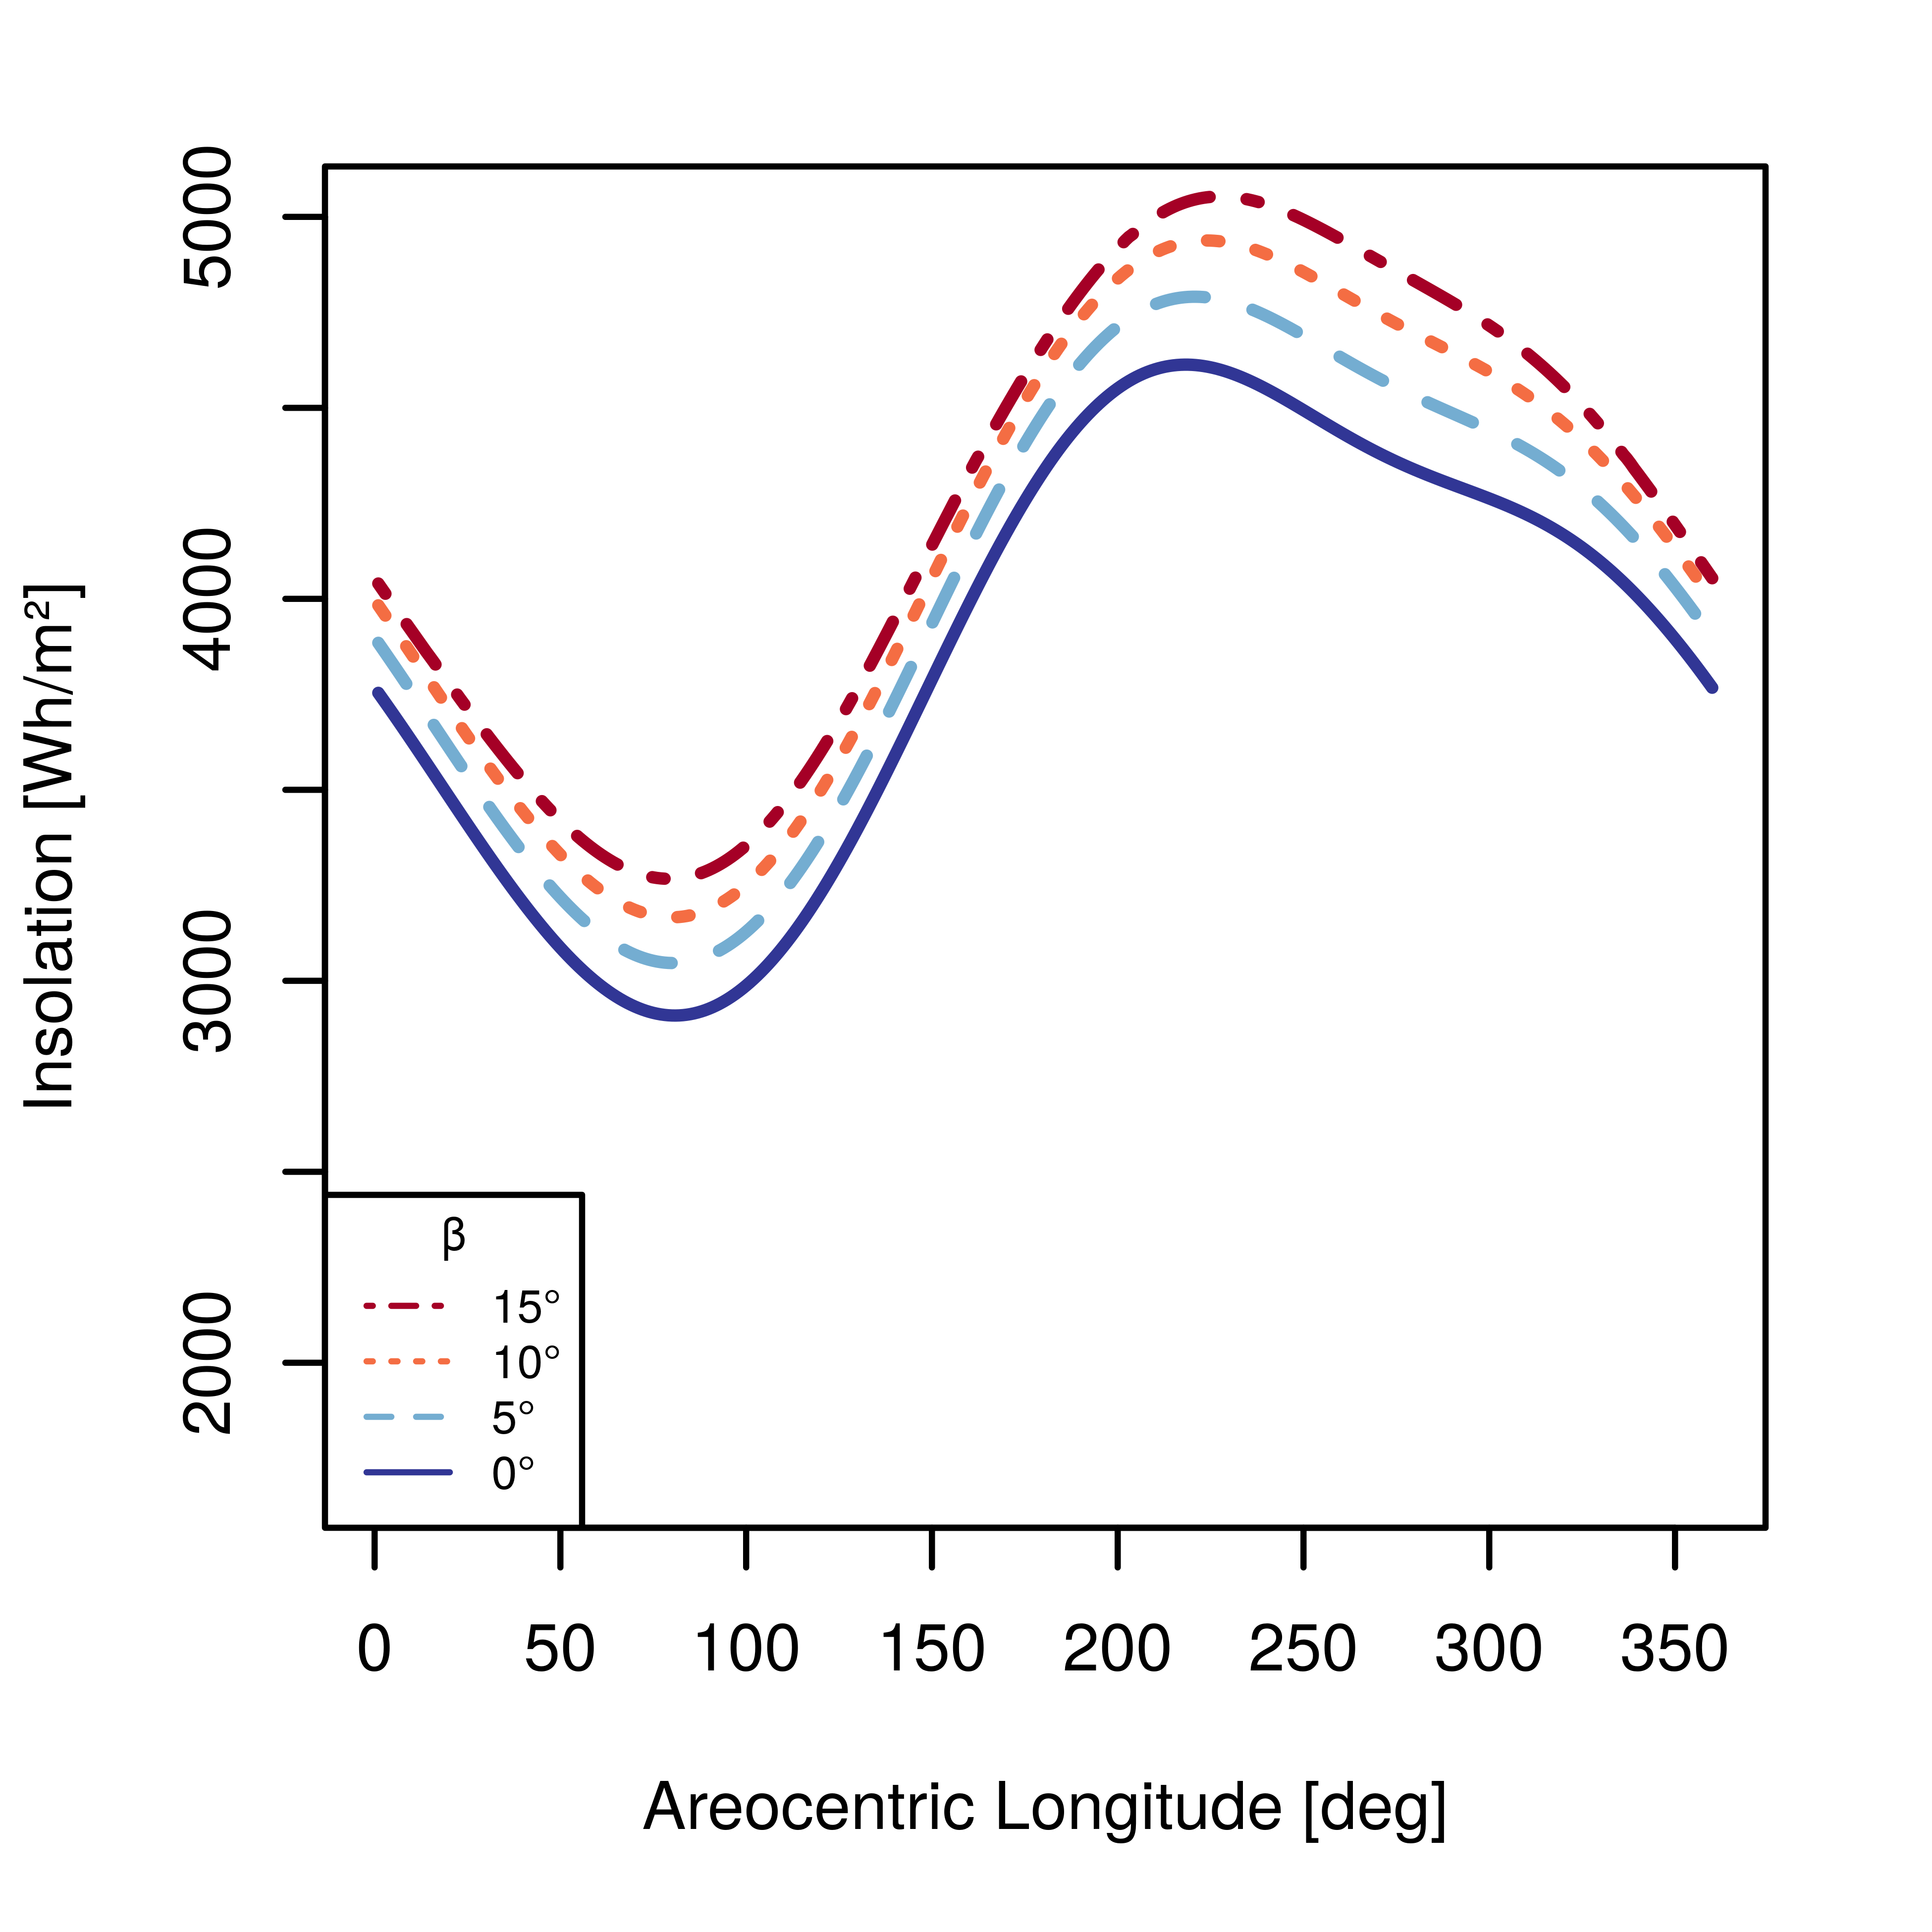
\includegraphics[height=\graphicsHeight]{sections/mars-solar-energy/mission-sites/plots/iani-chaos-solar-insolations-for-different-beta-inclinations.png}
            \subcaption{Iani Chaos.}
            \label{fig:plot:sub:solar-insolations-for-different-beta-iani-chaos}
    \end{subfigure}\hfill
    \begin{subfigure}[t]{\subfigureWidth}
        \centering
            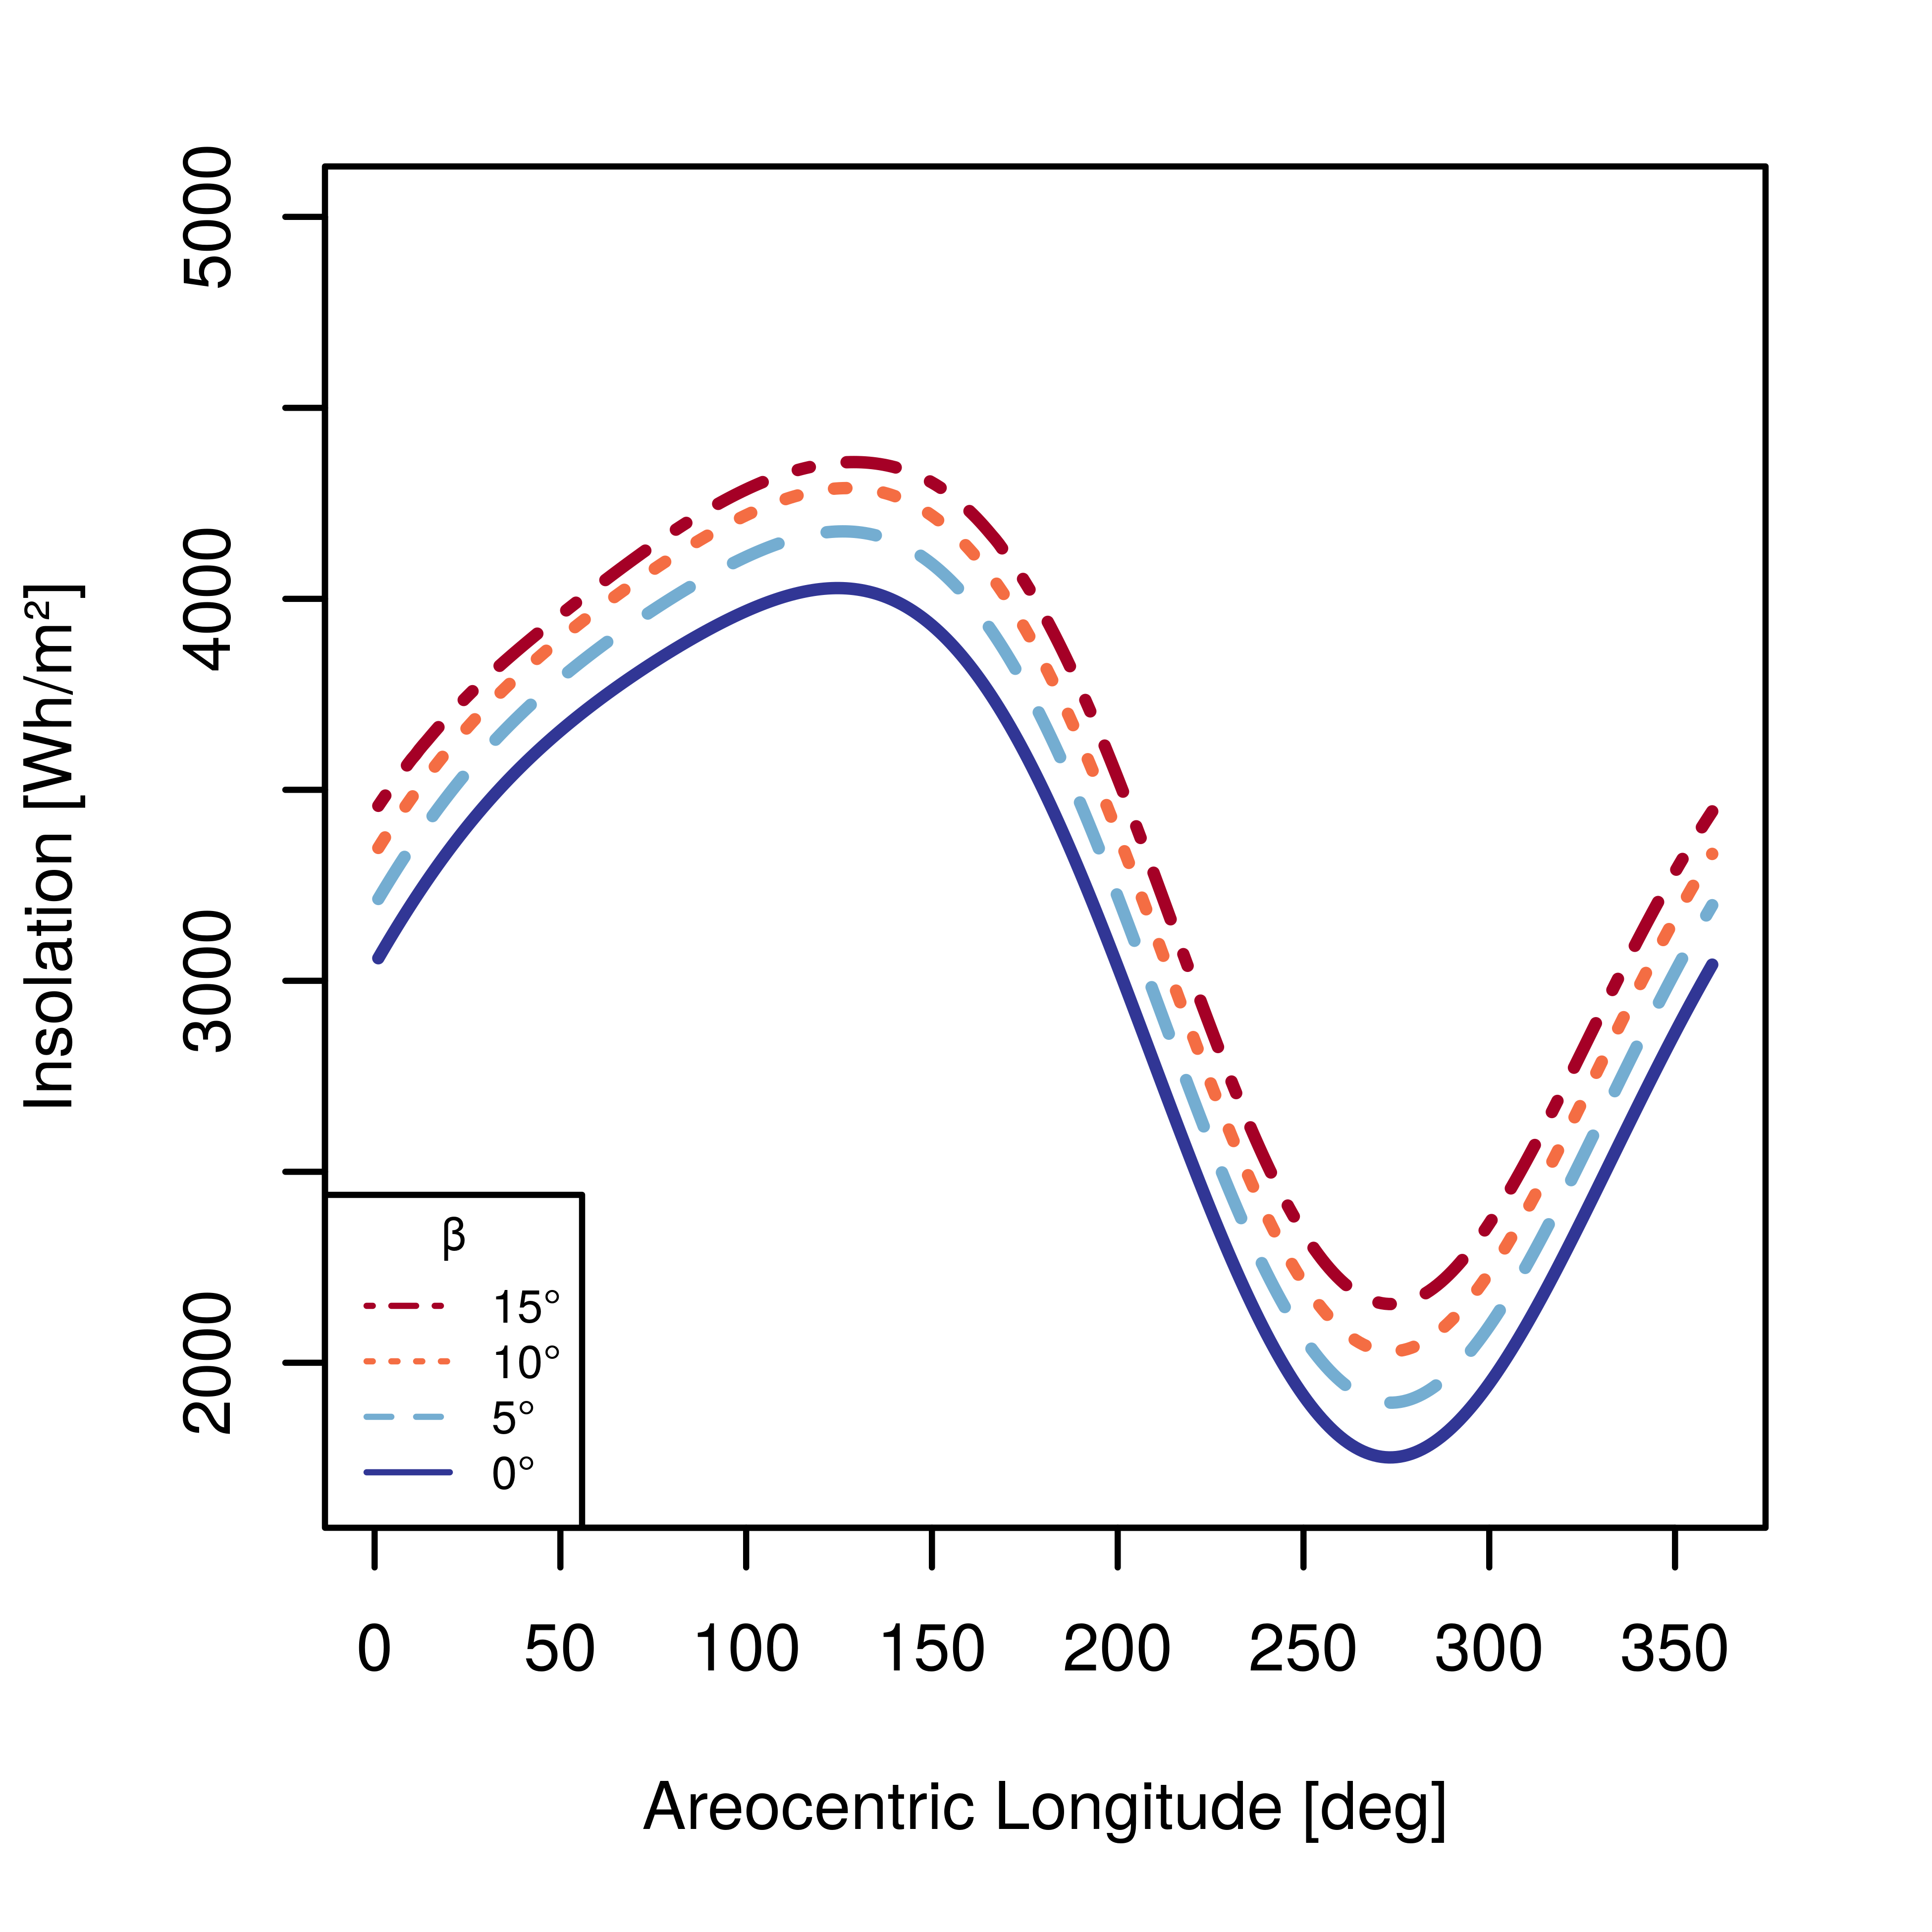
\includegraphics[height=\graphicsHeight]{sections/mars-solar-energy/mission-sites/plots/ismenius-cavus-solar-insolations-for-different-beta-inclinations.png}
            \subcaption{Ismenius Cavus.}
            \label{fig:plot:sub:solar-insolations-for-different-beta-ismenius-cavus}
    \end{subfigure}\\[0.8ex]
    \caption[Daily insolation at mission sites for different combinations of surface inclination and orientation angles]
    {Daily insolation at mission sites for different combinations of surface inclination and orientation angles.}
    \label{fig:plot:solar-insolations-for-different-beta}
\vspace{-2ex}
\end{figure}

Large values of $\beta$ are preferred at Ismenius Cavus, up to \SI{58}{\degree} for $\SI{255}{\degree} \leq L_{s} \leq \SI{285}{\degree}$. However, constraints imposed on the rover's active suspension system prevent it from attaining these inclinations. As such, the optimal $\beta$ angle from which maximum insolation can be achieved, henceforth referred to as $\beta_{opt}$, may not be attainable. In such cases, the best possible $\beta$ angle is targetted, hereinafter referred to as $\beta_{best}$. Body pitch commands of up to \SI{10}{\degree} are experimentally evaluated during steep slope climbing in \citeother{Cordes2018}. Modeling higher pitch angles resulted in poor wheel-ground contact angle, as shown in \refFig{fig:postures-sa-beta}. This is due to the wheel-steering axis having the same tilt as the rover's body. The rover's attainable tilt is thus restricted to a maximum of \SI{10}{\degree}.


\begin{figure}[h]
\captionsetup[subfigure]{justification=centering}
%\vspace{-2ex}
	\centering
    %% setup sizes
    \setlength{\subfigureWidth}{0.50\textwidth}
    \setlength{\graphicsHeight}{50mm}
    %% kill hyper-link highlighting
    \hypersetup{hidelinks=true}%
    %% the figures
    \begin{subfigure}[t]{\subfigureWidth}
        \centering
        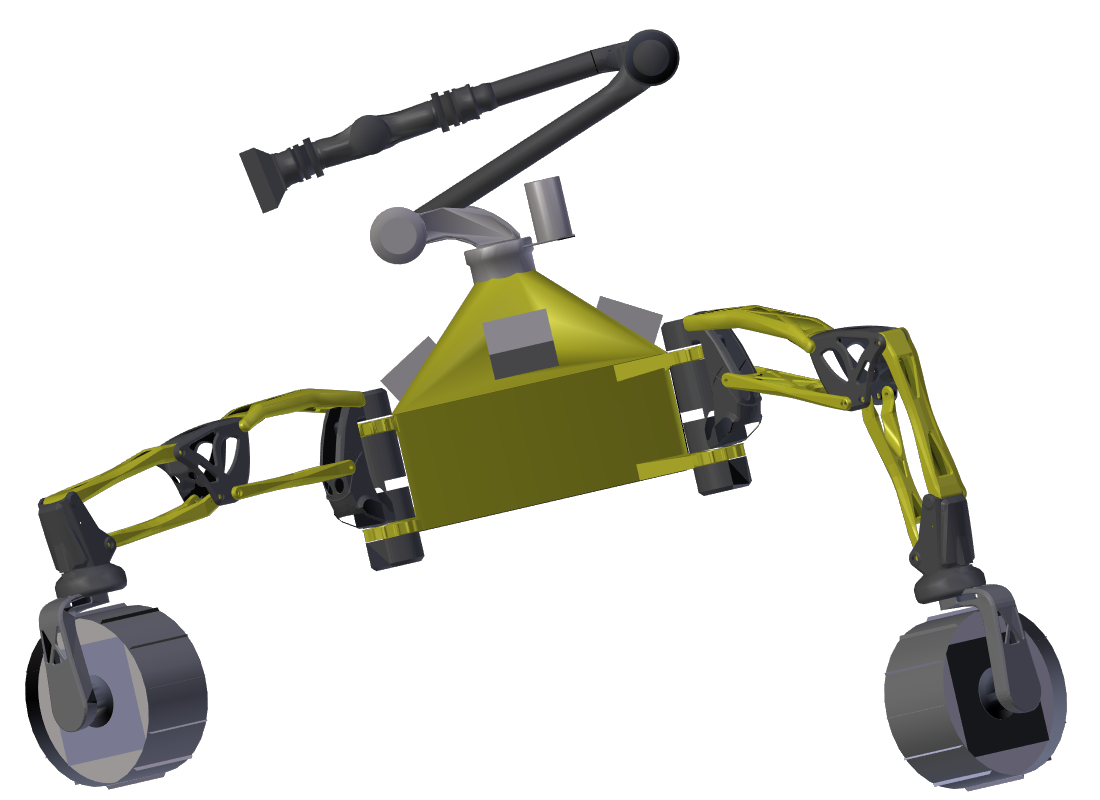
\includegraphics[height=\graphicsHeight]{sections/mars-solar-energy/mission-sites/images/sherpatt-render-surface-beta-13-deg.png}
        \subcaption{$\beta = \SI{13}{\degree}$}
        \label{fig:sub:postures-sa-beta-13-degree}
    \end{subfigure}\hfill
    \begin{subfigure}[t]{\subfigureWidth}
        \centering
        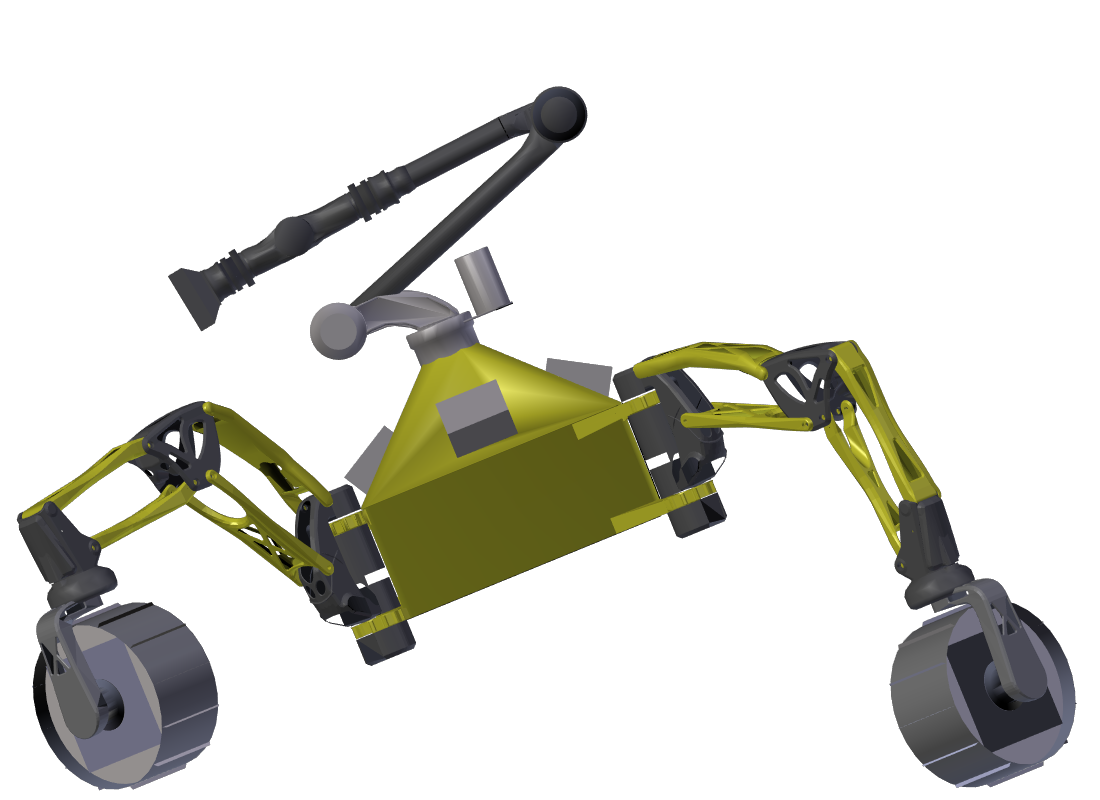
\includegraphics[height=\graphicsHeight]{sections/mars-solar-energy/mission-sites/images/sherpatt-render-surface-beta-22-deg.png}
  		\subcaption{$\beta = \SI{22}{\degree}$}
		\label{fig:sub:postures-sa-beta-22-degree}
	\end{subfigure}\\[0.8ex]
    \caption[SherpaTT body pitch \SI{13}{\degree} and \SI{22}{\degree}]
            {SherpaTT body pitch \SI{13}{\degree} and \SI{22}{\degree}.}
    \label{fig:postures-sa-beta}
\vspace{-2ex}
\end{figure}

\clearpage

Daily insolations on horizontal and inclined surfaces with $\beta_{best}=\pm\SI{10}{\degree}$\footnote{$\beta$ is positive in the northern hemisphere and negative in the southern hemisphere} are presented in Tables \ref{tab:insolation-iani-chaos-clear-and-dusty-days} and \ref{tab:insolation-iani-chaos-global-storm-days} for Iani Chaos and Tables \ref{tab:insolation-ismenius-cavus-clear-and-dusty-days} and \ref{tab:insolation-ismenius-cavus-global-storm-days} for Ismenius Cavus. Gains obtained in daily insolation with an inclined surface are more pronounced for sites further away from the equator. For a typical optical depth of $\tau = 0.4$, the average daily insolation gain on the inclined surface is approximately 7\% at Iani Chaos and 9\% at Ismenius Cavus.

\begin{table}[h]
\footnotesize
\centering
\caption[Worst- and best-case daily insolations for clear to dusty days at Iani Chaos]
{Worst- and best-case daily insolations for clear to dusty days at Iani Chaos. Daily insolation on an inclined surface $H_{\beta}$ was obtained with $\beta = \beta_{best} = \SI{-10}{\degree}$ and $\gamma_{c}$ set to optimal orientation angle.}
\label{tab:insolation-iani-chaos-clear-and-dusty-days}
\begin{tabular}{c|c|c|c|c|c|c|c|c|}
\cline{2-9}
\multicolumn{1}{l|}{} & \multicolumn{4}{c|}{\textbf{Worst Case}} & \multicolumn{4}{c|}{\textbf{Best Case}} \\ \hline
\multicolumn{1}{|c|}{$\tau$} & $L_{s}$ & $H_{h}$ & $H_{\beta}$ & $\%\:gain$ & $L_{s}$ & $H_{h}$ & $H_{\beta}$ & $\%\:gain$ \\ \hline
\multicolumn{1}{|c|}{\textbf{0.1}} & 80 & 3232 & 3721 & 15.13 & 221 & 5076 & 5695 & 12.19 \\ \hline
\multicolumn{1}{|c|}{\textbf{0.4}} & 81 & 2909 & 3166 & 8.85 & 218 & 4613 & 4933 & 6.93 \\ \hline
\multicolumn{1}{|c|}{\textbf{0.5}} & 81 & 2812 & 3025 & 7.58 & 218 & 4473 & 4736 & 5.89 \\ \hline
\multicolumn{1}{|c|}{\textbf{1.0}} & 82 & 2391 & 2479 & 3.67 & 214 & 3855 & 3959 & 2.69 \\ \hline
\multicolumn{1}{|c|}{\textbf{1.5}} & 82 & 2087 & 2125 & 1.81 & 213 & 3403 & 3444 & 1.19 \\ \hline
\end{tabular}
\end{table}


\begin{table}[h]
\footnotesize
\centering
\caption[Worst- and best-case daily insolations for global storm days at Iani Chaos]
{Worst- and best-case daily insolations for clear to global storm days at Iani Chaos. Daily insolation on an inclined surface $H_{\beta}$ was obtained with $\beta = \beta_{best} = \SI{-10}{\degree}$ and $\gamma_{c}$ set to optimal orientation angle.}
\label{tab:insolation-iani-chaos-global-storm-days}
\begin{tabular}{c|c|c|c|c|c|c|c|c|}
\cline{2-9}
\multicolumn{1}{l|}{} & \multicolumn{4}{c|}{\textbf{Worst Case}} & \multicolumn{4}{c|}{\textbf{Best Case}} \\ \hline
\multicolumn{1}{|c|}{$\tau$} & $L_{s}$ & $H_{h}$ & $H_{\beta}$ & $\%\:gain$ & $L_{s}$ & $H_{h}$ & $H_{\beta}$ & $\%\:gain$ \\ \hline
\multicolumn{1}{|c|}{\textbf{2.0}} & 360 & 2516 & 2519 & 0.10 & 212 & 3053 & 3066 & 0.42 \\ \hline
\multicolumn{1}{|c|}{\textbf{2.5}} & 360 & 2247 & 2243 & -0.18 & 211 & 2724 & 2723 & -0.02 \\ \hline
\multicolumn{1}{|c|}{\textbf{3.0}} & 360 & 1991 & 1985 & -0.32 & 210 & 2412 & 2406 & -0.27 \\ \hline
\multicolumn{1}{|c|}{\textbf{3.5}} & 360 & 1771 & 1763 & -0.45 & 210 & 2142 & 2134 & -0.37 \\ \hline
\multicolumn{1}{|c|}{\textbf{4.0}} & 360 & 1579 & 1572 & -0.44 & 209 & 1910 & 1901 & -0.47 \\ \hline
\multicolumn{1}{|c|}{\textbf{4.5}} & 360 & 1414 & 1406 & -0.54 & 209 & 1709 & 1700 & -0.54 \\ \hline
\multicolumn{1}{|c|}{\textbf{5.0}} & 360 & 1268 & 1261 & -0.58 & 209 & 1533 & 1523 & -0.62 \\ \hline
\end{tabular}
\end{table}


Due to the mostly diffuse composition of solar irradiance at higher optical depths, inclined surfaces become irrelevent during global dust storms. For $\tau \geq 2$, gains in daily insolation become negligeable at both mission sites.

\begin{table}[h]
\footnotesize
\centering
\caption[Worst- and best-case daily insolations for clear to dusty days at Ismenius Cavus]
{Worst- and best-case daily insolations for clear to dusty days at Ismenius Cavus. Daily insolation on an inclined surface $H_{\beta}$ was obtained with $\beta = \beta_{best} = \SI{10}{\degree}$ and $\gamma_{c}$ set to optimal orientation angle.}
\label{tab:insolation-ismenius-cavus-clear-and-dusty-days}
\begin{tabular}{c|c|c|c|c|c|c|c|c|}
\cline{2-9}
\multicolumn{1}{l|}{} & \multicolumn{4}{c|}{\textbf{Worst Case}} & \multicolumn{4}{c|}{\textbf{Best Case}} \\ \hline
\multicolumn{1}{|c|}{$\tau$} & $L_{s}$ & $H_{h}$ & $H_{\beta}$ & $\%\:gain$ & $L_{s}$ & $H_{h}$ & $H_{\beta}$ & $\%\:gain$ \\ \hline
\multicolumn{1}{|c|}{\textbf{0.1}} & 274 & 2102 & 2762 & 31.42 & 127 & 4421 & 4925 & 11.40 \\ \hline
\multicolumn{1}{|c|}{\textbf{0.4}} & 273 & 1752 & 2030 & 15.85 & 125 & 4028 & 4289 & 6.49 \\ \hline
\multicolumn{1}{|c|}{\textbf{0.5}} & 273 & 1655 & 1869 & 12.93 & 124 & 3908 & 4122 & 5.48 \\ \hline
\multicolumn{1}{|c|}{\textbf{1.0}} & 273 & 1284 & 1345 & 4.75 & 121 & 3378 & 3461 & 2.44 \\ \hline
\multicolumn{1}{|c|}{\textbf{1.5}} & 273 & 1045 & 1061 & 1.57 & 120 & 2945 & 2973 & 0.96 \\ \hline
\end{tabular}
\end{table}

\clearpage

\begin{table}[h]
\footnotesize
\centering
\caption[Worst- and best-case daily insolations for global storm days at Ismenius Cavus]
{Worst- and best-case daily insolations for clear to global storm days at Ismenius Cavus. Daily insolation on an inclined surface $H_{\beta}$ was obtained with $\beta = \beta_{best} = \SI{10}{\degree}$ and $\gamma_{c}$ set to optimal orientation angle.}
\label{tab:insolation-ismenius-cavus-global-storm-days}
\begin{tabular}{c|c|c|c|c|c|c|c|c|}
\cline{2-9}
\multicolumn{1}{l|}{} & \multicolumn{4}{c|}{\textbf{Worst Case}} & \multicolumn{4}{c|}{\textbf{Best Case}} \\ \hline
\multicolumn{1}{|c|}{$\tau$} & $L_{s}$ & $H_{h}$ & $H_{\beta}$ & $\%\:gain$ & $L_{s}$ & $H_{h}$ & $H_{\beta}$ & $\%\:gain$ \\ \hline
\multicolumn{1}{|c|}{\textbf{2.0}} & 273 & 901 & 904 & 0.30 & 180 & 2155 & 2155 & 0.00 \\ \hline
\multicolumn{1}{|c|}{\textbf{2.5}} & 273 & 783 & 782 & -0.17 & 180 & 1899 & 1891 & -0.43 \\ \hline
\multicolumn{1}{|c|}{\textbf{3.0}} & 273 & 677 & 675 & -028 & 180 & 1664 & 1654 & -0.61 \\ \hline
\multicolumn{1}{|c|}{\textbf{3.5}} & 273 & 589 & 586 & -0.48 & 180 & 1467 & 1456 & -0.75 \\ \hline
\multicolumn{1}{|c|}{\textbf{4.0}} & 273 & 516 & 514 & -0.35 & 180 & 1300 & 1290 & -0.80 \\ \hline
\multicolumn{1}{|c|}{\textbf{4.5}} & 273 & 462 & 460 & -0.37 & 180 & 1158 & 1149 & -0.80 \\ \hline
\multicolumn{1}{|c|}{\textbf{5.0}} & 273 & 424 & 422 & -0.54 & 180 & 1038 & 1028 & -0.98 \\ \hline
\end{tabular}
\end{table}



The worst-case slope traverse is an on inclined surface facing opposite the equator. This can be mitigated by using the rover's suspension system to compensate with a tilt in the opposite direction, as illustrated in \refFig{fig:sub:rover-on-slope-beta} where $B$ denotes the slope surface inclination angle and $\beta$ the \ac{SA} surface inclination angle.

\vspace{0.5cm}

\begin{figure}[h]
\captionsetup[subfigure]{justification=centering}
\vspace{-2ex}
	\centering
    %% setup sizes
    \setlength{\subfigureWidth}{0.50\textwidth}
    \setlength{\graphicsHeight}{40mm}
    %% kill hyper-link highlighting
    \hypersetup{hidelinks=true}%
    %% the figures
    \begin{subfigure}[t]{\subfigureWidth}
        \centering
        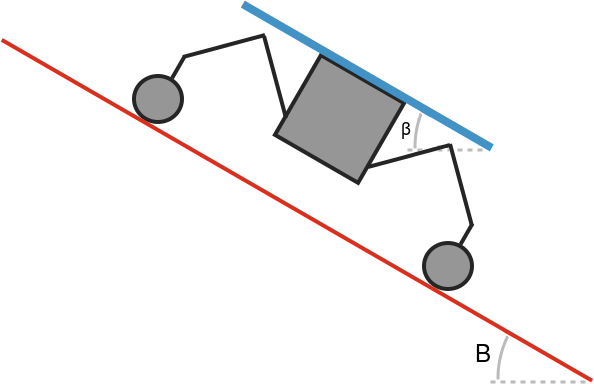
\includegraphics[height=\graphicsHeight]{sections/mars-solar-energy/mission-sites/images/stick-rover-beta-large.png}
        \subcaption{$\beta = B$}
        \label{fig:sub:rover-on-slope-beta-large}
    \end{subfigure}\hfill
    \begin{subfigure}[t]{\subfigureWidth}
        \centering
        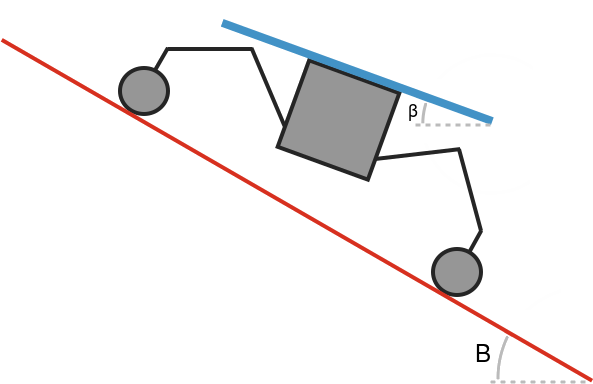
\includegraphics[height=\graphicsHeight]{sections/mars-solar-energy/mission-sites/images/stick-rover-beta-small.png}
  		\subcaption{$\beta < B$}
		\label{fig:sub:rover-on-slope-beta-small}
	\end{subfigure}\\[0.8ex]
    \caption[Rover on a slope using its active suspension system to reduce the \ac{SA} surface inclination angle]
            {Rover on a slope using its active suspension system to reduce the \ac{SA} surface inclination angle. Slope inclination angle $B = \SI{30}{\degree}$. In (a), $\beta = B = \SI{30}{\degree}$. In (b), the rover is tilted  \SI{10}{\degree} in the opposite direction of the slope so that $\beta = \SI{20}{\degree}$.}
    \label{fig:sub:rover-on-slope-beta}
\vspace{-2ex}
\end{figure}

By way of example, at Ismenius Cavus for $\tau = 0.4$ and $L_{s}=\SI{270}{\degree}$, descending a \SI{30}{\degree} slope bearing North results in a daily insolation of \SI{319}{Whm^{-2}}. This can be increased to \SI{767}{Whm^{-2}} by decreasing $\beta$ from \SI{30}{\degree} to \SI{25}{\degree} after tilting the rover southwards by \SI{5}{\degree} so that $\beta < B$ with $\beta = \SI{25}{\degree}$. A \SI{10}{\degree} tilt would increase the daily insolation to \SI{1046}{Whm^{-2}} with $\beta = \SI{20}{\degree}$.


\subsection{Summary}
Available solar insolation have been constrained by identifying two mission sites based on set of selection criteria. The need to navigate complex topographic morphologies at these sites also introduces considerations for \ac{SA} inclination strategies. Large differences in planetary latitudes between both sites ensures that several environmental variations are considered.


\section{Summary and Conclusion}
\label{sec:MarsSolarEnergy:SummaryAndConclusion}
Understanding the dynamics of the Martian solar radiation environment is a crucial prequisite to  conceptualizing feasible mission scenarios. In this chapter, the potenial solar power and energy outputs were constrainted with mission site selections. Two locations were identified so that rover task planning and \ac{SA} sizing processes may appreciate a richer set of consequences tied to a wider range of environmental variables.
